\section{NUMERICAL EXPERIMENTS}\label{sec:exp}

In order to motivate the need for a robust estimator of the gradient, we introduce three different examples of use of our estimator compared to existing approaches. All the code to reproduce the experiments and figures can be found at \url{https://git.sr.ht/~aussetg/locallinear}.

As our estimator is sensitive to the choice of hyperparameters $k$ and $\lambda$ we use a local leave-one-out procedure described in Algorithm~\ref{alg:localcv} for hyperparameter selection. As only the regression variable $Y$ is observed, the regression error is used as a proxy loss in the cross-validation. 
The high cost of $k$-NN is amortized by using $k$-d trees, bringing the total average complexity of the nearest neighbour search down to $O(n \log n)$. In cases where the aforementioned cost is too high ($n$ in the order of millions) it is possible to instead make use of approximate nearest neighbour schemes such as HNSW~\citep{malkovEfficientRobustApproximate2020}. Approximate Nearest Neighbours algorithms have recently enjoyed a regain of interest and provide high accuracy at a very low computational cost \citep{aumullerANNBenchmarksBenchmarkingTool2018}.
\begin{algorithm}
    \caption{Local Leave-One-Out}\label{alg:localcv}
    \begin{algorithmic}[1] %
        \Require $x$: sample point, $(X, Y)$: training set, $(K, \Lambda)$: grid
        \State{$X_{\text{LoO}} \gets \texttt{Neighbourhood of } x \texttt{ in } X \texttt{ of size } N$}
        \For{$k \in K, \lambda \in \Lambda$}
            \For{$X_i \in X_{\text{LoO}}$}
                \State{$m_i,  \beta_i \gets $ \texttt{estimated gradient at} $X_i$ \texttt{w.r.t} $X, Y$ \texttt{using}~\eqref{lll}}
            \EndFor
            \State{$\texttt{error}_{k, \lambda} \gets \frac{1}{N} \sum_{i=1}^N (m_i - Y_i)^2$}
        \EndFor
        \State{$k^\star, \lambda^\star \gets \argmin_{k, \lambda} \texttt{error}_{k, \lambda}$}
        \State{\textbf{return} $k^\star, \lambda^\star$}
    \end{algorithmic}
\end{algorithm}





\subsection{Variable Selection}

While a large number of observations is desirable the same is not necessarily the case for the individual features; a large number of features can be detrimental to the computational performance of most learning methods but also harmful to the predictive performance. In order to mitigate the detrimental impact of the high dimensionality, or \emph{curse of dimensionality}, one can try to reduce the effective dimension of the problem. A large body of work exists on dimensionality reduction as a preprocessing step that considers the intrinsic dimensionality of $X$ by considering for example that $X$ lies on a lower-dimensional manifold. Those approaches only consider $X$ in isolation and do not take into account $Y$ which is the variable of interest. It is possible to use the information in $Y$ to direct the dimension reduction of $X$, either by treating $Y$ as side information, as is done in~\cite{bachPredictiveLowrankDecomposition2005}, or by considering the existence of an explicit \emph{index space} such that $Y_i = g(v_1^\intercal X_i, \cdots, v_m^\intercal X_i) + \varepsilon_i$ as is done in~\cite{dalalyanNewAlgorithmEstimating2008}. In the latter case, it is possible to observe that the $\emph{index space}$ lies on the subspace spanned by the gradient.

In contrast with the work of~\cite{dalalyanNewAlgorithmEstimating2008} our approach is local and it is therefore possible to retrieve a different subspace in different regions of $\mathbb{R}^D$. As localizing the estimator increases its variance, we choose to only identify the dimensions of interest instead of estimating the full projection matrix.
We introduce \emph{Gradient Guided Trees} in Algorithm~\ref{alg:LocalLinearTree} to exploit the local aspect of our estimator in order to direct the cuts in a random tree: at each step, cuts are drawn randomly with probability proportional to estimated mean absolute gradient in the cell.
\begin{algorithm}
    \caption{Node Splitting for Gradient Guided Trees}\label{alg:LocalLinearTree}
    \begin{algorithmic}[1] %
        \Require $(X, Y)$: training set, $\texttt{Node}$: indexes of points in the node
        \State{$\nabla m (X_i) \gets \texttt{estimated gradient at } X_i, \, \forall i \in \texttt{Node}$ \texttt{ using }~\eqref{lll}}
        \State{$\omega \gets \sum_{i \in \texttt{Node}} \lvert \nabla m(X_i) \rvert$}
        \State{$K \gets$ \texttt{sample} $\sqrt{D}$ \texttt{dimensions in} $\{1, \ldots, d\} \texttt{ with probability weights} \propto \omega$}
        \State{$k, c \gets \texttt{best threshold } c \texttt{ and dimension } k$}
        \State{$\textbf{return } k, c$}
    \end{algorithmic}
\end{algorithm}
We demonstrate the improvements brought by guiding the cuts by the local information provided by the gradient by comparing the performance of a vanilla regression random forest with the same procedure but with local gradient information. 
We consider five datasets: the Breast Cancer Wisconsin (Diagnostic) Data Set introduced in~\cite{streetNuclearFeatureExtraction1993}; the Heart Disease dataset introduced by~\cite{detranoInternationalApplicationNew1989}; the classic Diamonds Price dataset; the Gasoline NIR dataset introduced by~\cite{kalivasTwoDataSets1997} and the Sloan Digital Sky Survey DR14 dataset of~\cite{abolfathiFourteenthDataRelease2018}. We measure the $L^2$ loss by cross validation across 50 folds using the same hyperparameters for the growing of the forest in both the standard and gradient guided variants.

We denote by RF, Random Forests grown from standard CART trees while GGF denote \emph{Gradient Guided Forests} grown from the \emph{Gradient Guided Trees} previously introduced. As seen in Table~\ref{table:results}, gradient guided split sampling consistently outperform the vanilla variant. When all variables are relevant, as is the case when the variables were carefully selected by the practitioner with prior knowledge, our variant performs similarly to the original algorithm while performance is greatly improved when only a few variables are relevant, such as in the NIR dataset~\citep{portierBootstrapTestingRank2014}.
\begin{table}
    \centering
    \begin{tabular}{@{}lrrrr@{}}
        & \multicolumn{2}{c}{Description} & \multicolumn{2}{c}{Loss} \\
        \cmidrule(l){2-3} \cmidrule(l){4-5}
        Dataset & $n$ & $D$ & RF & GGF \\
        \midrule
        Wisconsin & $569$ & $30$ & \thead{$0.0352$ \\ $\pm 3.29\cdot 10^{-4}$} & \thead{$\mathbf{0.0345}$ \\ $\pm 3.35 \cdot 10^{-4}$} \\
        Heart & $303$ & $13$ & \thead{$0.128$ \\ $\pm 6.6\cdot 10^{-4}$} & \thead{$\mathbf{0.124}$ \\ $\pm 8.6\cdot 10^{-4}$} \\
        Diamonds & $53940$ & $23$ & \thead{$680033$ \\ $\pm 3.45\cdot 10^{9}$} & \thead{$\mathbf{664265}$ \\ $\pm 2.81\cdot 10^{9}$} \\
        Gasoline & $60$ & $401$ & \thead{$0.678$ \\ $\pm 0.451$} & \thead{$\mathbf{0.512}$ \\ $\pm 0.347$} \\
        SDSS & $10000$ & $8$ & \thead{$0.872\cdot 10^{-3}$ \\ $\pm 4.50\cdot 10^{-6}$} & \thead{$\mathbf{0.776}\cdot 10^{-3}$ \\ $\pm 6.00\cdot 10^{-6}$} \\
        \bottomrule
    \end{tabular}
    \caption{Performance of the two random forest algorithms on a $50$-folds cross validation.}\label{table:results}
\end{table}


\subsection{Gradient Free Optimization}

Many of the recent advances in the field of machine learning have been made possible in one way or another by advances in optimization; both in how well we are able to optimize complex function and what type of functions we are able to optimize if only locally. Recent advances in automatic differentiation as well as advances that push the notion of \emph{what} can be differentiated have given rise to the notion of \emph{differentiable programming}~\citep{innesDifferentiableProgrammingSystem2019} in which a significant body of work can be expressed as the solution to a minimization problem usually then solved by gradient descent.

We study here the use of the local linear estimator of the gradient in Algorithm~\ref{alg:lolamin} in cases where analytic or automatic differentiation is impossible, and compare it to a standard gradient free optimization technique as well as the oracle where the true gradient is known.
\begin{algorithm}
    \caption{Estimated Gradient Descent}\label{alg:lolamin}
    \begin{algorithmic}[1] %
        \Require $x_0$: initial guess, $f$: function $\mathbb{R}^D \to \mathbb{R}$, $M$: budget
        \State{$X \gets X_1, \ldots, X_M \texttt{ with } X_i \sim \mathcal{N}(x_0, \varepsilon \times I_D)$}\label{alg:lolamin:line1}
        \State{$Y \gets f(X) := f(X_1), \ldots, f(X_M)$}
        \While{\texttt{not StoppingCondition}}
            \State{$m, \Delta \gets$ \texttt{estimated gradient at} $x$ \texttt{w.r.t} $X, Y$ \texttt{using}~\eqref{lll}}\label{alg:lolamin:line5}
            \State{$X \gets X, X_1, \ldots, X_M \texttt{ with } X_i \sim \mathcal{N}(\texttt{GradientStep}(x, \Delta), \varepsilon \times I_D)$}
            \State{$Y \gets f(X)$}
            \State{$x \gets \argmin_{X_i} \{ f(X_i) \}$}
        \EndWhile
        \State{$\textbf{return } x$}
    \end{algorithmic}
\end{algorithm}
While line~\texttt{1} bears resemblance with Gaussian smoothing and could therefore be seen as analogous to gradient estimation via Gaussian smoothing (see~\cite{berahasTheoreticalEmpiricalComparison2020}), two key differences here are the subsequent local linear step as well as the fact that the samples from line~\ref{alg:lolamin:line1} are not necessarily the samples used in the local linear estimator of line~\ref{alg:lolamin:line5}. 

We first minimize the standard but challenging Rosenbrock function for different values of $d$. which is defined as
\begin{align}
    f(x) = 100 \sum_{i=1}^{d-1} (x_{i+1} - x_i)^2 + (x_i - 1)^2.
\end{align}
We compare for reference our approach to the Nelder-Mead (simplex search) algorithm; a standard gradient free optimization technique.
It is apparent in Figure~\ref{fig:rosenbrock_grad} that estimating the gradient yields a significant advantage compared to traditional gradient-free techniques that usually have to rely on bounding arguments and feasible regions and therefore scale unfavourably with the dimension. As our approach uses a nearest neighbours formulation for the gradient estimate, we are able to efficiently reuse past samples in the current estimate of the gradient; this makes it possible to achieve a sufficiently accurate estimate of the gradient even in high dimensions.
\begin{figure}
    \centering
    \begin{subfigure}[t]{1.\linewidth}
        \centering
        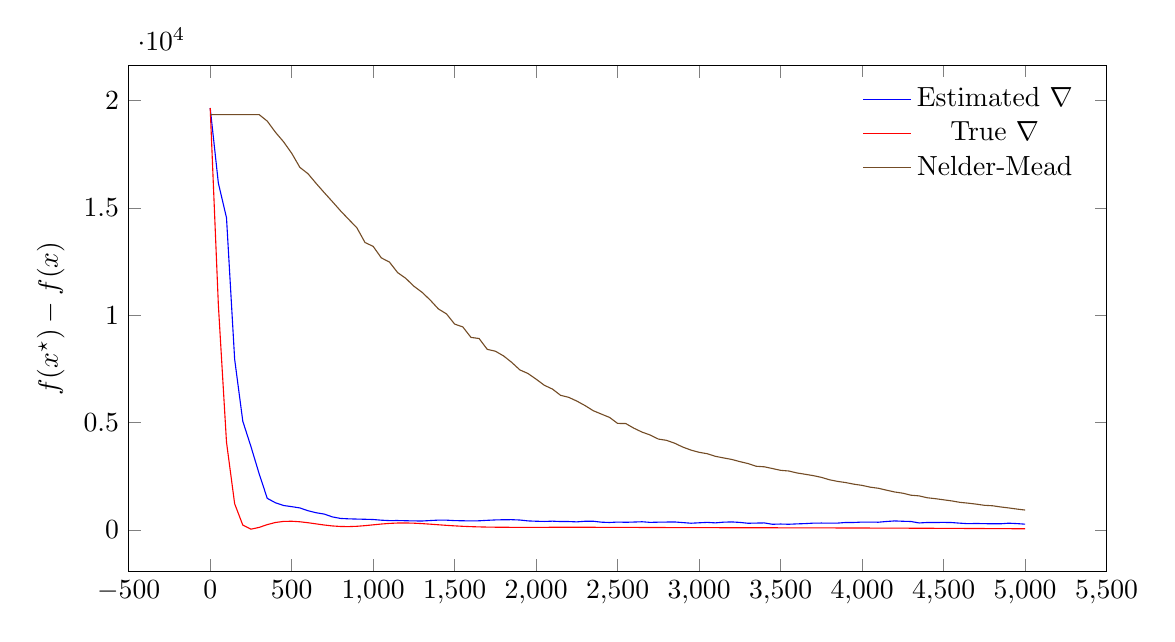
\begin{tikzpicture}
\begin{axis}[ylabel={$\lvert f(x^\star) - f(x) \rvert$},width=14cm,height=8cm, legend style={draw=none}]
    \legend{{Estimated $\nabla$},{True $\nabla$},{Nelder-Mead}}
    \addplot+[no marks]
        table[x expr=\thisrowno{0}*50, row sep={\\}]
        {
            x  y  \\
            0.0  19649.0  \\
            1.0  16155.658771712246  \\
            2.0  14540.33361942822  \\
            3.0  7953.599475253909  \\
            4.0  5066.529746982929  \\
            5.0  3886.832369333254  \\
            6.0  2628.899079375951  \\
            7.0  1476.3695468645078  \\
            8.0  1271.4826624754114  \\
            9.0  1142.4637792652413  \\
            10.0  1089.1514063738682  \\
            11.0  1029.087477354468  \\
            12.0  900.2864550286253  \\
            13.0  805.0196358739224  \\
            14.0  743.2740632819655  \\
            15.0  610.5976523302126  \\
            16.0  539.7884051582201  \\
            17.0  521.1446518188443  \\
            18.0  510.9304060098636  \\
            19.0  501.1102493655367  \\
            20.0  490.19709616804346  \\
            21.0  458.2924464721199  \\
            22.0  439.6581967766843  \\
            23.0  442.50391473894575  \\
            24.0  432.8480546732227  \\
            25.0  424.6223986048977  \\
            26.0  420.9313682512128  \\
            27.0  441.6954996175187  \\
            28.0  462.24434928054524  \\
            29.0  460.22485329545276  \\
            30.0  438.5720084119326  \\
            31.0  431.1659019451867  \\
            32.0  425.4331163044947  \\
            33.0  430.3903226554454  \\
            34.0  452.49903527256345  \\
            35.0  470.33389981133826  \\
            36.0  480.1486634870575  \\
            37.0  481.8751225180056  \\
            38.0  466.69944545930724  \\
            39.0  424.8640485577546  \\
            40.0  410.02294018317946  \\
            41.0  399.78520882446514  \\
            42.0  412.92699245751345  \\
            43.0  396.20535119001914  \\
            44.0  395.1831368505887  \\
            45.0  380.3582852998892  \\
            46.0  408.9420872504598  \\
            47.0  410.7032197417549  \\
            48.0  366.1916962871619  \\
            49.0  351.48724881936147  \\
            50.0  371.44711771616164  \\
            51.0  360.99420493534495  \\
            52.0  372.18058467917024  \\
            53.0  385.42088738787606  \\
            54.0  356.5772799534951  \\
            55.0  366.3206278545177  \\
            56.0  371.54982356370067  \\
            57.0  375.41289139997065  \\
            58.0  347.24851854542084  \\
            59.0  317.14026704500975  \\
            60.0  337.19830384338746  \\
            61.0  356.6666679649715  \\
            62.0  333.57107309416335  \\
            63.0  366.46567392524383  \\
            64.0  377.3081965464865  \\
            65.0  355.1363547384735  \\
            66.0  315.661719294923  \\
            67.0  324.10310825438415  \\
            68.0  331.23587975310716  \\
            69.0  268.30718354082836  \\
            70.0  279.687760239002  \\
            71.0  268.80244115323757  \\
            72.0  286.4403121249994  \\
            73.0  299.91528050175066  \\
            74.0  320.87521389724054  \\
            75.0  325.4828033934373  \\
            76.0  321.14081812579667  \\
            77.0  323.07530231321954  \\
            78.0  352.9582954256946  \\
            79.0  352.79290232904344  \\
            80.0  370.48510431829783  \\
            81.0  368.77787906679777  \\
            82.0  364.417268353134  \\
            83.0  398.512951860813  \\
            84.0  424.0853972129796  \\
            85.0  408.34372729469146  \\
            86.0  397.6457164887654  \\
            87.0  329.7523148962795  \\
            88.0  352.00633695454394  \\
            89.0  351.0124503482705  \\
            90.0  355.46601440822485  \\
            91.0  348.35704004031277  \\
            92.0  319.83211873186167  \\
            93.0  295.83821923970913  \\
            94.0  306.05790730967914  \\
            95.0  296.49284107838645  \\
            96.0  292.69607600059953  \\
            97.0  291.07434362540283  \\
            98.0  318.90518352925477  \\
            99.0  300.07235600872195  \\
            100.0  273.3408910376874  \\
        }
        ;
    \addplot+[no marks]
        table[x expr=\thisrowno{0}*50, row sep={\\}]
        {
            x  y  \\
            0.0  19649.0  \\
            1.0  10493.529109000005  \\
            2.0  4091.6665508738497  \\
            3.0  1224.840320714823  \\
            4.0  230.35761544396163  \\
            5.0  39.797239868808774  \\
            6.0  122.28441400010296  \\
            7.0  252.382789258519  \\
            8.0  351.1214178922489  \\
            9.0  401.6198109115192  \\
            10.0  409.2916677760125  \\
            11.0  385.1996320795456  \\
            12.0  340.69578733525645  \\
            13.0  286.6623874280347  \\
            14.0  233.53670937304244  \\
            15.0  190.63523579926024  \\
            16.0  164.90940508596114  \\
            17.0  159.77007953734147  \\
            18.0  174.4830215136091  \\
            19.0  204.4185052489429  \\
            20.0  242.2093168389787  \\
            21.0  279.56395511048805  \\
            22.0  309.20483860438645  \\
            23.0  326.34138215832735  \\
            24.0  329.2932573332362  \\
            25.0  319.22411110663296  \\
            26.0  299.24930783155406  \\
            27.0  273.32155832907534  \\
            28.0  245.25674255713466  \\
            29.0  218.10527673209404  \\
            30.0  193.90048122370433  \\
            31.0  173.69747094429115  \\
            32.0  157.77480622789983  \\
            33.0  145.88671545892194  \\
            34.0  137.49366403281388  \\
            35.0  131.93853830227974  \\
            36.0  128.56329692036945  \\
            37.0  126.77530166815778  \\
            38.0  126.07710885191057  \\
            39.0  126.07259915236149  \\
            40.0  126.45934917235309  \\
            41.0  127.01413616662428  \\
            42.0  127.576246803737  \\
            43.0  128.03181847630674  \\
            44.0  128.3013564937708  \\
            45.0  128.33144452441377  \\
            46.0  128.09042676280103  \\
            47.0  127.56677214210852  \\
            48.0  126.7683234794665  \\
            49.0  125.72085527349043  \\
            50.0  124.46511564605815  \\
            51.0  123.05238868876414  \\
            52.0  121.53921169495142  \\
            53.0  119.98207802425144  \\
            54.0  118.43283281040348  \\
            55.0  116.93519909571403  \\
            56.0  115.5226003769336  \\
            57.0  114.21724076559435  \\
            58.0  113.03027556191829  \\
            59.0  111.96283741171847  \\
            60.0  111.00765852987176  \\
            61.0  110.15103482211356  \\
            62.0  109.37490398223572  \\
            63.0  108.65884916539491  \\
            64.0  107.98188583163714  \\
            65.0  107.32393622066748  \\
            66.0  106.6669396999306  \\
            67.0  105.9955855371754  \\
            68.0  105.29768623171422  \\
            69.0  104.56423378737392  \\
            70.0  103.78919797081741  \\
            71.0  102.969134718051  \\
            72.0  102.10267486185774  \\
            73.0  101.18995915761688  \\
            74.0  100.23207654777568  \\
            75.0  99.2305504116358  \\
            76.0  98.1869039802857  \\
            77.0  97.1023227939026  \\
            78.0  95.97742033564084  \\
            79.0  94.8121036371564  \\
            80.0  93.60552909451764  \\
            81.0  92.35613493605919  \\
            82.0  91.06173542613445  \\
            83.0  89.7196624743463  \\
            84.0  88.32694228127224  \\
            85.0  86.88049742911869  \\
            86.0  85.37736791429356  \\
            87.0  83.81494758797957  \\
            88.0  82.19123496188377  \\
            89.0  80.50509904736639  \\
            90.0  78.75656156047695  \\
            91.0  76.94709619299199  \\
            92.0  75.07994347814841  \\
            93.0  73.16043584498586  \\
            94.0  71.19632158876317  \\
            95.0  69.19806865121758  \\
            96.0  67.17911952296514  \\
            97.0  65.15605789359572  \\
            98.0  63.148637145578604  \\
            99.0  61.1796124807609  \\
            100.0  59.27431533436742  \\
        }
        ;
    \addplot+[no marks]
        table[x expr=\thisrowno{0}*50, row sep={\\}]
        {
            x  y  \\
            0.0  19344.0625  \\
            1.0  19344.0625  \\
            2.0  19344.0625  \\
            3.0  19344.0625  \\
            4.0  19344.0625  \\
            5.0  19344.0625  \\
            6.0  19344.0625  \\
            7.0  19040.092169750224  \\
            8.0  18524.091708941967  \\
            9.0  18078.959202617356  \\
            10.0  17543.944194147174  \\
            11.0  16887.11488119078  \\
            12.0  16590.60733325794  \\
            13.0  16139.122656892067  \\
            14.0  15708.334064245542  \\
            15.0  15288.847912542666  \\
            16.0  14860.846246339614  \\
            17.0  14462.695679980867  \\
            18.0  14072.253144954955  \\
            19.0  13386.867320536729  \\
            20.0  13207.53413317501  \\
            21.0  12671.927104325581  \\
            22.0  12475.315176135135  \\
            23.0  11986.903806366483  \\
            24.0  11718.904847602129  \\
            25.0  11350.54901995632  \\
            26.0  11069.444203814453  \\
            27.0  10707.169594976122  \\
            28.0  10296.14689351034  \\
            29.0  10062.253730920318  \\
            30.0  9588.116654897349  \\
            31.0  9457.421628852115  \\
            32.0  8970.06648716477  \\
            33.0  8917.132009239825  \\
            34.0  8413.277094104265  \\
            35.0  8325.935799795505  \\
            36.0  8107.873065786172  \\
            37.0  7806.80161702764  \\
            38.0  7456.260058782211  \\
            39.0  7287.837387013737  \\
            40.0  7023.855486295726  \\
            41.0  6741.016467171516  \\
            42.0  6564.391148949375  \\
            43.0  6271.939122771003  \\
            44.0  6178.354215054734  \\
            45.0  6002.6668961953055  \\
            46.0  5795.529060359419  \\
            47.0  5558.010757585843  \\
            48.0  5399.286008722213  \\
            49.0  5245.9617521582695  \\
            50.0  4964.550601753458  \\
            51.0  4957.7878812103245  \\
            52.0  4740.294914811976  \\
            53.0  4559.7656167567375  \\
            54.0  4424.252165802021  \\
            55.0  4235.6598161059155  \\
            56.0  4176.6665265345655  \\
            57.0  4042.2010298601404  \\
            58.0  3862.351531324698  \\
            59.0  3722.092209739732  \\
            60.0  3619.1703401193545  \\
            61.0  3552.9628431905758  \\
            62.0  3432.2131896959577  \\
            63.0  3357.666870024197  \\
            64.0  3287.1557287106048  \\
            65.0  3185.3559133609997  \\
            66.0  3095.9856534410187  \\
            67.0  2969.2494004411838  \\
            68.0  2944.446995088319  \\
            69.0  2862.8158128247533  \\
            70.0  2780.3733413878763  \\
            71.0  2748.8560851179195  \\
            72.0  2658.234385640356  \\
            73.0  2597.932529081191  \\
            74.0  2534.2518493186667  \\
            75.0  2452.9690847414413  \\
            76.0  2340.055889560737  \\
            77.0  2263.9611283700574  \\
            78.0  2209.4093175757066  \\
            79.0  2134.627381133115  \\
            80.0  2079.3337642311258  \\
            81.0  1995.953904389224  \\
            82.0  1944.96504627987  \\
            83.0  1855.780752602561  \\
            84.0  1771.9221667062923  \\
            85.0  1715.08886370242  \\
            86.0  1621.829173686692  \\
            87.0  1589.6145845677313  \\
            88.0  1501.9676131795588  \\
            89.0  1459.9152747248122  \\
            90.0  1407.8215411811807  \\
            91.0  1355.9570795399636  \\
            92.0  1289.7551842515654  \\
            93.0  1251.985377254327  \\
            94.0  1207.1439508305446  \\
            95.0  1151.3550990090562  \\
            96.0  1130.7773506668277  \\
            97.0  1075.2707627327952  \\
            98.0  1029.2416644133352  \\
            99.0  976.4373149901232  \\
            100.0  931.2869866818664  \\
        }
        ;
\end{axis}
\end{tikzpicture}
 %
    \end{subfigure}
    \hfill
    \begin{subfigure}[t]{1.\linewidth}
        \centering
        \begin{tikzpicture}
\begin{axis}[xlabel={\# function evaluations},width=24cm,height=15cm, ylabel={$\lvert f(x^\star) - f(x) \rvert$}, xtick={0,2500,5000}, legend style={draw=none}]
\legend{{Ours},{True $\nabla$},{Nelder-Mead}}
    \addplot+[no marks]
        table[x expr=\thisrowno{0}*50, row sep={\\}]
        {
            x  y  \\
            0.0  39699.0  \\
            1.0  38661.01222013547  \\
            2.0  38257.07661628965  \\
            3.0  37307.40555030072  \\
            4.0  36602.470842273106  \\
            5.0  35187.67089026399  \\
            6.0  32339.80554213424  \\
            7.0  31625.676311979743  \\
            8.0  27096.45117682102  \\
            9.0  22356.300295364614  \\
            10.0  21056.046623936476  \\
            11.0  20076.539398271583  \\
            12.0  17850.2852131037  \\
            13.0  17066.183387951365  \\
            14.0  17165.875858373205  \\
            15.0  16974.783045671284  \\
            16.0  16644.828990279144  \\
            17.0  17180.256171648292  \\
            18.0  16525.489917713432  \\
            19.0  15854.614862582781  \\
            20.0  10939.669669772113  \\
            21.0  7639.746669158685  \\
            22.0  6707.588190227669  \\
            23.0  6155.088924048022  \\
            24.0  6382.423708635092  \\
            25.0  5356.973320599942  \\
            26.0  5194.4206390614445  \\
            27.0  4242.043502428031  \\
            28.0  3909.536331868685  \\
            29.0  3740.7256196643966  \\
            30.0  3013.393872006049  \\
            31.0  2654.119323199185  \\
            32.0  2459.8880243732046  \\
            33.0  2065.985878970206  \\
            34.0  2154.1258265404485  \\
            35.0  2192.4021877373616  \\
            36.0  2203.628613898691  \\
            37.0  2122.413339031094  \\
            38.0  2309.38291617143  \\
            39.0  2253.4912448406862  \\
            40.0  2226.398050930897  \\
            41.0  2056.991592699621  \\
            42.0  2103.1192672383145  \\
            43.0  2050.5688941048893  \\
            44.0  1780.9849366516366  \\
            45.0  1505.9943010545148  \\
            46.0  1572.7017037559315  \\
            47.0  1658.569660939209  \\
            48.0  1758.740702274854  \\
            49.0  1491.2098560520756  \\
            50.0  1524.3858614778053  \\
            51.0  1535.5870766859675  \\
            52.0  1431.90564578395  \\
            53.0  1472.6553228053672  \\
            54.0  1493.6111687436096  \\
            55.0  1449.9719738499484  \\
            56.0  1470.6942397904957  \\
            57.0  1568.550997603763  \\
            58.0  1574.3229264539311  \\
            59.0  1602.4832036660457  \\
            60.0  1567.5408877480359  \\
            61.0  1653.5290649494857  \\
            62.0  1650.9313659397853  \\
            63.0  1693.5480324658538  \\
            64.0  1676.1196539855512  \\
            65.0  1564.6304202404772  \\
            66.0  1616.9532580748146  \\
            67.0  1651.7083854074444  \\
            68.0  1678.0067702696274  \\
            69.0  1650.4952403645864  \\
            70.0  1599.6737806855306  \\
            71.0  1563.111361569664  \\
            72.0  1602.452680047029  \\
            73.0  1598.0720288866387  \\
            74.0  1599.4361730825474  \\
            75.0  1607.5861611398384  \\
            76.0  1561.561154541469  \\
            77.0  1628.2205949300949  \\
            78.0  1662.4810842207805  \\
            79.0  1631.8231558327486  \\
            80.0  1654.2652710232778  \\
            81.0  1571.6474432727462  \\
            82.0  1562.4142535001747  \\
            83.0  1647.6329477249467  \\
            84.0  1569.7630453063884  \\
            85.0  1586.7571033939148  \\
            86.0  1533.0532205245609  \\
            87.0  1480.4316203841272  \\
            88.0  1377.8650908815393  \\
            89.0  1293.9893767798308  \\
            90.0  1248.4522276279633  \\
            91.0  1207.9070289455703  \\
            92.0  1200.5171803247856  \\
            93.0  1237.2485502685831  \\
            94.0  1296.622428896029  \\
            95.0  1345.4256942212473  \\
            96.0  1236.562856916525  \\
            97.0  1270.5819635850073  \\
            98.0  1268.3832101487653  \\
            99.0  1166.532804745176  \\
            100.0  1219.851441261067  \\
        }
        ;
    \addplot+[no marks]
        table[x expr=\thisrowno{0}*50, row sep={\\}]
        {
            x  y  \\
            0.0  39699.0  \\
            1.0  21273.580159  \\
            2.0  8361.816535773676  \\
            3.0  2528.453552575729  \\
            4.0  467.2838146610457  \\
            5.0  41.64359192538598  \\
            6.0  182.63178866081125  \\
            7.0  431.5842617044014  \\
            8.0  623.8317479395903  \\
            9.0  720.7492707978596  \\
            10.0  730.7930660476478  \\
            11.0  676.1329444211493  \\
            12.0  580.8430716739987  \\
            13.0  467.9497161883569  \\
            14.0  358.72193086904474  \\
            15.0  271.5017376129448  \\
            16.0  219.78799158105423  \\
            17.0  210.25544525591744  \\
            18.0  241.53860734598283  \\
            19.0  304.48711957723856  \\
            20.0  384.22671793795405  \\
            21.0  463.6946297553302  \\
            22.0  527.6400576173379  \\
            23.0  565.8192022869789  \\
            24.0  574.4587969030347  \\
            25.0  555.8033772717197  \\
            26.0  516.2747493060102  \\
            27.0  464.1212827767793  \\
            28.0  407.3514024125243  \\
            29.0  352.3959747387081  \\
            30.0  303.56510674815604  \\
            31.0  263.11574604503437  \\
            32.0  231.66302028502355  \\
            33.0  208.7023361756356  \\
            34.0  193.09184220873672  \\
            35.0  183.42565955920026  \\
            36.0  178.28489605846715  \\
            37.0  176.38354712772963  \\
            38.0  176.63678031676616  \\
            39.0  178.1782288824284  \\
            40.0  180.34738729193037  \\
            41.0  182.66200487449672  \\
            42.0  184.78530743975975  \\
            43.0  186.4942635344483  \\
            44.0  187.65253860863677  \\
            45.0  188.18972317000706  \\
            46.0  188.0866542481925  \\
            47.0  187.36532165560433  \\
            48.0  186.0812489136271  \\
            49.0  184.31645948965308  \\
            50.0  182.17193825463377  \\
            51.0  179.7594248459017  \\
            52.0  177.19304090498895  \\
            53.0  174.58150738719397  \\
            54.0  172.02162787171306  \\
            55.0  169.59347018999946  \\
            56.0  167.35741556303523  \\
            57.0  165.35303220732416  \\
            58.0  163.5995819050226  \\
            59.0  162.0978724073498  \\
            60.0  160.8331134474459  \\
            61.0  159.77841233260745  \\
            62.0  158.89855241241023  \\
            63.0  158.15373009403868  \\
            64.0  157.50297822756346  \\
            65.0  156.90706935873055  \\
            66.0  156.33076494295375  \\
            67.0  155.74434968457808  \\
            68.0  155.1244577715795  \\
            69.0  154.45425484470303  \\
            70.0  153.72308228575966  \\
            71.0  152.92569673336857  \\
            72.0  152.06124744803984  \\
            73.0  151.1321289089565  \\
            74.0  150.14282895920016  \\
            75.0  149.09886792394397  \\
            76.0  148.00589560222272  \\
            77.0  146.86898466050644  \\
            78.0  145.69213367816235  \\
            79.0  144.47797280836568  \\
            80.0  143.2276505803083  \\
            81.0  141.94087175663506  \\
            82.0  140.6160527142863  \\
            83.0  139.25056150205538  \\
            84.0  137.84101336328845  \\
            85.0  136.38359794331987  \\
            86.0  134.87442060947228  \\
            87.0  133.30984646229734  \\
            88.0  131.68684106484008  \\
            89.0  130.00330618105275  \\
            90.0  128.25841153924927  \\
            91.0  126.45292455084338  \\
            92.0  124.58953880311108  \\
            93.0  122.67319883916852  \\
            94.0  120.71141314184341  \\
            95.0  118.71453939109142  \\
            96.0  116.69601626020405  \\
            97.0  114.67250496374535  \\
            98.0  112.66389279060171  \\
            99.0  110.69310206179976  \\
            100.0  108.78564433474222  \\
        }
        ;
    \addplot+[no marks]
        table[x expr=\thisrowno{0}*50, row sep={\\}]
        {
            x  y  \\
            0.0  39394.0625  \\
            1.0  39394.0625  \\
            2.0  39394.0625  \\
            3.0  39394.0625  \\
            4.0  39394.0625  \\
            5.0  39394.0625  \\
            6.0  39394.0625  \\
            7.0  39394.0625  \\
            8.0  39394.0625  \\
            9.0  39394.0625  \\
            10.0  39394.0625  \\
            11.0  39394.0625  \\
            12.0  39394.0625  \\
            13.0  39394.0625  \\
            14.0  39394.0625  \\
            15.0  39394.0625  \\
            16.0  39394.0625  \\
            17.0  39274.30789875409  \\
            18.0  38861.297505809955  \\
            19.0  38736.19398394994  \\
            20.0  38558.40206737832  \\
            21.0  38142.85151860562  \\
            22.0  38053.9821995296  \\
            23.0  37900.041725084164  \\
            24.0  37498.23671284519  \\
            25.0  37414.318012602715  \\
            26.0  37284.37348967827  \\
            27.0  37135.97542465081  \\
            28.0  36885.121878349084  \\
            29.0  36716.14068281262  \\
            30.0  36566.67958463693  \\
            31.0  36300.95570826876  \\
            32.0  36204.77416164554  \\
            33.0  36012.49285673085  \\
            34.0  35690.630481721084  \\
            35.0  35677.31366360184  \\
            36.0  35503.53892295225  \\
            37.0  35339.05752031292  \\
            38.0  35083.42021978587  \\
            39.0  34924.57304411732  \\
            40.0  34819.45090356014  \\
            41.0  34511.27630089908  \\
            42.0  34423.04277448081  \\
            43.0  34325.76740911861  \\
            44.0  34177.5952944901  \\
            45.0  33933.522708610464  \\
            46.0  33830.12241985861  \\
            47.0  33694.56254240225  \\
            48.0  33359.70426564397  \\
            49.0  33332.16734520328  \\
            50.0  33198.137994731915  \\
            51.0  33048.604272654906  \\
            52.0  32831.012467805784  \\
            53.0  32648.49374090282  \\
            54.0  32549.607212853974  \\
            55.0  32270.116232076034  \\
            56.0  32223.596597502776  \\
            57.0  32076.06493505476  \\
            58.0  31738.873773904113  \\
            59.0  31725.255026324594  \\
            60.0  31614.92836996697  \\
            61.0  31414.417433247505  \\
            62.0  31263.98627715653  \\
            63.0  31107.591173260756  \\
            64.0  30980.153591604118  \\
            65.0  30765.69058462394  \\
            66.0  30670.9267500321  \\
            67.0  30540.24764192069  \\
            68.0  30259.822436661492  \\
            69.0  30234.333006608093  \\
            70.0  30066.236929886585  \\
            71.0  29743.718471152937  \\
            72.0  29743.247840416567  \\
            73.0  29607.54133264848  \\
            74.0  29468.396012573707  \\
            75.0  29274.329501902645  \\
            76.0  29160.682339442148  \\
            77.0  29023.109378307825  \\
            78.0  28768.578983576237  \\
            79.0  28720.607805105607  \\
            80.0  28583.488661506268  \\
            81.0  28288.34204402337  \\
            82.0  28248.402747576998  \\
            83.0  28120.55418230519  \\
            84.0  27986.582276632544  \\
            85.0  27816.770600641943  \\
            86.0  27711.90463322023  \\
            87.0  27453.20245275522  \\
            88.0  27415.756676668076  \\
            89.0  27250.42703549409  \\
            90.0  27145.19213217451  \\
            91.0  26975.266421052784  \\
            92.0  26847.250135575185  \\
            93.0  26698.099733069103  \\
            94.0  26579.80618749027  \\
            95.0  26385.7828929559  \\
            96.0  26299.788553834645  \\
            97.0  26159.92931084446  \\
            98.0  25998.870464535474  \\
            99.0  25887.160260825654  \\
            100.0  25721.37117494853  \\
        }
        ;
\end{axis}
\end{tikzpicture}
 %
    \end{subfigure}
    \caption{Nesterov Gradient Descent on the rosenbrock function for $d=50$ (top) and $d=100$ (bottom).}\label{fig:rosenbrock_grad}
\end{figure}
\footnotetext{The number of function evaluations does not have any meaning for the true gradient. We use here that $1$ estimated gradient step $\approx$ $50$ function evaluations. $5000$ function evaluations therefore equate to $100$ gradient steps.}
We compare in Figure~\ref{fig:rosenbrock_vs} the approach developed previously to the estimators proposed by~\cite{wangStochasticZerothorderOptimization2018} and~\cite{fanDesignadaptiveNonparametricRegression1992}. As the approach proposed by~\cite{wangStochasticZerothorderOptimization2018} includes the use of \emph{mirror descent}, for fairness, we have implemented our proposed gradient descent algorithm of Algorithm~\ref{alg:lolamin} using our estimator as well as those of~\cite{wangStochasticZerothorderOptimization2018} and~\cite{fanLocalLinearRegression1993} (with reuse of previous samples where appropriate) for the gradient. We then reimplemented the mirror descent algorithm of~\cite{wangStochasticZerothorderOptimization2018} with the previous estimators of the gradient. We observe in Figure~\ref{fig:rosenbrock_vs} that our method compares favourably: our estimator is able to reuse past samples in its gradient estimation and has therefore access to a better gradient estimate for a fixed, given number of function evaluations.
\begin{figure}
    \centering
    \begin{subfigure}[t]{1.\linewidth}
        \centering
        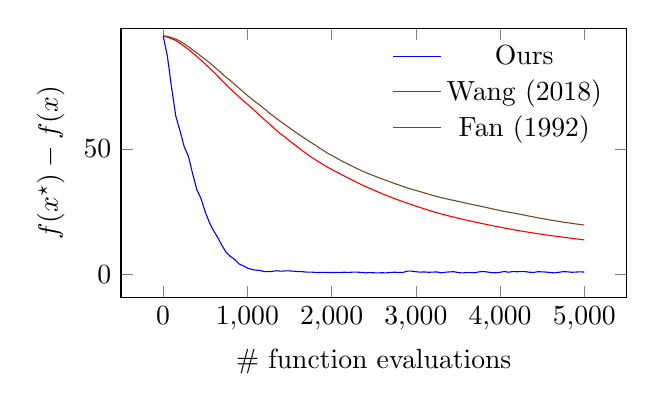
\begin{tikzpicture}
\begin{axis}[xlabel={\# function evaluations}, ylabel={$\lvert f(x^\star) - f(x) \rvert$}, width={8cm}, height={5cm}, ymax={98}, legend style={draw=none, fill=none}]
    \legend{{Ours},{Wang (2018)},{Fan (1992)}}
    \addplot+[no marks]
        table[row sep={\\}]
        {
            x  y  \\
            0.0  95.0  \\
            50.0  86.92688506338338  \\
            100.0  74.48395541925407  \\
            150.0  63.07666999954801  \\
            200.0  57.2607038503202  \\
            250.0  50.908833958660246  \\
            300.0  47.10146987100649  \\
            350.0  40.17122103123221  \\
            400.0  33.79924172687648  \\
            450.0  30.234129561848825  \\
            500.0  24.92030144424448  \\
            550.0  20.731718201964277  \\
            600.0  17.4334891945042  \\
            650.0  14.690871360980669  \\
            700.0  11.525266188442675  \\
            750.0  8.782131858275214  \\
            800.0  7.23765563663222  \\
            850.0  6.053575750504545  \\
            900.0  4.319878463569948  \\
            950.0  3.552785285314473  \\
            1000.0  2.668191277157813  \\
            1050.0  2.087978766109882  \\
            1100.0  1.8097797293656475  \\
            1150.0  1.7057423380337624  \\
            1200.0  1.2024016767168526  \\
            1250.0  1.2134766738379277  \\
            1300.0  1.3551026692913828  \\
            1350.0  1.5635914257744015  \\
            1400.0  1.404038562425725  \\
            1450.0  1.512283826130773  \\
            1500.0  1.5180532713553536  \\
            1550.0  1.3989922703863886  \\
            1600.0  1.2556566667098634  \\
            1650.0  1.2139158531453882  \\
            1700.0  1.0405147850440668  \\
            1750.0  1.0470667775136406  \\
            1800.0  0.9313196620360611  \\
            1850.0  0.8743063094119456  \\
            1900.0  0.9541325225539842  \\
            1950.0  0.8783816132947954  \\
            2000.0  0.8727423952079403  \\
            2050.0  0.9037082675249946  \\
            2100.0  0.8869478685181305  \\
            2150.0  0.9913760280049109  \\
            2200.0  0.8990486859019684  \\
            2250.0  1.0080073584876033  \\
            2300.0  1.0209423136328748  \\
            2350.0  0.907666791260809  \\
            2400.0  0.7312598769356763  \\
            2450.0  0.8679083941437422  \\
            2500.0  0.7590607390870661  \\
            2550.0  0.7292420352119223  \\
            2600.0  0.7749656655331819  \\
            2650.0  0.7322116128422672  \\
            2700.0  0.8850065602876098  \\
            2750.0  0.9995300483307634  \\
            2800.0  0.8657456861322033  \\
            2850.0  0.9276509632416583  \\
            2900.0  1.4162343589298851  \\
            2950.0  1.4340810970916464  \\
            3000.0  1.1807846700613411  \\
            3050.0  1.0264271234707196  \\
            3100.0  1.0982306242872113  \\
            3150.0  0.9675508739319226  \\
            3200.0  1.0167309760833203  \\
            3250.0  1.1038087888726797  \\
            3300.0  0.7483631119340992  \\
            3350.0  0.9778302145304075  \\
            3400.0  1.1132164227925976  \\
            3450.0  1.1944052522295425  \\
            3500.0  0.8529276342316756  \\
            3550.0  0.710275842698898  \\
            3600.0  0.8327029803277262  \\
            3650.0  0.8012208006929805  \\
            3700.0  0.7956460455884145  \\
            3750.0  1.1253822951711576  \\
            3800.0  1.3010902280381822  \\
            3850.0  1.0619714830000746  \\
            3900.0  0.817579333700858  \\
            3950.0  0.7796747596219149  \\
            4000.0  0.9604939131472778  \\
            4050.0  1.266741850661171  \\
            4100.0  0.9918111722966796  \\
            4150.0  1.2476356065932903  \\
            4200.0  1.1823151029391459  \\
            4250.0  1.2479199517869493  \\
            4300.0  1.1990574763359527  \\
            4350.0  0.9812884284147885  \\
            4400.0  0.9160726977035565  \\
            4450.0  1.1998597224934537  \\
            4500.0  1.1310133116061323  \\
            4550.0  1.0383634927460788  \\
            4600.0  0.8360838849396007  \\
            4650.0  0.7345156363149569  \\
            4700.0  0.9623472827785953  \\
            4750.0  1.2147337554275535  \\
            4800.0  1.1451648454907517  \\
            4850.0  0.9726710357680879  \\
            4900.0  1.0485780728558904  \\
            4950.0  1.1513046881730973  \\
            5000.0  1.041458912077812  \\
        }
        ;
    \addplot+[no marks]
        table[row sep={\\}]
        {
            x  y  \\
            0.0  95.0  \\
            50.0  94.45200407797681  \\
            100.0  93.85071857150601  \\
            150.0  93.12666489036995  \\
            200.0  92.00150890852889  \\
            250.0  90.87511861279825  \\
            300.0  89.6032479584178  \\
            350.0  88.18868388361417  \\
            400.0  86.77817811957738  \\
            450.0  85.34043316240255  \\
            500.0  83.74418358671826  \\
            550.0  82.13328065766962  \\
            600.0  80.59698885319995  \\
            650.0  78.86592738091638  \\
            700.0  77.15872062303356  \\
            750.0  75.38874158057942  \\
            800.0  73.7938993706989  \\
            850.0  72.26049857738177  \\
            900.0  70.7230933098338  \\
            950.0  69.25175399004395  \\
            1000.0  67.7970051424959  \\
            1050.0  66.33808178600232  \\
            1100.0  64.79425824102859  \\
            1150.0  63.26684629540381  \\
            1200.0  61.74543449113505  \\
            1250.0  60.250239895240355  \\
            1300.0  58.77228457189068  \\
            1350.0  57.251035755688164  \\
            1400.0  55.891108539119344  \\
            1450.0  54.61176115174702  \\
            1500.0  53.23873037321646  \\
            1550.0  51.98179372384748  \\
            1600.0  50.664603862471424  \\
            1650.0  49.35449567339586  \\
            1700.0  48.18964553143103  \\
            1750.0  46.979155238295625  \\
            1800.0  45.87767649260961  \\
            1850.0  44.79968712207235  \\
            1900.0  43.773925729080666  \\
            1950.0  42.78847594447637  \\
            2000.0  41.89891759608961  \\
            2050.0  41.00935223360584  \\
            2100.0  40.13993906765961  \\
            2150.0  39.25660595085529  \\
            2200.0  38.385000613722724  \\
            2250.0  37.557129866912106  \\
            2300.0  36.69624804933529  \\
            2350.0  35.883546042961925  \\
            2400.0  35.09916651199926  \\
            2450.0  34.3668255140413  \\
            2500.0  33.64518289377117  \\
            2550.0  32.93317256307173  \\
            2600.0  32.21690975484487  \\
            2650.0  31.532342288625713  \\
            2700.0  30.86918531702486  \\
            2750.0  30.211417907907265  \\
            2800.0  29.606985398099663  \\
            2850.0  28.998656153279185  \\
            2900.0  28.416791930583717  \\
            2950.0  27.836745600939825  \\
            3000.0  27.279341191573245  \\
            3050.0  26.726608706582642  \\
            3100.0  26.176482255457646  \\
            3150.0  25.65781463384676  \\
            3200.0  25.142176518024634  \\
            3250.0  24.65287486507048  \\
            3300.0  24.183415055462017  \\
            3350.0  23.738013151905033  \\
            3400.0  23.309292766969662  \\
            3450.0  22.893573445715823  \\
            3500.0  22.477399812324666  \\
            3550.0  22.080195766144303  \\
            3600.0  21.700011275882048  \\
            3650.0  21.333362614696668  \\
            3700.0  20.967571251837224  \\
            3750.0  20.607341960671935  \\
            3800.0  20.254601951530855  \\
            3850.0  19.909838226233727  \\
            3900.0  19.563883265029407  \\
            3950.0  19.224457311013715  \\
            4000.0  18.907008677459267  \\
            4050.0  18.5761451928444  \\
            4100.0  18.266985583340407  \\
            4150.0  17.957087290172073  \\
            4200.0  17.656338651715902  \\
            4250.0  17.373695825589607  \\
            4300.0  17.0959107652407  \\
            4350.0  16.815903529445933  \\
            4400.0  16.55703367553761  \\
            4450.0  16.294126107694655  \\
            4500.0  16.045158795123022  \\
            4550.0  15.801831211045615  \\
            4600.0  15.566743396909672  \\
            4650.0  15.34474028941614  \\
            4700.0  15.132502429387044  \\
            4750.0  14.912856977611396  \\
            4800.0  14.690770172531337  \\
            4850.0  14.4721592929037  \\
            4900.0  14.260094758472475  \\
            4950.0  14.048749527643475  \\
            5000.0  13.840192402082208  \\
        }
        ;
    \addplot+[no marks]
        table[row sep={\\}]
        {
            x  y  \\
            0.0  95.0  \\
            50.0  94.7592034562115  \\
            100.0  94.27486182912651  \\
            150.0  93.65545899095565  \\
            200.0  92.85543625258572  \\
            250.0  91.81865635766707  \\
            300.0  90.66371527984252  \\
            350.0  89.40748926033363  \\
            400.0  88.18816191370296  \\
            450.0  86.87770680651201  \\
            500.0  85.60956830257884  \\
            550.0  84.3262601139828  \\
            600.0  82.86416451271796  \\
            650.0  81.43468676379878  \\
            700.0  79.9460828299247  \\
            750.0  78.38141514339573  \\
            800.0  77.13401129049551  \\
            850.0  75.65707341702503  \\
            900.0  74.20583123724833  \\
            950.0  72.73901895062052  \\
            1000.0  71.24276365281531  \\
            1050.0  69.95985923912873  \\
            1100.0  68.61241862909714  \\
            1150.0  67.359720961404  \\
            1200.0  66.02945111385542  \\
            1250.0  64.6069869994266  \\
            1300.0  63.28420097054796  \\
            1350.0  62.02463795715612  \\
            1400.0  60.78989136267625  \\
            1450.0  59.61595062184901  \\
            1500.0  58.3785352960116  \\
            1550.0  57.20683481363261  \\
            1600.0  56.02213164385147  \\
            1650.0  54.898274441882684  \\
            1700.0  53.813024996672326  \\
            1750.0  52.714668990155076  \\
            1800.0  51.617752646323446  \\
            1850.0  50.53936376029601  \\
            1900.0  49.43760676015783  \\
            1950.0  48.34674835753407  \\
            2000.0  47.46237649189291  \\
            2050.0  46.52445293362856  \\
            2100.0  45.59822391565341  \\
            2150.0  44.7039962599492  \\
            2200.0  43.89949428816642  \\
            2250.0  43.05402871779469  \\
            2300.0  42.23504407326578  \\
            2350.0  41.43124002532861  \\
            2400.0  40.70379217197582  \\
            2450.0  39.966438757944495  \\
            2500.0  39.36401503503258  \\
            2550.0  38.68129860472375  \\
            2600.0  38.070748067767795  \\
            2650.0  37.46430902385679  \\
            2700.0  36.84191567926455  \\
            2750.0  36.23940611720972  \\
            2800.0  35.641042971773835  \\
            2850.0  35.074006604340994  \\
            2900.0  34.49572625852925  \\
            2950.0  33.99997320889723  \\
            3000.0  33.51839895120941  \\
            3050.0  33.02691697966133  \\
            3100.0  32.54449175563856  \\
            3150.0  32.03889904884239  \\
            3200.0  31.553100002606346  \\
            3250.0  31.057467172384577  \\
            3300.0  30.66364923625832  \\
            3350.0  30.278585336945074  \\
            3400.0  29.87753858328534  \\
            3450.0  29.540307182512763  \\
            3500.0  29.18820755650187  \\
            3550.0  28.809592580870312  \\
            3600.0  28.426238703011943  \\
            3650.0  28.062691761589473  \\
            3700.0  27.67570873750112  \\
            3750.0  27.355730844740037  \\
            3800.0  27.007744735432762  \\
            3850.0  26.638958737566746  \\
            3900.0  26.254686235399248  \\
            3950.0  25.87140548772112  \\
            4000.0  25.52271724588555  \\
            4050.0  25.163040044460182  \\
            4100.0  24.86869220546485  \\
            4150.0  24.587239054239458  \\
            4200.0  24.264322014253246  \\
            4250.0  23.94046607879286  \\
            4300.0  23.6088081137752  \\
            4350.0  23.268563806495287  \\
            4400.0  22.938141301434634  \\
            4450.0  22.606192580361757  \\
            4500.0  22.29579618181944  \\
            4550.0  22.029087760114763  \\
            4600.0  21.7222177437809  \\
            4650.0  21.449551126790173  \\
            4700.0  21.167489257495284  \\
            4750.0  20.889392866826178  \\
            4800.0  20.665917664766056  \\
            4850.0  20.4213186653504  \\
            4900.0  20.1836410043168  \\
            4950.0  19.97209423059016  \\
            5000.0  19.72951764902478  \\
        }
        ;
\end{axis}
\end{tikzpicture}

    \end{subfigure}%
    \hfill
    \begin{subfigure}[t]{1.\linewidth}
        \centering
        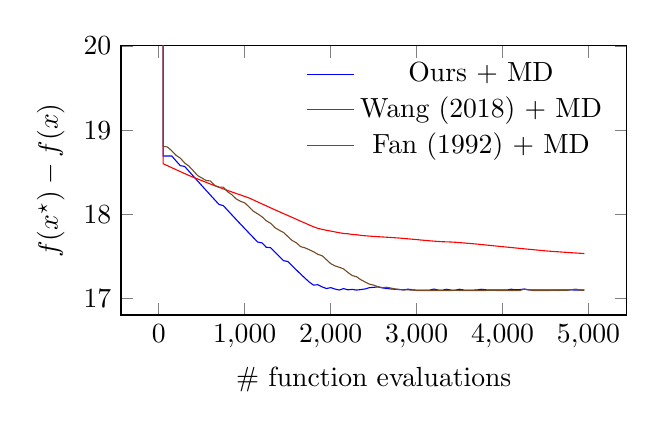
\begin{tikzpicture}
\begin{axis}[xlabel={\# function evaluations}, ylabel={$\lvert f(x^\star) - f(x) \rvert$}, width={8cm}, height={5cm}, ymax={20}, legend style={draw=none, fill=none}]
    \legend{{Ours + MD},{Wang (2018) + MD},{Fan (1992) + MD}}
    \addplot+[no marks]
        table[row sep={\\}]
        {
            x  y  \\
            1.0  95.0  \\
            51.0  18.693069188164465  \\
            101.0  18.69306128719503  \\
            151.0  18.693234354122385  \\
            201.0  18.634923000699505  \\
            251.0  18.577956645425235  \\
            301.0  18.56948979462798  \\
            351.0  18.51220284385783  \\
            401.0  18.45531108554571  \\
            451.0  18.39814377948552  \\
            501.0  18.341378494389502  \\
            551.0  18.284877205665687  \\
            601.0  18.2289702429745  \\
            651.0  18.173328463199486  \\
            701.0  18.117759974452248  \\
            751.0  18.1040990356649  \\
            801.0  18.048696660005888  \\
            851.0  17.993778671456067  \\
            901.0  17.93917284036985  \\
            951.0  17.885013312949322  \\
            1001.0  17.831133607614046  \\
            1051.0  17.777496260047055  \\
            1101.0  17.72431376639125  \\
            1151.0  17.671499338984688  \\
            1201.0  17.66210550427034  \\
            1251.0  17.60991143305378  \\
            1301.0  17.6053693220825  \\
            1351.0  17.553519837960035  \\
            1401.0  17.502209003238725  \\
            1451.0  17.451242244598316  \\
            1501.0  17.441246892680095  \\
            1551.0  17.390938416326122  \\
            1601.0  17.3412563062127  \\
            1651.0  17.291980860686735  \\
            1701.0  17.2438686205903  \\
            1751.0  17.19743703754484  \\
            1801.0  17.160772048559032  \\
            1851.0  17.165665049526442  \\
            1901.0  17.13956580777475  \\
            1951.0  17.12049012232302  \\
            2001.0  17.131213624196544  \\
            2051.0  17.11404795753296  \\
            2101.0  17.10242348577815  \\
            2151.0  17.119851146698238  \\
            2201.0  17.10502054888923  \\
            2251.0  17.110412327364553  \\
            2301.0  17.102014613369192  \\
            2351.0  17.10815503532697  \\
            2401.0  17.11552829623548  \\
            2451.0  17.130817706683384  \\
            2501.0  17.134679452456552  \\
            2551.0  17.140021241881055  \\
            2601.0  17.128092876304137  \\
            2651.0  17.121156703303946  \\
            2701.0  17.115308137975994  \\
            2751.0  17.111208048899314  \\
            2801.0  17.10811094428974  \\
            2851.0  17.105030638242773  \\
            2901.0  17.113020625754125  \\
            2951.0  17.104634155297138  \\
            3001.0  17.101294588899737  \\
            3051.0  17.10121549277203  \\
            3101.0  17.101229815757133  \\
            3151.0  17.101202087848474  \\
            3201.0  17.114157031658785  \\
            3251.0  17.102441883361738  \\
            3301.0  17.101415765624168  \\
            3351.0  17.11131587395418  \\
            3401.0  17.10171845673334  \\
            3451.0  17.10160644362613  \\
            3501.0  17.111535298387448  \\
            3551.0  17.102019920273047  \\
            3601.0  17.101812962486637  \\
            3651.0  17.101772067908158  \\
            3701.0  17.10308866676205  \\
            3751.0  17.111649376424925  \\
            3801.0  17.10555415002385  \\
            3851.0  17.10269658229593  \\
            3901.0  17.10264383748636  \\
            3951.0  17.102603040434023  \\
            4001.0  17.102556609013565  \\
            4051.0  17.102495556852535  \\
            4101.0  17.112257950349697  \\
            4151.0  17.105218221407828  \\
            4201.0  17.10850979288045  \\
            4251.0  17.113719909463388  \\
            4301.0  17.105172431299188  \\
            4351.0  17.104110882441176  \\
            4401.0  17.104053098289803  \\
            4451.0  17.104011158063493  \\
            4501.0  17.103952566338215  \\
            4551.0  17.10392193791994  \\
            4601.0  17.103866856840305  \\
            4651.0  17.103800203096206  \\
            4701.0  17.103752023893666  \\
            4751.0  17.103701685065964  \\
            4801.0  17.103652700074186  \\
            4851.0  17.103600594957523  \\
            4901.0  17.1035527401808  \\
            4951.0  17.104879138749943  \\
        }
        ;
    \addplot+[no marks]
        table[row sep={\\}]
        {
            x  y  \\
            1.0  95.0  \\
            51.0  18.60105076192452  \\
            101.0  18.57756642998254  \\
            151.0  18.55415173076179  \\
            201.0  18.530805503048924  \\
            251.0  18.507541935637246  \\
            301.0  18.48435444972855  \\
            351.0  18.461776103087008  \\
            401.0  18.440698044553198  \\
            451.0  18.42049205805403  \\
            501.0  18.400350666446002  \\
            551.0  18.380281174513133  \\
            601.0  18.36028829377156  \\
            651.0  18.340369022129906  \\
            701.0  18.321059319535145  \\
            751.0  18.302387367063286  \\
            801.0  18.28382787839281  \\
            851.0  18.265915106748583  \\
            901.0  18.248070454971334  \\
            951.0  18.230295233025323  \\
            1001.0  18.21258057555975  \\
            1051.0  18.194931725200895  \\
            1101.0  18.171284170636117  \\
            1151.0  18.147726138782154  \\
            1201.0  18.124338148700446  \\
            1251.0  18.10110595068009  \\
            1301.0  18.077931520426674  \\
            1351.0  18.0548422608681  \\
            1401.0  18.03213113957002  \\
            1451.0  18.009649359945875  \\
            1501.0  17.98723879198027  \\
            1551.0  17.964899365804637  \\
            1601.0  17.941982471105753  \\
            1651.0  17.919324745872437  \\
            1701.0  17.89688448399564  \\
            1751.0  17.874655401612678  \\
            1801.0  17.852822152645548  \\
            1851.0  17.834096960066397  \\
            1901.0  17.822488502648646  \\
            1951.0  17.81144256222563  \\
            2001.0  17.801951547284418  \\
            2051.0  17.791797678530052  \\
            2101.0  17.78248768217828  \\
            2151.0  17.7735177447794  \\
            2201.0  17.76987650330877  \\
            2251.0  17.761968244849065  \\
            2301.0  17.75866754667712  \\
            2351.0  17.75126107484895  \\
            2401.0  17.746480235833214  \\
            2451.0  17.74223035056705  \\
            2501.0  17.7388829590689  \\
            2551.0  17.73559994792227  \\
            2601.0  17.732347730086573  \\
            2651.0  17.729147601594974  \\
            2701.0  17.725979139075385  \\
            2751.0  17.722638735509328  \\
            2801.0  17.71892077613814  \\
            2851.0  17.71463723677139  \\
            2901.0  17.710107630395516  \\
            2951.0  17.705567816193952  \\
            3001.0  17.701097145736778  \\
            3051.0  17.695903186236592  \\
            3101.0  17.691411961995545  \\
            3151.0  17.686987123076506  \\
            3201.0  17.68265456715966  \\
            3251.0  17.678991205920003  \\
            3301.0  17.67576719716238  \\
            3351.0  17.674072696549455  \\
            3401.0  17.672421256095223  \\
            3451.0  17.66926080126744  \\
            3501.0  17.66506567329371  \\
            3551.0  17.660738679803423  \\
            3601.0  17.656452321690693  \\
            3651.0  17.65217979654662  \\
            3701.0  17.647934273430604  \\
            3751.0  17.64271365991345  \\
            3801.0  17.63750706484459  \\
            3851.0  17.63232671370166  \\
            3901.0  17.627160532706764  \\
            3951.0  17.622032896348536  \\
            4001.0  17.616923734226106  \\
            4051.0  17.61183646909738  \\
            4101.0  17.606773064543635  \\
            4151.0  17.601754808535123  \\
            4201.0  17.59669930686828  \\
            4251.0  17.59173181964737  \\
            4301.0  17.586761452227968  \\
            4351.0  17.58183773220329  \\
            4401.0  17.57695861773078  \\
            4451.0  17.572012454060975  \\
            4501.0  17.567283907069957  \\
            4551.0  17.56308143840007  \\
            4601.0  17.559511754620363  \\
            4651.0  17.55596053138021  \\
            4701.0  17.552433615935318  \\
            4751.0  17.5489294097366  \\
            4801.0  17.545445672099493  \\
            4851.0  17.54198654677248  \\
            4901.0  17.538714736975972  \\
            4951.0  17.535853504038236  \\
        }
        ;
    \addplot+[no marks]
        table[row sep={\\}]
        {
            x  y  \\
            1.0  95.0  \\
            51.0  18.80789710235338  \\
            101.0  18.79937582288313  \\
            151.0  18.754882244277006  \\
            201.0  18.700972952737377  \\
            251.0  18.666943980727183  \\
            301.0  18.610618013370058  \\
            351.0  18.572594049845645  \\
            401.0  18.51832501029947  \\
            451.0  18.461641835574003  \\
            501.0  18.431916706640685  \\
            551.0  18.401998627871944  \\
            601.0  18.396483176037997  \\
            651.0  18.344003158567276  \\
            701.0  18.323579864106822  \\
            751.0  18.323872558241213  \\
            801.0  18.26897170204648  \\
            851.0  18.23290354721995  \\
            901.0  18.183508426443275  \\
            951.0  18.1554395247647  \\
            1001.0  18.136441950833174  \\
            1051.0  18.08869509524899  \\
            1101.0  18.038029059395058  \\
            1151.0  18.006491543501443  \\
            1201.0  17.97193733159959  \\
            1251.0  17.92421178396923  \\
            1301.0  17.894961632384472  \\
            1351.0  17.843227661898656  \\
            1401.0  17.812440230108606  \\
            1451.0  17.785980774939677  \\
            1501.0  17.73812141061193  \\
            1551.0  17.690333429366074  \\
            1601.0  17.66319953404495  \\
            1651.0  17.61733665543734  \\
            1701.0  17.603281500682222  \\
            1751.0  17.580874139564372  \\
            1801.0  17.55657497575879  \\
            1851.0  17.525890112647886  \\
            1901.0  17.509727198076487  \\
            1951.0  17.462556982635068  \\
            2001.0  17.415298094669147  \\
            2051.0  17.388659185636065  \\
            2101.0  17.37231898694184  \\
            2151.0  17.352896272251332  \\
            2201.0  17.310661271573373  \\
            2251.0  17.27417100244417  \\
            2301.0  17.26051860626095  \\
            2351.0  17.224975421889187  \\
            2401.0  17.19835423393521  \\
            2451.0  17.172636285323566  \\
            2501.0  17.16041458787766  \\
            2551.0  17.142084633870297  \\
            2601.0  17.130632131413126  \\
            2651.0  17.13560418765785  \\
            2701.0  17.125703339666053  \\
            2751.0  17.115638072391086  \\
            2801.0  17.109120353482272  \\
            2851.0  17.103458972010152  \\
            2901.0  17.104371824743158  \\
            2951.0  17.101519275583936  \\
            3001.0  17.09741433960582  \\
            3051.0  17.097216947806615  \\
            3101.0  17.097153257054153  \\
            3151.0  17.097181699692975  \\
            3201.0  17.09717422646611  \\
            3251.0  17.0971736093486  \\
            3301.0  17.097179498057294  \\
            3351.0  17.097137306119738  \\
            3401.0  17.097103319090728  \\
            3451.0  17.098595073397107  \\
            3501.0  17.09708480051117  \\
            3551.0  17.097463847747328  \\
            3601.0  17.09707426666605  \\
            3651.0  17.097077721036758  \\
            3701.0  17.09710139998924  \\
            3751.0  17.097115291492678  \\
            3801.0  17.097076931219835  \\
            3851.0  17.099933141771636  \\
            3901.0  17.097798641475872  \\
            3951.0  17.09759649065479  \\
            4001.0  17.096966076316512  \\
            4051.0  17.09699969094766  \\
            4101.0  17.097022132438838  \\
            4151.0  17.097010178263165  \\
            4201.0  17.097045436047345  \\
            4251.0  17.114165231636697  \\
            4301.0  17.10561150361374  \\
            4351.0  17.096934329029725  \\
            4401.0  17.097004289573235  \\
            4451.0  17.09726496936708  \\
            4501.0  17.097689431477217  \\
            4551.0  17.097404148506232  \\
            4601.0  17.099026586764875  \\
            4651.0  17.09727955542028  \\
            4701.0  17.10044890373308  \\
            4751.0  17.098757170652878  \\
            4801.0  17.10586661584989  \\
            4851.0  17.11343773335606  \\
            4901.0  17.100756104893865  \\
            4951.0  17.098256463449818  \\
        }
        ;
\end{axis}
\end{tikzpicture}

    \end{subfigure}%
    \caption{Nesterov Gradient Descent (top) and Mirror Gradient Descent (bottom) on the Rosenbrock function for $d=100$.}\label{fig:rosenbrock_vs}
\end{figure}
We apply the previous method to the minimization of the log-likelihood of a logistic model on the UCI's Adult data set, consisting of $48842$ observations and $14$ attributes amounting to $101$ dimensions once one-hot encoded and an intercept added.
\begin{multline}
    \mathcal{L}_\theta (X) =  -\sum_i Y_i \log (1 + \exp (-\theta X_i)) \\
    -(1 - Y_i) \log (1 + \exp (\theta X_i)), \; \theta \in \mathbb{R}^{101}.
\end{multline}
We also compare the effective CPU wall time needed to reach a given log-likelihood in order to give a more comprehensive view of the relative performance of the multiple algorithms. Given that the time per iteration can vary greatly depending on the cost of evaluations and the cost of the gradient procedures, it is important to use both the number of evaluations and the time metric jointly with the former being more relevant as the cost of individual function evaluations increases.
\begin{figure}
    \centering
    \begin{subfigure}[b]{1.\linewidth}
        \centering
        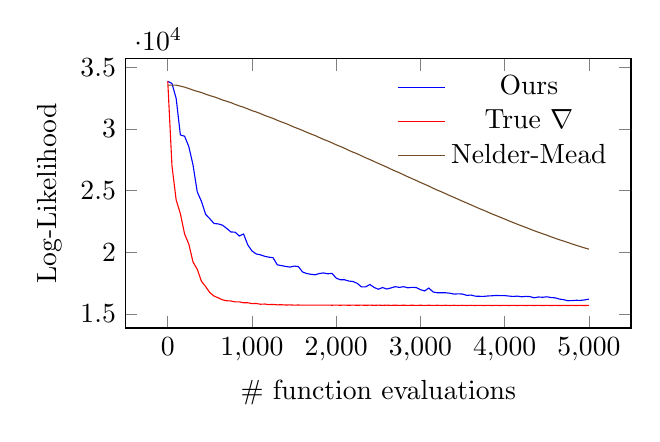
\begin{tikzpicture}
\begin{axis}[xlabel={\# function evaluations}, ylabel={Log-Likelihood},width=8cm,height=5cm, legend style={draw=none, fill=none}]
    \legend{{Ours},{True $\nabla$},{Nelder-Mead}}
    \addplot+[no marks]
        table[x expr=\thisrowno{0}*50, row sep={\\}]
        {
            x  y  \\
            0.0  33854.69459290893  \\
            1.0  33677.22039939559  \\
            2.0  32458.034543424343  \\
            3.0  29504.292538807375  \\
            4.0  29401.98595996619  \\
            5.0  28566.099881137026  \\
            6.0  27077.210306102214  \\
            7.0  24899.568114719965  \\
            8.0  24122.619090449403  \\
            9.0  23071.730482166917  \\
            10.0  22713.105395963452  \\
            11.0  22325.889712367858  \\
            12.0  22300.212635690026  \\
            13.0  22193.619216193416  \\
            14.0  21932.02247412401  \\
            15.0  21646.115993838666  \\
            16.0  21628.94697815015  \\
            17.0  21315.511598604964  \\
            18.0  21482.84844699411  \\
            19.0  20602.114174475642  \\
            20.0  20103.178128264455  \\
            21.0  19864.190264148187  \\
            22.0  19796.248585720106  \\
            23.0  19675.999380276524  \\
            24.0  19602.387719331662  \\
            25.0  19565.216845965617  \\
            26.0  18985.16072347002  \\
            27.0  18921.494795565886  \\
            28.0  18852.287189024253  \\
            29.0  18800.25164343183  \\
            30.0  18877.63190785741  \\
            31.0  18847.26953697681  \\
            32.0  18405.275048964566  \\
            33.0  18277.455142377043  \\
            34.0  18216.816680207314  \\
            35.0  18176.963775191794  \\
            36.0  18280.436047539886  \\
            37.0  18326.18000682086  \\
            38.0  18257.789544661748  \\
            39.0  18292.509018312805  \\
            40.0  17903.58767135723  \\
            41.0  17769.975809777796  \\
            42.0  17773.287310681662  \\
            43.0  17669.564120682167  \\
            44.0  17631.808370289385  \\
            45.0  17481.006859516063  \\
            46.0  17194.468858575136  \\
            47.0  17199.604304697365  \\
            48.0  17390.753876452098  \\
            49.0  17150.362181317203  \\
            50.0  17005.811725549058  \\
            51.0  17143.614781700344  \\
            52.0  17024.0556049907  \\
            53.0  17110.32213310158  \\
            54.0  17214.71497815532  \\
            55.0  17155.683873648595  \\
            56.0  17213.928837926207  \\
            57.0  17124.349404656954  \\
            58.0  17157.87937098154  \\
            59.0  17145.70333378915  \\
            60.0  16969.927940222373  \\
            61.0  16870.407162003023  \\
            62.0  17105.236185256457  \\
            63.0  16785.006544689713  \\
            64.0  16720.326214684  \\
            65.0  16717.07492916102  \\
            66.0  16718.694925923282  \\
            67.0  16683.640432761847  \\
            68.0  16611.379221321757  \\
            69.0  16633.92076169581  \\
            70.0  16615.151076368722  \\
            71.0  16509.527788427233  \\
            72.0  16535.25831025839  \\
            73.0  16444.248013317818  \\
            74.0  16434.774003939507  \\
            75.0  16427.81970083801  \\
            76.0  16459.270802711126  \\
            77.0  16477.126894204062  \\
            78.0  16499.870788100918  \\
            79.0  16489.49166335023  \\
            80.0  16488.06827303105  \\
            81.0  16453.61562471029  \\
            82.0  16423.671139699356  \\
            83.0  16448.04481969719  \\
            84.0  16396.745133488068  \\
            85.0  16426.382023806218  \\
            86.0  16408.660737148417  \\
            87.0  16313.262439616054  \\
            88.0  16377.835455719147  \\
            89.0  16353.787659629124  \\
            90.0  16393.876074713116  \\
            91.0  16332.9756146266  \\
            92.0  16308.715089409168  \\
            93.0  16207.86417774294  \\
            94.0  16159.484859636686  \\
            95.0  16076.133527803006  \\
            96.0  16084.971758077143  \\
            97.0  16112.307748533738  \\
            98.0  16103.349835735462  \\
            99.0  16142.928943866573  \\
            100.0  16204.72589768977  \\
        }
        ;
    \addplot+[no marks]
        table[x expr=\thisrowno{0}*50, row sep={\\}]
        {
            x  y  \\
            0.0  33854.69459290893  \\
            1.0  27002.376382826966  \\
            2.0  24235.673803400277  \\
            3.0  23118.9609567904  \\
            4.0  21485.09998757173  \\
            5.0  20663.150226737722  \\
            6.0  19206.69467601885  \\
            7.0  18625.581740616723  \\
            8.0  17650.472797312927  \\
            9.0  17218.916376489113  \\
            10.0  16725.582907923774  \\
            11.0  16453.299306404377  \\
            12.0  16308.713644813395  \\
            13.0  16145.324449186197  \\
            14.0  16072.896590809862  \\
            15.0  16054.605385079865  \\
            16.0  15977.01929884535  \\
            17.0  15987.332967269258  \\
            18.0  15906.491714899821  \\
            19.0  15914.25244301249  \\
            20.0  15841.382762559188  \\
            21.0  15851.633307335076  \\
            22.0  15791.742203760201  \\
            23.0  15807.42290183  \\
            24.0  15760.981273274614  \\
            25.0  15775.371569742772  \\
            26.0  15741.410448209326  \\
            27.0  15752.20938916564  \\
            28.0  15727.714542186148  \\
            29.0  15736.650551754281  \\
            30.0  15720.78873467609  \\
            31.0  15726.736426111762  \\
            32.0  15718.15718765758  \\
            33.0  15720.509945211143  \\
            34.0  15717.868971768283  \\
            35.0  15716.49184171433  \\
            36.0  15718.56709725128  \\
            37.0  15713.68325197482  \\
            38.0  15719.420213650672  \\
            39.0  15711.47035276341  \\
            40.0  15719.996033303563  \\
            41.0  15709.513483388448  \\
            42.0  15720.128784497061  \\
            43.0  15707.649587194803  \\
            44.0  15719.80909667506  \\
            45.0  15705.818482668128  \\
            46.0  15719.105233088576  \\
            47.0  15704.013101180502  \\
            48.0  15718.113307493986  \\
            49.0  15702.24908229371  \\
            50.0  15716.929535701714  \\
            51.0  15700.548008341588  \\
            52.0  15715.637148982767  \\
            53.0  15698.929296382397  \\
            54.0  15714.302027068159  \\
            55.0  15697.407094945167  \\
            56.0  15712.97293900666  \\
            57.0  15695.989796377893  \\
            58.0  15711.683843787141  \\
            59.0  15694.680736823393  \\
            60.0  15710.456819243856  \\
            61.0  15693.479299846624  \\
            62.0  15709.304899579918  \\
            63.0  15692.382033936934  \\
            64.0  15708.234516939463  \\
            65.0  15691.383617693911  \\
            66.0  15707.247464521195  \\
            67.0  15690.47762382601  \\
            68.0  15706.342405434483  \\
            69.0  15689.657088782622  \\
            70.0  15705.515994147958  \\
            71.0  15688.914917058477  \\
            72.0  15704.763687136216  \\
            73.0  15688.244154540891  \\
            74.0  15704.080313925579  \\
            75.0  15687.638162935069  \\
            76.0  15703.46046864584  \\
            77.0  15687.090722130864  \\
            78.0  15702.898770108439  \\
            79.0  15686.596081719996  \\
            80.0  15702.390027431691  \\
            81.0  15686.148977756518  \\
            82.0  15701.929339044387  \\
            83.0  15685.744626618949  \\
            84.0  15701.512145594443  \\
            85.0  15685.378704505849  \\
            86.0  15701.134251665373  \\
            87.0  15685.047318569828  \\
            88.0  15700.79182696977  \\
            89.0  15684.746973823067  \\
            90.0  15700.481394554132  \\
            91.0  15684.474538586532  \\
            92.0  15700.199811259903  \\
            93.0  15684.227210282863  \\
            94.0  15699.944244031192  \\
            95.0  15684.00248268868  \\
            96.0  15699.712144478071  \\
            97.0  15683.798115288486  \\
            98.0  15699.501223268373  \\
            99.0  15683.612105051503  \\
            100.0  15699.309425336454  \\
        }
        ;
    \addplot+[no marks]
        table[x expr=\thisrowno{0}*50, row sep={\\}]
        {
            x  y  \\
            0.0  33540.16027479392  \\
            1.0  33540.16027479392  \\
            2.0  33540.16027479392  \\
            3.0  33461.71527544366  \\
            4.0  33373.30722027231  \\
            5.0  33268.19095503645  \\
            6.0  33140.06436822765  \\
            7.0  33035.45733013374  \\
            8.0  32940.93090272498  \\
            9.0  32808.98356010157  \\
            10.0  32690.600326102798  \\
            11.0  32595.018964676543  \\
            12.0  32471.1116158417  \\
            13.0  32339.37378062083  \\
            14.0  32231.830036275507  \\
            15.0  32122.14222845474  \\
            16.0  31981.4472894099  \\
            17.0  31860.031829508614  \\
            18.0  31748.39332528856  \\
            19.0  31615.304172470995  \\
            20.0  31475.224573281073  \\
            21.0  31367.435004244122  \\
            22.0  31240.459748043162  \\
            23.0  31088.464423793474  \\
            24.0  30965.51162072635  \\
            25.0  30846.60149069171  \\
            26.0  30693.18093487493  \\
            27.0  30560.735306269486  \\
            28.0  30438.088319527436  \\
            29.0  30291.50447746284  \\
            30.0  30140.795574951197  \\
            31.0  30010.55356625044  \\
            32.0  29876.99224551849  \\
            33.0  29723.54669826969  \\
            34.0  29582.90552358378  \\
            35.0  29454.36820477756  \\
            36.0  29294.44069180391  \\
            37.0  29142.952672105723  \\
            38.0  29013.443766039156  \\
            39.0  28864.553602916312  \\
            40.0  28706.14074070978  \\
            41.0  28569.8311939267  \\
            42.0  28421.878208067516  \\
            43.0  28256.648630447216  \\
            44.0  28108.37679221311  \\
            45.0  27977.13775160098  \\
            46.0  27813.187092832384  \\
            47.0  27652.643047593723  \\
            48.0  27512.09574559861  \\
            49.0  27355.310798712653  \\
            50.0  27199.661641057643  \\
            51.0  27051.37581322994  \\
            52.0  26901.028646370814  \\
            53.0  26736.814687498132  \\
            54.0  26582.23974149898  \\
            55.0  26442.53910874368  \\
            56.0  26278.782825221555  \\
            57.0  26117.37389928144  \\
            58.0  25969.679531103353  \\
            59.0  25817.12717623395  \\
            60.0  25656.633342067427  \\
            61.0  25510.094490140233  \\
            62.0  25360.356139347186  \\
            63.0  25191.025543865482  \\
            64.0  25035.368031495214  \\
            65.0  24896.07837222572  \\
            66.0  24743.63457817628  \\
            67.0  24584.75981909888  \\
            68.0  24440.491894034905  \\
            69.0  24286.973507151903  \\
            70.0  24135.119739624664  \\
            71.0  23991.4784084509  \\
            72.0  23843.682000673038  \\
            73.0  23687.6779489477  \\
            74.0  23541.016146231334  \\
            75.0  23403.831103369997  \\
            76.0  23255.27665005737  \\
            77.0  23104.862361867523  \\
            78.0  22969.36083662811  \\
            79.0  22832.837102155943  \\
            80.0  22691.5352305085  \\
            81.0  22546.492287790505  \\
            82.0  22413.232969844696  \\
            83.0  22273.060015329545  \\
            84.0  22143.85561362165  \\
            85.0  22017.036697126976  \\
            86.0  21881.976555493842  \\
            87.0  21747.61299227213  \\
            88.0  21624.502623338292  \\
            89.0  21501.388305392713  \\
            90.0  21384.869621921913  \\
            91.0  21256.95719197518  \\
            92.0  21131.30647354067  \\
            93.0  21014.44273907754  \\
            94.0  20909.652576141783  \\
            95.0  20792.421153608026  \\
            96.0  20675.14453498669  \\
            97.0  20564.564971739266  \\
            98.0  20457.311343988215  \\
            99.0  20349.62101171397  \\
            100.0  20254.80390403644  \\
        }
        ;
\end{axis}
\end{tikzpicture}
 %
    \end{subfigure}%
    \vfill
    \begin{subfigure}[b]{1.\linewidth}
        \centering
        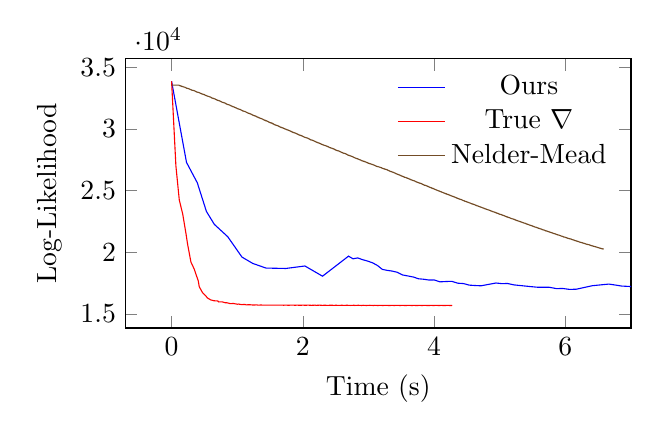
\begin{tikzpicture}
\begin{axis}[xlabel={Time (s)}, ylabel={Log-Likelihood}, width={8cm}, height={5cm}, legend style={draw=none, fill=none}, xmax={7}]
    \legend{{Ours},{True $\nabla$},{Nelder-Mead}}
    \addplot+[no marks]
        table[row sep={\\}]
        {
            x  y  \\
            0.0  33854.69459290893  \\
            0.227473239  27280.36763854949  \\
            0.391847711  25629.060209098363  \\
            0.530738634  23308.99722419768  \\
            0.651311315  22260.625231751  \\
            0.855261209  21263.18931223247  \\
            1.072547274  19609.955966986017  \\
            1.236480956  19097.59733114342  \\
            1.438516866  18720.75531564356  \\
            1.739630806  18688.196579031774  \\
            2.031406185  18889.6603648058  \\
            2.299805759  18062.888087497442  \\
            2.6960879  19687.1032616323  \\
            2.764134709  19472.594736258947  \\
            2.835652575  19542.4799130463  \\
            2.912244603  19397.437495005594  \\
            2.988574951  19284.788690666763  \\
            3.064703078  19139.97493302828  \\
            3.137132756  18926.9503359287  \\
            3.210671267  18614.9267617132  \\
            3.284335229  18534.83381744606  \\
            3.357079058  18480.039618487895  \\
            3.436658753  18382.992489068092  \\
            3.520436008  18161.82633246395  \\
            3.602754629  18079.264760190184  \\
            3.685610212  17992.599931292785  \\
            3.762503331  17852.722986346664  \\
            3.83941329  17816.73389032401  \\
            3.920549858  17751.50371378907  \\
            4.001641727  17759.550790309622  \\
            4.086907875  17605.46575197226  \\
            4.180834074  17631.51666117536  \\
            4.269275869  17648.224724258722  \\
            4.358478097  17496.154650939818  \\
            4.448706217  17464.494550716307  \\
            4.535738659  17337.651957807204  \\
            4.621270208  17308.484516006447  \\
            4.713825913  17284.35855410191  \\
            4.942815736  17510.3237251855  \\
            5.032267704  17459.58680954124  \\
            5.119090496  17471.959697326343  \\
            5.213981297  17359.00984820648  \\
            5.457543723  17226.677839761556  \\
            5.565978195  17171.40846065381  \\
            5.664266654  17168.202253089712  \\
            5.756790289  17162.881480424934  \\
            5.861569593  17059.35880123311  \\
            5.965623815  17064.013654998904  \\
            6.063106322  16992.569260634824  \\
            6.16561647  17007.645251374925  \\
            6.412651965  17293.882975894074  \\
            6.661785544  17423.7749015262  \\
            6.758517189  17348.408331105566  \\
            6.856315806  17263.82305806556  \\
            6.97384812  17231.21868635218  \\
            7.074275603  17197.366593393454  \\
            7.177247583  17223.421596848915  \\
            7.462121115  17232.862891227123  \\
            7.563816222  17158.001117414555  \\
            7.665304898  17090.694994407044  \\
            7.768706278  17036.33832642097  \\
            8.032359052  17009.518772607575  \\
            8.136215873  17060.32760988622  \\
            8.240643456  17006.11789199266  \\
            8.361555497  16986.587247243693  \\
            8.467089383  16927.658996200247  \\
            8.580132596  16917.447534858587  \\
            8.709063576  16872.54264571511  \\
            8.815592873  16806.06132442079  \\
            8.922688722  16756.796621418493  \\
            9.02892786  16764.1150846965  \\
            9.148456597  16728.88770313054  \\
            9.26981965  16796.99719258148  \\
            9.600451309  16823.323770401836  \\
            9.915218451  16807.65435385111  \\
            10.03534621  16635.556221836836  \\
            10.153928676  16641.334720596176  \\
            10.277851014  16645.496353318485  \\
            10.393918594  16581.145084126496  \\
            10.506305266  16637.823715265367  \\
            10.637855522  16609.512346623163  \\
            10.923794447  16713.41135631378  \\
            11.21743366  16906.483972164766  \\
            11.487525148  16814.70614304475  \\
            11.799359793  16770.528508510313  \\
            12.262230189  16838.46176669757  \\
            12.70079746  16857.294852410658  \\
            13.045453761  16750.698763736225  \\
            13.437535063  16599.38905352924  \\
            13.944185961  16629.959845984966  \\
            14.333458917  16711.82119847568  \\
            14.632608243  16653.163246617652  \\
            14.935573457  16660.595108221387  \\
            15.224215339  16567.105359867786  \\
            15.348727748  16567.69122015029  \\
            15.47413428  16574.951289979188  \\
            15.62024881  16615.83428191816  \\
            15.749128649  16528.559852264578  \\
            15.875978424  16520.50217391806  \\
            16.001881707  16578.660613388023  \\
            16.143200676  16536.7933394875  \\
        }
        ;
    \addplot+[no marks]
        table[row sep={\\}]
        {
            x  y  \\
            0.0  33854.69459290893  \\
            0.065708472  27002.376382826966  \\
            0.117270422  24235.673803400277  \\
            0.168641702  23118.960956790397  \\
            0.220138282  21485.09998757173  \\
            0.243632546  20663.150226737722  \\
            0.294706305  19206.69467601885  \\
            0.346154865  18625.58174061672  \\
            0.407998579  17650.472797312923  \\
            0.420760158  17218.916376489113  \\
            0.471749127  16725.582907923774  \\
            0.523449997  16453.299306404377  \\
            0.543713554  16308.7136448134  \\
            0.594982554  16145.324449186195  \\
            0.646763374  16072.89659080986  \\
            0.7050608  16054.605385079867  \\
            0.717537619  15977.01929884535  \\
            0.769208959  15987.33296726926  \\
            0.82122302  15906.491714899821  \\
            0.841338076  15914.252443012487  \\
            0.892700846  15841.382762559188  \\
            0.944133436  15851.633307335076  \\
            1.00216049  15791.742203760201  \\
            1.01466547  15807.42290183  \\
            1.066126679  15760.981273274612  \\
            1.117695659  15775.37156974277  \\
            1.138046557  15741.410448209328  \\
            1.189099095  15752.209389165648  \\
            1.240217654  15727.714542186148  \\
            1.299212411  15736.650551754285  \\
            1.311732591  15720.788734676094  \\
            1.363405141  15726.736426111758  \\
            1.41489885  15718.157187657587  \\
            1.434993977  15720.509945211146  \\
            1.486124566  15717.868971768286  \\
            1.537287925  15716.491841714329  \\
            1.595725391  15718.56709725128  \\
            1.607930479  15713.68325197482  \\
            1.659462479  15719.420213650668  \\
            1.711009769  15711.470352763408  \\
            1.731060836  15719.996033303567  \\
            1.782352435  15709.513483388444  \\
            1.833904675  15720.12878449706  \\
            1.892424691  15707.649587194805  \\
            1.90496499  15719.809096675059  \\
            1.95643642  15705.818482668132  \\
            2.00794882  15719.105233088576  \\
            2.027961306  15704.013101180502  \\
            2.078916615  15718.113307493986  \\
            2.130521435  15702.249082293712  \\
            2.188940311  15716.929535701713  \\
            2.20149648  15700.548008341588  \\
            2.252715339  15715.637148982769  \\
            2.304207199  15698.929296382394  \\
            2.324637886  15714.302027068157  \\
            2.375699965  15697.407094945167  \\
            2.427000054  15712.97293900666  \\
            2.484765929  15695.989796377895  \\
            2.497140138  15711.683843787143  \\
            2.548388017  15694.680736823393  \\
            2.599650856  15710.456819243856  \\
            2.619629202  15693.479299846622  \\
            2.670646031  15709.304899579916  \\
            2.72180763  15692.382033936936  \\
            2.780102686  15708.234516939463  \\
            2.792538545  15691.383617693915  \\
            2.843519483  15707.247464521195  \\
            2.894936103  15690.47762382601  \\
            2.916751414  15706.342405434487  \\
            2.968057993  15689.657088782626  \\
            3.019341932  15705.515994147956  \\
            3.077245797  15688.914917058479  \\
            3.089639046  15704.763687136216  \\
            3.140829485  15688.244154540891  \\
            3.192312774  15704.080313925582  \\
            3.212550182  15687.638162935069  \\
            3.264287722  15703.46046864584  \\
            3.315694671  15687.090722130863  \\
            3.373940327  15702.898770108442  \\
            3.386596226  15686.596081719994  \\
            3.437926036  15702.39002743169  \\
            3.489171275  15686.148977756518  \\
            3.509375892  15701.929339044385  \\
            3.561056052  15685.74462661895  \\
            3.612679512  15701.512145594443  \\
            3.670639117  15685.378704505845  \\
            3.682938006  15701.134251665377  \\
            3.734037044  15685.047318569834  \\
            3.785058423  15700.791826969767  \\
            3.804931239  15684.746973823068  \\
            3.856280319  15700.481394554132  \\
            3.907834719  15684.47453858653  \\
            3.966705925  15700.199811259903  \\
            3.979258745  15684.227210282865  \\
            4.030664034  15699.944244031194  \\
            4.082439185  15684.002482688678  \\
            4.10207982  15699.712144478071  \\
            4.15336928  15683.798115288486  \\
            4.204829279  15699.50122326837  \\
            4.262962935  15683.612105051507  \\
            4.275335083  15699.309425336454  \\
        }
        ;
    \addplot+[no marks]
        table[row sep={\\}]
        {
            x  y  \\
            9.5367431640625e-7  33540.16027479392  \\
            0.013138055801391602  33540.16027479392  \\
            0.014132022857666016  33540.16027479392  \\
            0.014842987060546875  33540.16027479392  \\
            0.015594959259033203  33540.16027479392  \\
            0.016288042068481445  33540.16027479392  \\
            0.01694011688232422  33540.16027479392  \\
            0.0176999568939209  33540.16027479392  \\
            0.018383026123046875  33540.16027479392  \\
            0.019025087356567383  33540.16027479392  \\
            0.019807100296020508  33540.16027479392  \\
            0.020591020584106445  33540.16027479392  \\
            0.02126908302307129  33540.16027479392  \\
            0.02191901206970215  33540.16027479392  \\
            0.022604942321777344  33540.16027479392  \\
            0.023407936096191406  33540.16027479392  \\
            0.024088144302368164  33540.16027479392  \\
            0.024909019470214844  33540.16027479392  \\
            0.02567005157470703  33540.16027479392  \\
            0.02634906768798828  33540.16027479392  \\
            0.0269930362701416  33540.16027479392  \\
            0.027758121490478516  33540.16027479392  \\
            0.028438091278076172  33540.16027479392  \\
            0.029078960418701172  33540.16027479392  \\
            0.029725074768066406  33540.16027479392  \\
            0.03038501739501953  33540.16027479392  \\
            0.031052112579345703  33540.16027479392  \\
            0.03169608116149902  33540.16027479392  \\
            0.03237199783325195  33540.16027479392  \\
            0.033035993576049805  33540.16027479392  \\
            0.033692121505737305  33540.16027479392  \\
            0.03436899185180664  33540.16027479392  \\
            0.035015106201171875  33540.16027479392  \\
            0.03565192222595215  33540.16027479392  \\
            0.03632497787475586  33540.16027479392  \\
            0.03699302673339844  33540.16027479392  \\
            0.03764009475708008  33540.16027479392  \\
            0.038282155990600586  33540.16027479392  \\
            0.0389399528503418  33540.16027479392  \\
            0.039591073989868164  33540.16027479392  \\
            0.04022812843322754  33540.16027479392  \\
            0.04087996482849121  33540.16027479392  \\
            0.04154396057128906  33540.16027479392  \\
            0.04221510887145996  33540.16027479392  \\
            0.042855024337768555  33540.16027479392  \\
            0.0434880256652832  33540.16027479392  \\
            0.044152021408081055  33540.16027479392  \\
            0.04480600357055664  33540.16027479392  \\
            0.0454709529876709  33540.16027479392  \\
            0.04610800743103027  33540.16027479392  \\
            0.04676008224487305  33540.16027479392  \\
            0.04743313789367676  33540.16027479392  \\
            0.04810309410095215  33540.16027479392  \\
            0.048768043518066406  33540.16027479392  \\
            0.04943108558654785  33540.16027479392  \\
            0.05007505416870117  33540.16027479392  \\
            0.0507199764251709  33540.16027479392  \\
            0.06279206275939941  33540.16027479392  \\
            0.06381511688232422  33540.16027479392  \\
            0.06451797485351562  33540.16027479392  \\
            0.06520199775695801  33540.16027479392  \\
            0.06588196754455566  33540.16027479392  \\
            0.06656002998352051  33540.16027479392  \\
            0.06723904609680176  33540.16027479392  \\
            0.06788802146911621  33540.16027479392  \\
            0.06855010986328125  33540.16027479392  \\
            0.06922101974487305  33540.16027479392  \\
            0.06988811492919922  33540.16027479392  \\
            0.07055091857910156  33540.16027479392  \\
            0.07119512557983398  33540.16027479392  \\
            0.07185006141662598  33540.16027479392  \\
            0.07254600524902344  33540.16027479392  \\
            0.07322001457214355  33540.16027479392  \\
            0.07385993003845215  33540.16027479392  \\
            0.0745091438293457  33540.16027479392  \\
            0.07517004013061523  33540.16027479392  \\
            0.07582902908325195  33540.16027479392  \\
            0.07648396492004395  33540.16027479392  \\
            0.07711911201477051  33540.16027479392  \\
            0.07779908180236816  33540.16027479392  \\
            0.07848596572875977  33540.16027479392  \\
            0.07916593551635742  33540.16027479392  \\
            0.0798180103302002  33540.16027479392  \\
            0.0804910659790039  33540.16027479392  \\
            0.08116912841796875  33540.16027479392  \\
            0.08195304870605469  33540.16027479392  \\
            0.08265995979309082  33540.16027479392  \\
            0.08334112167358398  33540.16027479392  \\
            0.08399105072021484  33540.16027479392  \\
            0.08464407920837402  33540.16027479392  \\
            0.08533000946044922  33540.16027479392  \\
            0.08600091934204102  33540.16027479392  \\
            0.08665108680725098  33540.16027479392  \\
            0.08731794357299805  33540.16027479392  \\
            0.08799004554748535  33540.16027479392  \\
            0.08864307403564453  33540.16027479392  \\
            0.08930397033691406  33540.16027479392  \\
            0.08997511863708496  33540.16027479392  \\
            0.09063005447387695  33540.16027479392  \\
            0.09128308296203613  33540.16027479392  \\
            0.09194707870483398  33540.16027479392  \\
            0.09272503852844238  33540.16027479392  \\
            0.09340596199035645  33540.16027479392  \\
            0.09405112266540527  33540.16027479392  \\
            0.09470415115356445  33540.16027479392  \\
            0.0953829288482666  33540.16027479392  \\
            0.09605193138122559  33540.16027479392  \\
            0.09672403335571289  33540.16027479392  \\
            0.09739112854003906  33540.16027479392  \\
            0.09802603721618652  33540.16027479392  \\
            0.09868001937866211  33540.16027479392  \\
            0.09936308860778809  33540.16027479392  \\
            0.10003495216369629  33540.16027479392  \\
            0.10068297386169434  33540.16027479392  \\
            0.1013340950012207  33540.16027479392  \\
            0.10199999809265137  33540.16027479392  \\
            0.10265398025512695  33540.16027479392  \\
            0.10331201553344727  33540.16027479392  \\
            0.10397505760192871  33540.16027479392  \\
            0.10463213920593262  33540.16027479392  \\
            0.1052861213684082  33540.16027479392  \\
            0.10595297813415527  33540.16027479392  \\
            0.10660409927368164  33540.16027479392  \\
            0.10724306106567383  33540.16027479392  \\
            0.10787296295166016  33540.16027479392  \\
            0.1091909408569336  33540.16027479392  \\
            0.11048007011413574  33537.07224184727  \\
            0.11178398132324219  33534.56003734193  \\
            0.11304712295532227  33531.15621433526  \\
            0.11439704895019531  33527.95598973959  \\
            0.11567091941833496  33524.33626789136  \\
            0.11698102951049805  33521.14458356173  \\
            0.11826896667480469  33516.78032147427  \\
            0.11891007423400879  33513.36578092765  \\
            0.1202239990234375  33513.36578092765  \\
            0.12150192260742188  33507.73486846659  \\
            0.12280392646789551  33502.87356182842  \\
            0.12415099143981934  33499.49823296564  \\
            0.12542510032653809  33496.39570736961  \\
            0.13336515426635742  33492.42996910477  \\
            0.13465595245361328  33490.095896012586  \\
            0.1359250545501709  33485.33303983423  \\
            0.13719606399536133  33481.50932811209  \\
            0.13846302032470703  33479.27360946346  \\
            0.13973712921142578  33474.9677097938  \\
            0.1404120922088623  33472.21477771073  \\
            0.14173412322998047  33472.21477771073  \\
            0.14237713813781738  33465.64932170271  \\
            0.14364004135131836  33465.64932170271  \\
            0.14427709579467773  33461.71527544366  \\
            0.14491891860961914  33461.71527544366  \\
            0.14618706703186035  33461.71527544366  \\
            0.14682507514953613  33453.54875492239  \\
            0.14809703826904297  33453.54875492239  \\
            0.1487431526184082  33449.903478549546  \\
            0.14938998222351074  33449.903478549546  \\
            0.15069007873535156  33449.903478549546  \\
            0.15137195587158203  33439.208779815934  \\
            0.15201497077941895  33439.208779815934  \\
            0.15264892578125  33439.208779815934  \\
            0.15328407287597656  33439.208779815934  \\
            0.15454912185668945  33439.208779815934  \\
            0.15519404411315918  33435.87569336835  \\
            0.15653204917907715  33435.87569336835  \\
            0.15717792510986328  33433.697040820094  \\
            0.15781307220458984  33433.697040820094  \\
            0.15907907485961914  33433.697040820094  \\
            0.15971803665161133  33431.14036480607  \\
            0.16099214553833008  33431.14036480607  \\
            0.16225910186767578  33428.74135579282  \\
            0.1629009246826172  33426.7489108432  \\
            0.16354107856750488  33426.7489108432  \\
            0.16419506072998047  33426.7489108432  \\
            0.16482996940612793  33426.7489108432  \\
            0.16609907150268555  33426.7489108432  \\
            0.16673803329467773  33422.30819405961  \\
            0.167402982711792  33422.30819405961  \\
            0.16808509826660156  33422.30819405961  \\
            0.16936707496643066  33422.30819405961  \\
            0.17000794410705566  33418.1757498087  \\
            0.1712629795074463  33418.1757498087  \\
            0.17255306243896484  33416.0827872496  \\
            0.17319703102111816  33414.01712139503  \\
            0.17445993423461914  33414.01712139503  \\
            0.17510008811950684  33411.4222465479  \\
            0.17574095726013184  33411.4222465479  \\
            0.17700910568237305  33411.4222465479  \\
            0.17827892303466797  33408.244004740074  \\
            0.17891812324523926  33405.278939538  \\
            0.1801900863647461  33405.278939538  \\
            0.18163609504699707  33402.1648370732  \\
            0.18292999267578125  33400.009965767174  \\
            0.18419098854064941  33397.54773205119  \\
            0.18546199798583984  33393.965467051894  \\
            0.18676996231079102  33391.63494740511  \\
            0.1880800724029541  33388.208827901246  \\
            0.18933796882629395  33385.990457354776  \\
            0.19067001342773438  33383.413563865884  \\
            0.19195795059204102  33379.13810179623  \\
            0.19322896003723145  33375.69063836692  \\
            0.19981598854064941  33373.3072202723  \\
            0.20110297203063965  33369.95938445684  \\
            0.20236992835998535  33366.14263007881  \\
            0.20363306999206543  33363.28480710909  \\
            0.20427703857421875  33358.79816422201  \\
            0.20557594299316406  33358.79816422201  \\
            0.20690011978149414  33353.5596099801  \\
            0.20754313468933105  33351.131529686645  \\
            0.2088019847869873  33351.131529686645  \\
            0.21012592315673828  33345.313187555206  \\
            0.21077513694763184  33341.47417905257  \\
            0.2120370864868164  33341.47417905257  \\
            0.2133159637451172  33336.11363457238  \\
            0.214616060256958  33333.21651337078  \\
            0.21593213081359863  33329.9367099623  \\
            0.21724200248718262  33325.90951702083  \\
            0.21852612495422363  33323.12300665317  \\
            0.21917104721069336  33319.79063309144  \\
            0.22045111656188965  33319.79063309144  \\
            0.22109293937683105  33316.11843726909  \\
            0.2223830223083496  33316.11843726909  \\
            0.22365713119506836  33312.00973381332  \\
            0.22498011589050293  33308.699866604264  \\
            0.22629094123840332  33305.16680759551  \\
            0.22755193710327148  33302.68363748172  \\
            0.22882294654846191  33299.717462396984  \\
            0.22946500778198242  33295.84466296173  \\
            0.2307579517364502  33295.84466296173  \\
            0.23141908645629883  33290.751773448625  \\
            0.2326819896697998  33290.751773448625  \\
            0.23332500457763672  33287.36518301207  \\
            0.2345881462097168  33287.36518301207  \\
            0.23522710800170898  33284.47624551822  \\
            0.23586106300354004  33284.47624551822  \\
            0.2371370792388916  33284.47624551822  \\
            0.23840713500976562  33281.26420441605  \\
            0.23910093307495117  33276.95471222736  \\
            0.2398359775543213  33276.95471222736  \\
            0.2404921054840088  33276.95471222736  \\
            0.24112701416015625  33276.95471222736  \\
            0.2417609691619873  33276.95471222736  \\
            0.243027925491333  33276.95471222736  \\
            0.24366092681884766  33274.04747884665  \\
            0.24429798126220703  33274.04747884665  \\
            0.24493813514709473  33274.04747884665  \\
            0.24557113647460938  33274.04747884665  \\
            0.24685907363891602  33274.04747884665  \\
            0.24820709228515625  33271.98030236457  \\
            0.24888205528259277  33268.19095503646  \\
            0.24961400032043457  33268.19095503646  \\
            0.2509291172027588  33268.19095503646  \\
            0.25223612785339355  33264.85461524708  \\
            0.2534971237182617  33262.60967591616  \\
            0.2541351318359375  33259.145995906096  \\
            0.2547731399536133  33259.145995906096  \\
            0.2560899257659912  33259.145995906096  \\
            0.25675511360168457  33252.80734049986  \\
            0.25743913650512695  33252.80734049986  \\
            0.25808095932006836  33252.80734049986  \\
            0.25934505462646484  33252.80734049986  \\
            0.25998401641845703  33249.62477815357  \\
            0.26444506645202637  33249.62477815357  \\
            0.26574110984802246  33246.716308284675  \\
            0.26639509201049805  33236.30979931669  \\
            0.2670459747314453  33236.30979931669  \\
            0.2676830291748047  33236.30979931669  \\
            0.2689690589904785  33236.30979931669  \\
            0.2702369689941406  33233.16389487182  \\
            0.2715950012207031  33229.88380105936  \\
            0.27289915084838867  33227.087575744205  \\
            0.2741680145263672  33224.821235278345  \\
            0.27544307708740234  33222.82097208385  \\
            0.27671194076538086  33218.36585608412  \\
            0.27798008918762207  33214.44397000906  \\
            0.2792470455169678  33210.23896115657  \\
            0.2807900905609131  33206.009280268474  \\
            0.28211307525634766  33203.87011554356  \\
            0.2833731174468994  33200.865149601705  \\
            0.2846410274505615  33196.95847885498  \\
            0.285905122756958  33193.204296184405  \\
            0.2865431308746338  33187.55497827188  \\
            0.28780508041381836  33187.55497827188  \\
            0.2892730236053467  33184.91284444572  \\
            0.2906351089477539  33182.50168802394  \\
            0.2920799255371094  33177.856799564  \\
            0.29335498809814453  33174.89406950247  \\
            0.2946360111236572  33171.711218544464  \\
            0.2959599494934082  33168.132517519385  \\
            0.2972879409790039  33164.40872415811  \\
            0.2979390621185303  33161.667933265395  \\
            0.29920291900634766  33161.667933265395  \\
            0.3004629611968994  33156.24688760822  \\
            0.3017289638519287  33153.40102981667  \\
            0.3023710250854492  33150.262390208976  \\
            0.3036379814147949  33150.262390208976  \\
            0.304293155670166  33147.245277414615  \\
            0.30562496185302734  33147.245277414615  \\
            0.30689215660095215  33143.39845821559  \\
            0.30753493309020996  33140.06436822765  \\
            0.30817508697509766  33140.06436822765  \\
            0.3094351291656494  33140.06436822765  \\
            0.310697078704834  33137.18248121409  \\
            0.31136107444763184  33134.45407951528  \\
            0.31205201148986816  33134.45407951528  \\
            0.31333112716674805  33134.45407951528  \\
            0.3139669895172119  33131.051389746186  \\
            0.315295934677124  33131.051389746186  \\
            0.3159470558166504  33124.77256730748  \\
            0.31658005714416504  33124.77256730748  \\
            0.317842960357666  33124.77256730748  \\
            0.3185081481933594  33120.8108328503  \\
            0.31919193267822266  33120.8108328503  \\
            0.32047009468078613  33120.8108328503  \\
            0.3211071491241455  33117.07798186774  \\
            0.32174205780029297  33117.07798186774  \\
            0.3230109214782715  33117.07798186774  \\
            0.3236820697784424  33115.06064002474  \\
            0.32436394691467285  33115.06064002474  \\
            0.32851505279541016  33115.06064002474  \\
            0.3300340175628662  33112.96122598801  \\
            0.33132195472717285  33109.878537473436  \\
            0.3327491283416748  33107.379680183534  \\
            0.33346104621887207  33105.27467242385  \\
            0.3341341018676758  33105.27467242385  \\
            0.3347780704498291  33105.27467242385  \\
            0.33609700202941895  33105.27467242385  \\
            0.336745023727417  33103.22011190445  \\
            0.3380091190338135  33103.22011190445  \\
            0.33867692947387695  33098.26984976988  \\
            0.3393590450286865  33098.26984976988  \\
            0.34062695503234863  33098.26984976988  \\
            0.3412821292877197  33095.70273458086  \\
            0.34260106086730957  33095.70273458086  \\
            0.3432490825653076  33091.696777348865  \\
            0.3445420265197754  33091.696777348865  \\
            0.3459150791168213  33085.63283834369  \\
            0.34657907485961914  33082.559289871286  \\
            0.34790611267089844  33082.559289871286  \\
            0.34920692443847656  33078.566348729684  \\
            0.35047006607055664  33074.18175810372  \\
            0.3518071174621582  33071.09857271813  \\
            0.35311198234558105  33068.2665771104  \\
            0.35439395904541016  33064.534760287366  \\
            0.35570597648620605  33061.540243970914  \\
            0.3569819927215576  33057.416267330205  \\
            0.3583259582519531  33053.22416738988  \\
            0.3596010208129883  33050.27572800354  \\
            0.360914945602417  33046.38685639391  \\
            0.36224794387817383  33043.29275875543  \\
            0.36354994773864746  33039.49639087943  \\
            0.3641989231109619  33035.45733013374  \\
            0.3655221462249756  33035.45733013374  \\
            0.36617207527160645  33030.107588883984  \\
            0.3674619197845459  33030.107588883984  \\
            0.36879897117614746  33024.50656748208  \\
            0.37006711959838867  33021.60974856031  \\
            0.3713500499725342  33017.900879211425  \\
            0.3720400333404541  33015.496528167496  \\
            0.37334203720092773  33015.496528167496  \\
            0.3746170997619629  33011.55262716081  \\
            0.375946044921875  33007.22147340361  \\
            0.37660908699035645  32999.71543496471  \\
            0.37789201736450195  32999.71543496471  \\
            0.3785381317138672  32992.721716646  \\
            0.37917494773864746  32992.721716646  \\
            0.38046693801879883  32992.721716646  \\
            0.38116002082824707  32989.70032193284  \\
            0.3825960159301758  32989.70032193284  \\
            0.3832690715789795  32977.57614928188  \\
            0.38394713401794434  32977.57614928188  \\
            0.38462209701538086  32977.57614928188  \\
            0.3852870464324951  32977.57614928188  \\
            0.3865649700164795  32977.57614928188  \\
            0.38720011711120605  32974.27415730001  \\
            0.3878359794616699  32974.27415730001  \\
            0.38917994499206543  32974.27415730001  \\
            0.38983893394470215  32972.015390773886  \\
            0.3939781188964844  32972.015390773886  \\
            0.39551210403442383  32969.86452367602  \\
            0.3961479663848877  32967.574122873106  \\
            0.39677906036376953  32967.574122873106  \\
            0.3981130123138428  32967.574122873106  \\
            0.39938902854919434  32964.05966007504  \\
            0.40003395080566406  32961.2581500991  \\
            0.40067195892333984  32961.2581500991  \\
            0.4013330936431885  32961.2581500991  \\
            0.40265607833862305  32961.2581500991  \\
            0.4033010005950928  32958.87380461524  \\
            0.40393614768981934  32958.87380461524  \\
            0.4045720100402832  32958.87380461524  \\
            0.4058670997619629  32958.87380461524  \\
            0.4071619510650635  32955.57661653734  \\
            0.40780115127563477  32951.979630506175  \\
            0.40843796730041504  32951.979630506175  \\
            0.4090731143951416  32951.979630506175  \\
            0.4103550910949707  32951.979630506175  \\
            0.41167712211608887  32948.087482036935  \\
            0.4129631519317627  32946.215845842366  \\
            0.41361403465270996  32942.961881692776  \\
            0.41492700576782227  32942.961881692776  \\
            0.4162139892578125  32940.93090272498  \\
            0.41747593879699707  32937.32200752434  \\
            0.4181201457977295  32933.80053438831  \\
            0.4194190502166748  32933.80053438831  \\
            0.4207329750061035  32929.997381634814  \\
            0.42201709747314453  32926.87204027228  \\
            0.4232809543609619  32923.34298040239  \\
            0.4245729446411133  32920.91868273968  \\
            0.42590904235839844  32918.528014371645  \\
            0.42655014991760254  32915.86032133459  \\
            0.42781901359558105  32915.86032133459  \\
            0.42908406257629395  32911.51568632114  \\
            0.43038105964660645  32908.79631424161  \\
            0.43108510971069336  32904.73477975967  \\
            0.4323909282684326  32904.73477975967  \\
            0.4336700439453125  32899.460380958844  \\
            0.4349520206451416  32896.36417382739  \\
            0.4362361431121826  32892.9051209086  \\
            0.4375419616699219  32889.505156856416  \\
            0.43886804580688477  32885.23626286467  \\
            0.43950605392456055  32881.35392599806  \\
            0.44077110290527344  32881.35392599806  \\
            0.44203901290893555  32878.58403098015  \\
            0.4433009624481201  32875.91211194236  \\
            0.4445791244506836  32871.750207826284  \\
            0.4458949565887451  32867.649266455766  \\
            0.4472179412841797  32863.35369146451  \\
            0.4478621482849121  32859.769938986414  \\
            0.4491419792175293  32859.769938986414  \\
            0.45041513442993164  32852.95650846014  \\
            0.45168495178222656  32849.389895756656  \\
            0.4529581069946289  32845.87576153842  \\
            0.4543039798736572  32843.16480802566  \\
            0.45838308334350586  32838.89704921051  \\
            0.45924997329711914  32835.22892161341  \\
            0.4605250358581543  32835.22892161341  \\
            0.46117305755615234  32829.314238757404  \\
            0.46247100830078125  32829.314238757404  \\
            0.4638099670410156  32826.587193481304  \\
            0.4644920825958252  32823.043550599825  \\
            0.46580004692077637  32823.043550599825  \\
            0.46645092964172363  32820.71641058178  \\
            0.46773195266723633  32820.71641058178  \\
            0.46838808059692383  32816.98799769313  \\
            0.46965694427490234  32816.98799769313  \\
            0.4702920913696289  32814.441656929586  \\
            0.47094297409057617  32814.441656929586  \\
            0.4722139835357666  32814.441656929586  \\
            0.4729149341583252  32811.16708517911  \\
            0.4742159843444824  32811.16708517911  \\
            0.4748561382293701  32808.98356010157  \\
            0.4754929542541504  32808.98356010157  \\
            0.476762056350708  32808.98356010157  \\
            0.4773991107940674  32803.600772295635  \\
            0.4786660671234131  32803.600772295635  \\
            0.4793109893798828  32800.02747301378  \\
            0.4799540042877197  32800.02747301378  \\
            0.4806039333343506  32800.02747301378  \\
            0.48209595680236816  32800.02747301378  \\
            0.4834311008453369  32795.31998697092  \\
            0.4841001033782959  32792.81125666438  \\
            0.4847419261932373  32792.81125666438  \\
            0.4853830337524414  32792.81125666438  \\
            0.48664402961730957  32792.81125666438  \\
            0.48728299140930176  32788.8181693259  \\
            0.4879181385040283  32788.8181693259  \\
            0.4892089366912842  32788.8181693259  \\
            0.4898490905761719  32783.73678953902  \\
            0.4911961555480957  32783.73678953902  \\
            0.4918539524078369  32781.72769993634  \\
            0.4931831359863281  32781.72769993634  \\
            0.4938220977783203  32779.66476875458  \\
            0.4950830936431885  32779.66476875458  \\
            0.49634408950805664  32776.78700736952  \\
            0.4969899654388428  32766.808962891926  \\
            0.49764394760131836  32766.808962891926  \\
            0.49831414222717285  32766.808962891926  \\
            0.49962806701660156  32766.808962891926  \\
            0.5009059906005859  32761.088705259  \\
            0.5015461444854736  32759.04624790766  \\
            0.5028071403503418  32759.04624790766  \\
            0.5040781497955322  32753.245195124913  \\
            0.5053529739379883  32749.557097221972  \\
            0.5059969425201416  32746.266298345083  \\
            0.5074470043182373  32746.266298345083  \\
            0.5087399482727051  32741.603381978177  \\
            0.5100071430206299  32738.987250505917  \\
            0.5112650394439697  32734.857969934263  \\
            0.5119049549102783  32728.891860454576  \\
            0.5131781101226807  32728.891860454576  \\
            0.5144779682159424  32724.828532812848  \\
            0.5158021450042725  32719.32949688159  \\
            0.5164539813995361  32714.534249627206  \\
            0.5177950859069824  32714.534249627206  \\
            0.5190799236297607  32709.226659488882  \\
            0.5203449726104736  32705.181139509936  \\
            0.5248010158538818  32701.68112109649  \\
            0.5254709720611572  32697.505408418547  \\
            0.5267360210418701  32697.505408418547  \\
            0.528007984161377  32694.35015818813  \\
            0.529289960861206  32690.600326102798  \\
            0.5305800437927246  32687.1616672709  \\
            0.5312659740447998  32684.30659939709  \\
            0.5325689315795898  32684.30659939709  \\
            0.5338461399078369  32680.386352392023  \\
            0.5345010757446289  32675.53279274123  \\
            0.5358409881591797  32675.53279274123  \\
            0.5364980697631836  32672.910473983073  \\
            0.5378310680389404  32672.910473983073  \\
            0.5385210514068604  32668.942091283825  \\
            0.5398271083831787  32668.942091283825  \\
            0.5411279201507568  32664.206977363374  \\
            0.5424370765686035  32659.22086990127  \\
            0.5430850982666016  32656.856188955313  \\
            0.5437209606170654  32656.856188955313  \\
            0.5450079441070557  32656.856188955313  \\
            0.5456440448760986  32650.935524628214  \\
            0.5462980270385742  32650.935524628214  \\
            0.5476369857788086  32650.935524628214  \\
            0.5483081340789795  32648.0097695045  \\
            0.5490570068359375  32648.0097695045  \\
            0.5504269599914551  32648.0097695045  \\
            0.5516970157623291  32644.22871764454  \\
            0.5523431301116943  32639.36759747983  \\
            0.5536201000213623  32639.36759747983  \\
            0.5542619228363037  32636.074803386924  \\
            0.5549061298370361  32636.074803386924  \\
            0.5561771392822266  32636.074803386924  \\
            0.5574960708618164  32633.704400302922  \\
            0.5581879615783691  32631.054220265556  \\
            0.558830976486206  32631.054220265556  \\
            0.5594730377197266  32631.054220265556  \\
            0.5601191520690918  32631.054220265556  \\
            0.5607550144195557  32631.054220265556  \\
            0.5613899230957031  32631.054220265556  \\
            0.5620291233062744  32631.054220265556  \\
            0.5632920265197754  32631.054220265556  \\
            0.5647320747375488  32626.054758077007  \\
            0.5654110908508301  32624.150950171876  \\
            0.5666930675506592  32624.150950171876  \\
            0.5673439502716064  32621.945812905098  \\
            0.5687060356140137  32621.945812905098  \\
            0.5699949264526367  32617.931280300196  \\
            0.571260929107666  32614.756797316124  \\
            0.5719060897827148  32611.269158834162  \\
            0.5731849670410156  32611.269158834162  \\
            0.574458122253418  32607.269248557182  \\
            0.5757319927215576  32604.313364481954  \\
            0.5770111083984375  32600.758871038648  \\
            0.5783300399780273  32597.745618365603  \\
            0.5796070098876953  32595.018964676543  \\
            0.5808820724487305  32592.14513454296  \\
            0.5821819305419922  32588.407849239215  \\
            0.5834519863128662  32584.983009904667  \\
            0.5840950012207031  32582.12919925749  \\
            0.5853760242462158  32582.12919925749  \\
            0.5898630619049072  32578.07452058493  \\
            0.5911710262298584  32573.652300458773  \\
            0.5924389362335205  32570.80562466521  \\
            0.5937039852142334  32566.735112156617  \\
            0.5943491458892822  32563.556137244304  \\
            0.5956239700317383  32563.556137244304  \\
            0.5968890190124512  32558.348108826336  \\
            0.5981650352478027  32554.84988671036  \\
            0.599437952041626  32550.26542124895  \\
            0.6007890701293945  32545.840298961615  \\
            0.6020691394805908  32542.261290951665  \\
            0.6033430099487305  32538.01759816931  \\
            0.6039891242980957  32533.35016891705  \\
            0.6052629947662354  32533.35016891705  \\
            0.6065330505371094  32530.599547169637  \\
            0.6071760654449463  32522.78442448681  \\
            0.6084511280059814  32522.78442448681  \\
            0.6097249984741211  32519.792014923943  \\
            0.6110010147094727  32515.58777128459  \\
            0.6116440296173096  32512.973935332  \\
            0.6129250526428223  32512.973935332  \\
            0.6135671138763428  32508.46372793371  \\
            0.6148419380187988  32508.46372793371  \\
            0.6154861450195312  32495.396585802733  \\
            0.616124153137207  32495.396585802733  \\
            0.6167709827423096  32495.396585802733  \\
            0.6174111366271973  32495.396585802733  \\
            0.6180551052093506  32495.396585802733  \\
            0.6193370819091797  32495.396585802733  \\
            0.6206209659576416  32490.874142115557  \\
            0.6212670803070068  32487.148221626907  \\
            0.6225450038909912  32487.148221626907  \\
            0.6231930255889893  32484.806009006148  \\
            0.6238341331481934  32484.806009006148  \\
            0.6251180171966553  32484.806009006148  \\
            0.6257610321044922  32478.206917580952  \\
            0.6263999938964844  32478.206917580952  \\
            0.6270420551300049  32478.206917580952  \\
            0.6283180713653564  32478.206917580952  \\
            0.6289689540863037  32475.693492490842  \\
            0.6296100616455078  32475.693492490842  \\
            0.630263090133667  32475.693492490842  \\
            0.6309070587158203  32475.693492490842  \\
            0.632174015045166  32475.693492490842  \\
            0.6328151226043701  32471.1116158417  \\
            0.6340911388397217  32471.1116158417  \\
            0.6347341537475586  32468.882699155343  \\
            0.6360020637512207  32468.882699155343  \\
            0.6372709274291992  32465.776961479423  \\
            0.6379139423370361  32462.640218819495  \\
            0.6391761302947998  32462.640218819495  \\
            0.6398141384124756  32460.393269426837  \\
            0.6410889625549316  32460.393269426837  \\
            0.6423599720001221  32455.557051769258  \\
            0.6430079936981201  32452.203112392366  \\
            0.644273042678833  32452.203112392366  \\
            0.6449129581451416  32447.287307842154  \\
            0.6455559730529785  32447.287307842154  \\
            0.646198034286499  32447.287307842154  \\
            0.6474699974060059  32447.287307842154  \\
            0.6487381458282471  32442.391804215313  \\
            0.6493899822235107  32438.05597912233  \\
            0.6537010669708252  32438.05597912233  \\
            0.6550040245056152  32435.32630407164  \\
            0.6562659740447998  32432.024680229293  \\
            0.6575379371643066  32429.513440793817  \\
            0.6588051319122314  32425.438137255704  \\
            0.6594460010528564  32421.69002492045  \\
            0.6607191562652588  32421.69002492045  \\
            0.6619911193847656  32419.614979391623  \\
            0.663262128829956  32415.929798134384  \\
            0.6645541191101074  32413.254536907996  \\
            0.6658499240875244  32409.084325594733  \\
            0.6671221256256104  32406.802280924363  \\
            0.668389081954956  32404.006160247387  \\
            0.6690459251403809  32399.760436867866  \\
            0.6703150272369385  32399.760436867866  \\
            0.6715879440307617  32391.77528866606  \\
            0.6728770732879639  32387.44952694347  \\
            0.6741559505462646  32383.755890068252  \\
            0.6754300594329834  32378.515716858907  \\
            0.6767079830169678  32373.434320442007  \\
            0.677354097366333  32368.81055228111  \\
            0.6786360740661621  32368.81055228111  \\
            0.6799190044403076  32364.818743657965  \\
            0.6812059879302979  32360.795301315753  \\
            0.6824960708618164  32357.572952971957  \\
            0.6831531524658203  32352.61845107168  \\
            0.6844310760498047  32352.61845107168  \\
            0.685075044631958  32348.695136145026  \\
            0.686352014541626  32348.695136145026  \\
            0.6869969367980957  32342.608174439352  \\
            0.6882729530334473  32342.608174439352  \\
            0.68892502784729  32339.373780620826  \\
            0.6902430057525635  32339.373780620826  \\
            0.6915321350097656  32336.139741161252  \\
            0.692173957824707  32332.500092426093  \\
            0.6934399604797363  32332.500092426093  \\
            0.6940839290618896  32329.15342051679  \\
            0.6953511238098145  32329.15342051679  \\
            0.6966290473937988  32324.23655732701  \\
            0.6972849369049072  32320.44770840984  \\
            0.6979320049285889  32320.44770840984  \\
            0.6992080211639404  32320.44770840984  \\
            0.6998529434204102  32316.95635105843  \\
            0.701146125793457  32316.95635105843  \\
            0.7024281024932861  32312.5808758176  \\
            0.7030720710754395  32309.797596073222  \\
            0.7037060260772705  32309.797596073222  \\
            0.7043631076812744  32309.797596073222  \\
            0.705651044845581  32309.797596073222  \\
            0.7062909603118896  32307.020181882333  \\
            0.7069330215454102  32307.020181882333  \\
            0.7082071304321289  32307.020181882333  \\
            0.7094731330871582  32304.321934136828  \\
            0.710111141204834  32299.335790621462  \\
            0.710752010345459  32299.335790621462  \\
            0.7120420932769775  32299.335790621462  \\
            0.712684154510498  32296.127028322782  \\
            0.7133281230926514  32296.127028322782  \\
            0.7168519496917725  32296.127028322782  \\
            0.7183239459991455  32296.127028322782  \\
            0.718966007232666  32292.759766912663  \\
            0.7202389240264893  32292.759766912663  \\
            0.7208819389343262  32288.061086188027  \\
            0.7215240001678467  32288.061086188027  \\
            0.722804069519043  32288.061086188027  \\
            0.7241039276123047  32286.091042051532  \\
            0.7253820896148682  32282.625947901426  \\
            0.726654052734375  32278.890724327674  \\
            0.7272989749908447  32268.957290358256  \\
            0.7279379367828369  32268.957290358256  \\
            0.7285799980163574  32268.957290358256  \\
            0.7292230129241943  32268.957290358256  \\
            0.7304930686950684  32268.957290358256  \\
            0.7317690849304199  32263.661661163424  \\
            0.7330491542816162  32261.146405418054  \\
            0.7343261241912842  32259.025595323776  \\
            0.7356059551239014  32255.982755144683  \\
            0.7368900775909424  32251.389548353043  \\
            0.7381770610809326  32248.368139720213  \\
            0.7394490242004395  32244.62123179008  \\
            0.7401020526885986  32238.47960375077  \\
            0.7415771484375  32238.47960375077  \\
            0.7428910732269287  32231.830036275507  \\
            0.7435410022735596  32228.252176699054  \\
            0.7448170185089111  32228.252176699054  \\
            0.7460920810699463  32223.691104541365  \\
            0.7473900318145752  32219.51850471527  \\
            0.7486801147460938  32216.449606927905  \\
            0.7493391036987305  32213.505476135553  \\
            0.7506239414215088  32213.505476135553  \\
            0.7518899440765381  32207.994572859767  \\
            0.7531790733337402  32204.24620773267  \\
            0.7538230419158936  32199.808890443284  \\
            0.7551019191741943  32199.808890443284  \\
            0.7564010620117188  32196.555717377934  \\
            0.7576920986175537  32192.906907994  \\
            0.7589690685272217  32188.933380921102  \\
            0.7602570056915283  32184.555230513648  \\
            0.7615330219268799  32181.56624071637  \\
            0.7621800899505615  32177.006458912358  \\
            0.7634620666503906  32177.006458912358  \\
            0.7647509574890137  32173.639696611037  \\
            0.7654030323028564  32168.519638924434  \\
            0.7660529613494873  32168.519638924434  \\
            0.7673220634460449  32168.519638924434  \\
            0.7679629325866699  32163.842627285994  \\
            0.7692451477050781  32163.842627285994  \\
            0.7705230712890625  32158.988960848375  \\
            0.7717990875244141  32156.262459383215  \\
            0.7730839252471924  32153.138530041582  \\
            0.7737319469451904  32149.773869762917  \\
            0.7743761539459229  32149.773869762917  \\
            0.7756631374359131  32149.773869762917  \\
            0.7769420146942139  32144.71547076851  \\
            0.7782189846038818  32141.784402469344  \\
            0.7819399833679199  32137.933857352997  \\
            0.7826011180877686  32137.933857352997  \\
            0.7832510471343994  32137.933857352997  \\
            0.7838900089263916  32137.933857352997  \\
            0.7845370769500732  32137.933857352997  \\
            0.7851729393005371  32137.933857352997  \\
            0.7864580154418945  32137.933857352997  \\
            0.7871029376983643  32135.604548561674  \\
            0.7877440452575684  32135.604548561674  \\
            0.7890181541442871  32135.604548561674  \\
            0.7896671295166016  32132.65965571557  \\
            0.7909519672393799  32132.65965571557  \\
            0.7922301292419434  32130.63709101914  \\
            0.7928681373596191  32127.92291003275  \\
            0.7941551208496094  32127.92291003275  \\
            0.7948000431060791  32122.14222845474  \\
            0.7954471111297607  32122.14222845474  \\
            0.7967169284820557  32122.14222845474  \\
            0.7980189323425293  32118.628274337578  \\
            0.7986631393432617  32115.190256085792  \\
            0.7999460697174072  32115.190256085792  \\
            0.801224946975708  32112.341463457895  \\
            0.8025050163269043  32108.722000292335  \\
            0.8037869930267334  32106.670867086345  \\
            0.8044369220733643  32103.187137421428  \\
            0.8050789833068848  32103.187137421428  \\
            0.8063580989837646  32103.187137421428  \\
            0.8076300621032715  32097.97275371899  \\
            0.8089079856872559  32095.762323821233  \\
            0.8101730346679688  32092.503461439268  \\
            0.8108170032501221  32089.845855869913  \\
            0.8120889663696289  32089.845855869913  \\
            0.8133881092071533  32085.504485359386  \\
            0.8146610260009766  32082.653842319494  \\
            0.8159451484680176  32078.46489228944  \\
            0.8172221183776855  32074.904946965085  \\
            0.8184981346130371  32070.329877439737  \\
            0.8197720050811768  32065.861914645073  \\
            0.8204200267791748  32062.171276115114  \\
            0.8216941356658936  32062.171276115114  \\
            0.8229639530181885  32057.241137823286  \\
            0.8236019611358643  32052.82889304892  \\
            0.8248720169067383  32052.82889304892  \\
            0.8261439800262451  32045.469063940098  \\
            0.8267900943756104  32038.862802157113  \\
            0.8280680179595947  32038.862802157113  \\
            0.828711986541748  32030.568666747837  \\
            0.8299930095672607  32030.568666747837  \\
            0.8306341171264648  32027.695904928456  \\
            0.831934928894043  32027.695904928456  \\
            0.8332500457763672  32020.746771989456  \\
            0.8346240520477295  32016.265283151297  \\
            0.835392951965332  32012.84337769585  \\
            0.8367719650268555  32012.84337769585  \\
            0.8380651473999023  32009.12515216803  \\
            0.8393609523773193  32005.403726261706  \\
            0.8406541347503662  32002.545362035093  \\
            0.8413290977478027  31999.24532946059  \\
            0.8426289558410645  31999.24532946059  \\
            0.8462619781494141  31986.555065271583  \\
            0.8473291397094727  31986.555065271583  \\
            0.8480379581451416  31986.555065271583  \\
            0.8487160205841064  31986.555065271583  \\
            0.8494119644165039  31986.555065271583  \\
            0.8507299423217773  31986.555065271583  \\
            0.8513829708099365  31981.447289409894  \\
            0.8520269393920898  31981.447289409894  \\
            0.8533320426940918  31981.447289409894  \\
            0.8539950847625732  31975.065195519768  \\
            0.8546431064605713  31975.065195519768  \\
            0.8559410572052002  31975.065195519768  \\
            0.8565969467163086  31971.92196306953  \\
            0.85725998878479  31971.92196306953  \\
            0.858544111251831  31971.92196306953  \\
            0.8598511219024658  31969.4072222529  \\
            0.8611431121826172  31966.28868712645  \\
            0.8617849349975586  31961.524428034892  \\
            0.8624410629272461  31961.524428034892  \\
            0.8631370067596436  31961.524428034892  \\
            0.8645539283752441  31961.524428034892  \\
            0.8652441501617432  31956.811394740653  \\
            0.866584062576294  31956.811394740653  \\
            0.8672559261322021  31954.486482049797  \\
            0.8679430484771729  31954.486482049797  \\
            0.869300127029419  31954.486482049797  \\
            0.8705909252166748  31951.795270792667  \\
            0.87186598777771  31949.624283200857  \\
            0.8725509643554688  31947.42000091307  \\
            0.8738629817962646  31947.42000091307  \\
            0.8751339912414551  31945.00949032903  \\
            0.876410961151123  31941.975893944196  \\
            0.8770620822906494  31937.52850420406  \\
            0.8783431053161621  31937.52850420406  \\
            0.8789889812469482  31934.296786953026  \\
            0.8796279430389404  31934.296786953026  \\
            0.8809349536895752  31934.296786953026  \\
            0.882235050201416  31931.624871678534  \\
            0.8835179805755615  31928.466850991794  \\
            0.8847939968109131  31924.85546988127  \\
            0.8854379653930664  31920.010589163434  \\
            0.886085033416748  31920.010589163434  \\
            0.8873579502105713  31920.010589163434  \\
            0.88863205909729  31916.99742924881  \\
            0.8899469375610352  31912.590483094835  \\
            0.891226053237915  31909.823961877726  \\
            0.8925120830535889  31903.430842495745  \\
            0.8937959671020508  31900.012872169988  \\
            0.8951020240783691  31896.035688191285  \\
            0.8963840007781982  31893.50620767263  \\
            0.8976819515228271  31888.938837651873  \\
            0.8990600109100342  31885.23521122259  \\
            0.9003520011901855  31880.75012828858  \\
            0.9016320705413818  31877.479027875648  \\
            0.9029190540313721  31873.199938791833  \\
            0.9042000770568848  31870.458470437232  \\
            0.9054911136627197  31866.611535866563  \\
            0.9067869186401367  31862.63096358272  \\
            0.9074389934539795  31860.03182950861  \\
            0.9115869998931885  31860.03182950861  \\
            0.912431001663208  31851.995527533065  \\
            0.9137120246887207  31851.995527533065  \\
            0.9150080680847168  31848.565559565915  \\
            0.9162840843200684  31844.430083221556  \\
            0.91693115234375  31841.721576912078  \\
            0.9182069301605225  31841.721576912078  \\
            0.9194891452789307  31836.439093425288  \\
            0.9207680225372314  31831.34476560825  \\
            0.9220559597015381  31828.64097440245  \\
            0.922713041305542  31823.951419880214  \\
            0.9239959716796875  31823.951419880214  \\
            0.9246411323547363  31820.423083606333  \\
            0.9259209632873535  31820.423083606333  \\
            0.9271960258483887  31813.98548834928  \\
            0.927839994430542  31810.68241140607  \\
            0.92911696434021  31810.68241140607  \\
            0.9297580718994141  31806.362097929774  \\
            0.9304020404815674  31806.362097929774  \\
            0.9317009449005127  31806.362097929774  \\
            0.9323561191558838  31803.40367594868  \\
            0.9336371421813965  31803.40367594868  \\
            0.9349091053009033  31799.79224887044  \\
            0.935554027557373  31795.193438943075  \\
            0.9362020492553711  31795.193438943075  \\
            0.9374780654907227  31795.193438943075  \\
            0.9381270408630371  31789.297768339406  \\
            0.9387681484222412  31789.297768339406  \\
            0.9400651454925537  31789.297768339406  \\
            0.940709114074707  31786.48341188376  \\
            0.9419879913330078  31786.48341188376  \\
            0.9426281452178955  31784.103285448764  \\
            0.9439001083374023  31784.103285448764  \\
            0.9445559978485107  31781.761970848573  \\
            0.9452130794525146  31781.761970848573  \\
            0.9458551406860352  31781.761970848573  \\
            0.9471290111541748  31781.761970848573  \\
            0.9477970600128174  31777.426155031037  \\
            0.9490931034088135  31777.426155031037  \\
            0.9497461318969727  31775.28041885741  \\
            0.9510259628295898  31775.28041885741  \\
            0.9523060321807861  31772.24634844804  \\
            0.9529521465301514  31768.26156674525  \\
            0.9535901546478271  31768.26156674525  \\
            0.9548690319061279  31768.26156674525  \\
            0.9561910629272461  31765.496189861922  \\
            0.9575250148773193  31763.003211995016  \\
            0.9588871002197266  31760.25149970311  \\
            0.9595410823822021  31748.39332528856  \\
            0.9601781368255615  31748.39332528856  \\
            0.9614441394805908  31748.39332528856  \\
            0.9627170562744141  31745.26645010279  \\
            0.9633629322052002  31742.412242556187  \\
            0.9646639823913574  31742.412242556187  \\
            0.9659519195556641  31737.284440676915  \\
            0.9672210216522217  31734.620069046447  \\
            0.9684901237487793  31730.940407910824  \\
            0.9691519737243652  31727.446217291992  \\
            0.9704329967498779  31727.446217291992  \\
            0.9717090129852295  31723.577245291686  \\
            0.9730291366577148  31720.013076343173  \\
            0.9766950607299805  31715.624305068166  \\
            0.97800612449646  31715.624305068166  \\
            0.9786529541015625  31708.626047863552  \\
            0.9799399375915527  31708.626047863552  \\
            0.9812381267547607  31704.27273202874  \\
            0.9825241565704346  31700.257358001345  \\
            0.983814001083374  31695.063833243228  \\
            0.9851009845733643  31691.582740625337  \\
            0.9857490062713623  31688.13437550168  \\
            0.9870281219482422  31688.13437550168  \\
            0.9883091449737549  31681.57870024591  \\
            0.9896061420440674  31677.9290262801  \\
            0.9902670383453369  31674.158627830337  \\
            0.9915590286254883  31674.158627830337  \\
            0.9928369522094727  31670.3306881119  \\
            0.9941380023956299  31664.435174887716  \\
            0.9954190254211426  31661.884417137815  \\
            0.9966950416564941  31658.725006328445  \\
            0.9980089664459229  31654.110858495864  \\
            0.9992859363555908  31651.41904266115  \\
            1.0005719661712646  31646.99195958838  \\
            1.0012259483337402  31643.01148691363  \\
            1.0025100708007812  31643.01148691363  \\
            1.003791093826294  31636.20594280831  \\
            1.0044379234313965  31633.162489932278  \\
            1.0057361125946045  31633.162489932278  \\
            1.0063879489898682  31629.81075423528  \\
            1.0070321559906006  31629.81075423528  \\
            1.0083069801330566  31629.81075423528  \\
            1.0089659690856934  31626.21273259974  \\
            1.010254144668579  31626.21273259974  \\
            1.010896921157837  31623.743935572114  \\
            1.0121841430664062  31623.743935572114  \\
            1.01283597946167  31620.70715161757  \\
            1.0141379833221436  31620.70715161757  \\
            1.01478910446167  31617.6930306898  \\
            1.0160770416259766  31617.6930306898  \\
            1.0167210102081299  31615.304172471  \\
            1.0173780918121338  31615.304172471  \\
            1.018657922744751  31615.304172471  \\
            1.019930124282837  31609.535468524216  \\
            1.0205750465393066  31605.406820828845  \\
            1.0218520164489746  31605.406820828845  \\
            1.0225200653076172  31603.012703884135  \\
            1.0231740474700928  31603.012703884135  \\
            1.0244600772857666  31603.012703884135  \\
            1.0257461071014404  31599.407283785375  \\
            1.0263919830322266  31595.274585822815  \\
            1.0270359516143799  31595.274585822815  \\
            1.0276780128479004  31595.274585822815  \\
            1.0289649963378906  31595.274585822815  \\
            1.0296199321746826  31591.448398485703  \\
            1.0309209823608398  31591.448398485703  \\
            1.03220796585083  31588.183459536645  \\
            1.0328540802001953  31585.168013067152  \\
            1.033501148223877  31585.168013067152  \\
            1.0347840785980225  31585.168013067152  \\
            1.0360751152038574  31581.246002978965  \\
            1.0373640060424805  31579.03540933181  \\
            1.0417330265045166  31575.85164460163  \\
            1.0430469512939453  31571.351918119937  \\
            1.0443389415740967  31568.206459668305  \\
            1.0456249713897705  31565.594870017034  \\
            1.0462720394134521  31563.331272667674  \\
            1.0475599765777588  31563.331272667674  \\
            1.0488641262054443  31557.560295842097  \\
            1.050178050994873  31554.327582761754  \\
            1.0514640808105469  31549.48777269158  \\
            1.0521111488342285  31545.776925555016  \\
            1.053400993347168  31545.776925555016  \\
            1.0546879768371582  31541.02486123109  \\
            1.0560200214385986  31537.70598085686  \\
            1.0573580265045166  31532.338361271723  \\
            1.058730125427246  31529.89427783295  \\
            1.060128927230835  31525.003445273447  \\
            1.060966968536377  31517.503031300395  \\
            1.0627679824829102  31517.503031300395  \\
            1.064121961593628  31513.845997689823  \\
            1.0654630661010742  31510.91169384744  \\
            1.0668129920959473  31507.047494839928  \\
            1.0681231021881104  31502.83114865976  \\
            1.0687971115112305  31498.355961264286  \\
            1.0700960159301758  31498.355961264286  \\
            1.0713839530944824  31492.348901146805  \\
            1.0726749897003174  31489.428872544868  \\
            1.0739951133728027  31483.7800056169  \\
            1.0746619701385498  31480.68061966262  \\
            1.0759680271148682  31480.68061966262  \\
            1.0766270160675049  31475.224573281073  \\
            1.077286958694458  31475.224573281073  \\
            1.0785930156707764  31475.224573281073  \\
            1.0792629718780518  31465.059185088423  \\
            1.0799379348754883  31465.059185088423  \\
            1.081268072128296  31465.059185088423  \\
            1.0819411277770996  31459.56371978312  \\
            1.0826051235198975  31459.56371978312  \\
            1.083940029144287  31459.56371978312  \\
            1.0852560997009277  31456.638124708494  \\
            1.0865459442138672  31453.512761414793  \\
            1.0872089862823486  31448.827436076026  \\
            1.0885100364685059  31448.827436076026  \\
            1.0891821384429932  31445.05977818019  \\
            1.0905020236968994  31445.05977818019  \\
            1.0911531448364258  31438.99616395104  \\
            1.092461109161377  31438.99616395104  \\
            1.0931270122528076  31434.83477047253  \\
            1.093785047531128  31434.83477047253  \\
            1.095207929611206  31434.83477047253  \\
            1.0960991382598877  31432.35732009135  \\
            1.0976340770721436  31432.35732009135  \\
            1.099025011062622  31429.07186807976  \\
            1.100032091140747  31424.232572189125  \\
            1.1008670330047607  31424.232572189125  \\
            1.1023709774017334  31424.232572189125  \\
            1.103698968887329  31421.727171372848  \\
            1.1043541431427002  31417.917023102906  \\
            1.1050090789794922  31417.917023102906  \\
            1.1094379425048828  31417.917023102906  \\
            1.110111951828003  31414.23749714821  \\
            1.110762119293213  31414.23749714821  \\
            1.1114130020141602  31414.23749714821  \\
            1.1120710372924805  31414.23749714821  \\
            1.1133739948272705  31414.23749714821  \\
            1.114738941192627  31410.280075989845  \\
            1.115447998046875  31406.828873189465  \\
            1.1161510944366455  31406.828873189465  \\
            1.1175611019134521  31406.828873189465  \\
            1.1182610988616943  31402.02650795434  \\
            1.1196799278259277  31402.02650795434  \\
            1.121009111404419  31397.690358766376  \\
            1.1223089694976807  31393.146156338727  \\
            1.1236209869384766  31389.69159627633  \\
            1.1249160766601562  31387.46364596137  \\
            1.1262059211730957  31383.752123844777  \\
            1.1275091171264648  31381.44774834694  \\
            1.1288361549377441  31376.92555252048  \\
            1.1301391124725342  31374.256841658476  \\
            1.1314499378204346  31370.211867725153  \\
            1.1327829360961914  31367.435004244126  \\
            1.1340861320495605  31363.689670742202  \\
            1.1353819370269775  31359.509643124413  \\
            1.1360509395599365  31355.16705710836  \\
            1.1373510360717773  31355.16705710836  \\
            1.1380081176757812  31350.139964262467  \\
            1.1393051147460938  31350.139964262467  \\
            1.1406569480895996  31345.049590283797  \\
            1.1419920921325684  31340.696543881277  \\
            1.1426420211791992  31335.698496319736  \\
            1.1439530849456787  31335.698496319736  \\
            1.1452500820159912  31330.314584360247  \\
            1.1465439796447754  31325.91516321596  \\
            1.147886037826538  31321.941962777542  \\
            1.1495800018310547  31318.284305545087  \\
            1.1510341167449951  31315.760240177944  \\
            1.151719093322754  31309.519399176937  \\
            1.1530230045318604  31309.519399176937  \\
            1.1545021533966064  31302.669244566197  \\
            1.1558001041412354  31299.267877426435  \\
            1.1564791202545166  31294.321546073672  \\
            1.1578259468078613  31294.321546073672  \\
            1.1586201190948486  31289.089939599602  \\
            1.160094976425171  31289.089939599602  \\
            1.1614110469818115  31285.88724981427  \\
            1.162065029144287  31282.606778392197  \\
            1.1635820865631104  31282.606778392197  \\
            1.1649389266967773  31276.389262683217  \\
            1.165748119354248  31270.79724328578  \\
            1.1664819717407227  31270.79724328578  \\
            1.168074131011963  31270.79724328578  \\
            1.1687970161437988  31267.571933224608  \\
            1.170125961303711  31267.571933224608  \\
            1.1707820892333984  31260.643666207136  \\
            1.1722681522369385  31260.643666207136  \\
            1.17295503616333  31257.28861164274  \\
            1.173633098602295  31257.28861164274  \\
            1.1774611473083496  31257.28861164274  \\
            1.178144931793213  31257.28861164274  \\
            1.1794719696044922  31257.28861164274  \\
            1.1801331043243408  31248.511891989343  \\
            1.1807880401611328  31248.511891989343  \\
            1.1814560890197754  31248.511891989343  \\
            1.183007001876831  31248.511891989343  \\
            1.1837129592895508  31245.86348396469  \\
            1.1850390434265137  31245.86348396469  \\
            1.1856930255889893  31240.459748043162  \\
            1.18635892868042  31240.459748043162  \\
            1.1870241165161133  31240.459748043162  \\
            1.1876790523529053  31240.459748043162  \\
            1.1891851425170898  31240.459748043162  \\
            1.1906709671020508  31234.839943224022  \\
            1.1913421154022217  31230.302269378848  \\
            1.1926419734954834  31230.302269378848  \\
            1.193972110748291  31227.024578426128  \\
            1.1946430206298828  31224.67639806687  \\
            1.1959619522094727  31224.67639806687  \\
            1.1966209411621094  31215.821854912494  \\
            1.1972761154174805  31215.821854912494  \\
            1.1987910270690918  31215.821854912494  \\
            1.19948410987854  31212.121220813526  \\
            1.2001490592956543  31212.121220813526  \\
            1.2014520168304443  31212.121220813526  \\
            1.2027440071105957  31208.82852687536  \\
            1.204246997833252  31204.448197269718  \\
            1.2055771350860596  31201.583351108835  \\
            1.206239938735962  31198.80000601103  \\
            1.2075550556182861  31198.80000601103  \\
            1.2088589668273926  31194.94975884258  \\
            1.2101709842681885  31192.670151739556  \\
            1.211467981338501  31189.31903155926  \\
            1.2127821445465088  31184.713599841376  \\
            1.2140920162200928  31181.085757195502  \\
            1.2149839401245117  31177.325144564595  \\
            1.216336965560913  31177.325144564595  \\
            1.2176439762115479  31171.521445314833  \\
            1.218951940536499  31168.248631775277  \\
            1.2196130752563477  31164.891625604232  \\
            1.2209100723266602  31164.891625604232  \\
            1.222208023071289  31158.563506845567  \\
            1.2235510349273682  31152.306608742354  \\
            1.2248749732971191  31149.76696256161  \\
            1.2263691425323486  31145.505765156344  \\
            1.2277071475982666  31142.07091082464  \\
            1.2290170192718506  31136.82439469183  \\
            1.2303221225738525  31133.597266960394  \\
            1.230992078781128  31126.040010744327  \\
            1.2323400974273682  31126.040010744327  \\
            1.2336421012878418  31120.650586874654  \\
            1.2349510192871094  31116.05424444091  \\
            1.2362840175628662  31112.950948369333  \\
            1.2376010417938232  31110.163480237912  \\
            1.2382659912109375  31104.78061077029  \\
            1.2389249801635742  31104.78061077029  \\
            1.2402441501617432  31104.78061077029  \\
            1.2445049285888672  31100.416495970894  \\
            1.2453980445861816  31097.107878920167  \\
            1.2469160556793213  31097.107878920167  \\
            1.2476191520690918  31093.339432003453  \\
            1.2489471435546875  31093.339432003453  \\
            1.249601125717163  31088.464423793474  \\
            1.2509169578552246  31088.464423793474  \\
            1.2515759468078613  31083.573444664507  \\
            1.2528870105743408  31083.573444664507  \\
            1.2542121410369873  31080.733511924383  \\
            1.2550930976867676  31076.08304246929  \\
            1.2564611434936523  31076.08304246929  \\
            1.257828950881958  31071.431428308933  \\
            1.2585151195526123  31067.477482567327  \\
            1.2592079639434814  31067.477482567327  \\
            1.260524034500122  31067.477482567327  \\
            1.2618250846862793  31064.706056484814  \\
            1.2625770568847656  31059.98981833043  \\
            1.263355016708374  31059.98981833043  \\
            1.264035940170288  31059.98981833043  \\
            1.2647650241851807  31059.98981833043  \\
            1.2661571502685547  31059.98981833043  \\
            1.2668211460113525  31054.762455456792  \\
            1.268151044845581  31054.762455456792  \\
            1.2688190937042236  31049.24431198436  \\
            1.2694859504699707  31049.24431198436  \\
            1.2701539993286133  31049.24431198436  \\
            1.2708160877227783  31049.24431198436  \\
            1.2721331119537354  31049.24431198436  \\
            1.2734839916229248  31046.45792045088  \\
            1.2741749286651611  31042.48381600741  \\
            1.2755610942840576  31042.48381600741  \\
            1.276879072189331  31038.747782991733  \\
            1.2775399684906006  31033.800871832602  \\
            1.278203010559082  31033.800871832602  \\
            1.2795190811157227  31033.800871832602  \\
            1.2808990478515625  31031.04570631779  \\
            1.2823021411895752  31027.073405207702  \\
            1.2837810516357422  31024.464185350156  \\
            1.2844579219818115  31020.372170252245  \\
            1.2851200103759766  31020.372170252245  \\
            1.2864360809326172  31020.372170252245  \\
            1.2877559661865234  31014.07644538934  \\
            1.2891509532928467  31011.446414892234  \\
            1.2905161380767822  31005.960733718075  \\
            1.291844129562378  31001.98545672044  \\
            1.2925200462341309  30996.558284850787  \\
            1.2939250469207764  30996.558284850787  \\
            1.2952549457550049  30993.726409476505  \\
            1.296576976776123  30989.68934251317  \\
            1.297245979309082  30981.952825777735  \\
            1.2985761165618896  30981.952825777735  \\
            1.2998969554901123  30977.85712465733  \\
            1.3012280464172363  30974.24524899546  \\
            1.3025600910186768  30970.335170872193  \\
            1.3039429187774658  30965.51162072635  \\
            1.3053100109100342  30960.694120351392  \\
            1.306002140045166  30956.45606596882  \\
            1.307399034500122  30956.45606596882  \\
            1.3087971210479736  30953.365825514218  \\
            1.3132290840148926  30950.734096399334  \\
            1.3145999908447266  30947.77428268631  \\
            1.3159849643707275  30942.795582259456  \\
            1.316688060760498  30938.37905350346  \\
            1.3180279731750488  30938.37905350346  \\
            1.319350004196167  30934.812027774286  \\
            1.32002592086792  30926.579635608163  \\
            1.3206939697265625  30926.579635608163  \\
            1.3220329284667969  30926.579635608163  \\
            1.3226969242095947  30917.815952120123  \\
            1.323378086090088  30917.815952120123  \\
            1.324739933013916  30917.815952120123  \\
            1.326141119003296  30911.68142918165  \\
            1.327491044998169  30906.750516739812  \\
            1.328171968460083  30903.66528388417  \\
            1.329498052597046  30903.66528388417  \\
            1.3301680088043213  30897.76744565038  \\
            1.3315320014953613  30897.76744565038  \\
            1.332319974899292  30895.00805960156  \\
            1.3339591026306152  30895.00805960156  \\
            1.3353440761566162  30889.54310829054  \\
            1.3360199928283691  30884.765204073767  \\
            1.3366870880126953  30884.765204073767  \\
            1.3380119800567627  30884.765204073767  \\
            1.3393380641937256  30879.16947306836  \\
            1.3400371074676514  30874.86207470668  \\
            1.3407139778137207  30874.86207470668  \\
            1.3413879871368408  30874.86207470668  \\
            1.3420591354370117  30874.86207470668  \\
            1.343519926071167  30874.86207470668  \\
            1.3443090915679932  30871.43301075061  \\
            1.3456950187683105  30871.43301075061  \\
            1.3463881015777588  30868.883710249815  \\
            1.3477330207824707  30868.883710249815  \\
            1.348426103591919  30864.383399927352  \\
            1.3491270542144775  30864.383399927352  \\
            1.3497979640960693  30864.383399927352  \\
            1.3511409759521484  30864.383399927352  \\
            1.351850986480713  30861.28128549725  \\
            1.3532350063323975  30861.28128549725  \\
            1.3545749187469482  30857.698981954993  \\
            1.3552501201629639  30852.120441292525  \\
            1.3565850257873535  30852.120441292525  \\
            1.3579771518707275  30849.39982819438  \\
            1.3588221073150635  30846.60149069171  \\
            1.360262155532837  30846.60149069171  \\
            1.3609449863433838  30841.25118317617  \\
            1.3624660968780518  30841.25118317617  \\
            1.3631601333618164  30835.7678935119  \\
            1.3644940853118896  30835.7678935119  \\
            1.3651790618896484  30830.70370543915  \\
            1.3666410446166992  30830.70370543915  \\
            1.3680729866027832  30827.611851390124  \\
            1.368757963180542  30823.36246893758  \\
            1.3701260089874268  30823.36246893758  \\
            1.3714649677276611  30819.661429177162  \\
            1.372802972793579  30815.994675078982  \\
            1.3741531372070312  30812.079672933854  \\
            1.375736951828003  30809.577016666655  \\
            1.3770859241485596  30805.953675878034  \\
            1.3784370422363281  30802.257328165542  \\
            1.3829929828643799  30798.342881359153  \\
            1.3844730854034424  30794.730408338695  \\
            1.3859429359436035  30788.51945333908  \\
            1.3866240978240967  30785.914444798975  \\
            1.3880181312561035  30785.914444798975  \\
            1.389374017715454  30777.940055919644  \\
            1.3907580375671387  30774.033128311963  \\
            1.3921170234680176  30769.759315798114  \\
            1.3934829235076904  30766.058179909494  \\
            1.3941919803619385  30759.985839056964  \\
            1.3955321311950684  30759.985839056964  \\
            1.3968899250030518  30756.206011307462  \\
            1.3975739479064941  30751.2505694949  \\
            1.3991401195526123  30751.2505694949  \\
            1.4005241394042969  30744.092622386903  \\
            1.401871919631958  30740.077861735455  \\
            1.4025599956512451  30736.490540931736  \\
            1.4039180278778076  30736.490540931736  \\
            1.4052729606628418  30731.915355560242  \\
            1.4066319465637207  30728.2494792121  \\
            1.4079971313476562  30724.118147733145  \\
            1.4093921184539795  30720.70408163946  \\
            1.410088062286377  30714.74465363036  \\
            1.410776138305664  30714.74465363036  \\
            1.4121360778808594  30714.74465363036  \\
            1.412825107574463  30711.514336118915  \\
            1.4135141372680664  30711.514336118915  \\
            1.414876937866211  30711.514336118915  \\
            1.4155769348144531  30703.970264970343  \\
            1.4169490337371826  30703.970264970343  \\
            1.4176371097564697  30700.431754736856  \\
            1.4190099239349365  30700.431754736856  \\
            1.41969895362854  30693.180934874938  \\
            1.4203879833221436  30693.180934874938  \\
            1.4210751056671143  30693.180934874938  \\
            1.4217610359191895  30693.180934874938  \\
            1.4224510192871094  30693.180934874938  \\
            1.4238269329071045  30693.180934874938  \\
            1.4252090454101562  30687.605006009268  \\
            1.4265799522399902  30684.47772454345  \\
            1.4272680282592773  30680.643223762912  \\
            1.4279639720916748  30680.643223762912  \\
            1.428657054901123  30680.643223762912  \\
            1.4300191402435303  30680.643223762912  \\
            1.4313931465148926  30674.526464436964  \\
            1.4320881366729736  30670.569143336987  \\
            1.43277907371521  30670.569143336987  \\
            1.4341599941253662  30670.569143336987  \\
            1.4355289936065674  30667.556713531983  \\
            1.4362199306488037  30657.595373362954  \\
            1.4369101524353027  30657.595373362954  \\
            1.4375910758972168  30657.595373362954  \\
            1.4383001327514648  30657.595373362954  \\
            1.4390130043029785  30657.595373362954  \\
            1.4403979778289795  30657.595373362954  \\
            1.4417719841003418  30654.34951732405  \\
            1.4424669742584229  30651.34162866319  \\
            1.443843126296997  30651.34162866319  \\
            1.4445340633392334  30646.871284694553  \\
            1.4459071159362793  30646.871284694553  \\
            1.4466021060943604  30640.294872356764  \\
            1.4480040073394775  30640.294872356764  \\
            1.4524190425872803  30637.506689591442  \\
            1.4537911415100098  30634.543772993093  \\
            1.4551570415496826  30630.44488037708  \\
            1.4558510780334473  30625.721350042437  \\
            1.4572150707244873  30625.721350042437  \\
            1.4579129219055176  30619.026140170634  \\
            1.4592950344085693  30619.026140170634  \\
            1.4606671333312988  30614.457149493148  \\
            1.4620440006256104  30609.624205501583  \\
            1.4634151458740234  30606.714904845616  \\
            1.4647891521453857  30603.077259097605  \\
            1.4661800861358643  30598.557784198376  \\
            1.467560052871704  30595.823210143983  \\
            1.4689440727233887  30590.21599590167  \\
            1.4703209400177002  30584.328298728375  \\
            1.4716899394989014  30581.09261561578  \\
            1.473073959350586  30575.372268971543  \\
            1.4744629859924316  30571.842821965773  \\
            1.4751670360565186  30568.421332336642  \\
            1.4765570163726807  30568.421332336642  \\
            1.477937936782837  30564.194762209074  \\
            1.4786300659179688  30560.735306269482  \\
            1.4800200462341309  30560.735306269482  \\
            1.481400966644287  30554.927069345813  \\
            1.48209810256958  30549.52754123099  \\
            1.4835269451141357  30549.52754123099  \\
            1.4849269390106201  30544.6489665748  \\
            1.4863030910491943  30541.00256907292  \\
            1.4870009422302246  30537.705940748052  \\
            1.4883830547332764  30537.705940748052  \\
            1.4890899658203125  30530.250342617725  \\
            1.4904780387878418  30530.250342617725  \\
            1.4918639659881592  30523.526712456893  \\
            1.4932539463043213  30519.702944917262  \\
            1.493962049484253  30516.916046138995  \\
            1.4953429698944092  30516.916046138995  \\
            1.496725082397461  30513.595585849835  \\
            1.4974260330200195  30510.357429889606  \\
            1.4988269805908203  30510.357429889606  \\
            1.4995300769805908  30505.8221219436  \\
            1.5009119510650635  30505.8221219436  \\
            1.5016090869903564  30502.529066745334  \\
            1.5029990673065186  30502.529066745334  \\
            1.504384994506836  30498.852232564313  \\
            1.5050849914550781  30492.885680096304  \\
            1.5057830810546875  30492.885680096304  \\
            1.5064730644226074  30492.885680096304  \\
            1.5071790218353271  30492.885680096304  \\
            1.5078721046447754  30492.885680096304  \\
            1.5092999935150146  30492.885680096304  \\
            1.5100159645080566  30484.838789982023  \\
            1.5107090473175049  30484.838789982023  \\
            1.5120909214019775  30484.838789982023  \\
            1.5127849578857422  30480.270730135857  \\
            1.513477087020874  30480.270730135857  \\
            1.5141689777374268  30480.270730135857  \\
            1.5155439376831055  30480.270730135857  \\
            1.5162389278411865  30473.921095588375  \\
            1.5169410705566406  30473.921095588375  \\
            1.5214009284973145  30473.921095588375  \\
            1.522118091583252  30471.490893117923  \\
            1.5235140323638916  30471.490893117923  \\
            1.5248939990997314  30467.882580084137  \\
            1.526278018951416  30465.554006906375  \\
            1.5276551246643066  30461.105824059938  \\
            1.5290420055389404  30457.712572661498  \\
            1.5304269790649414  30454.579363500885  \\
            1.5311250686645508  30448.73004878236  \\
            1.5318341255187988  30448.73004878236  \\
            1.5332231521606445  30448.73004878236  \\
            1.5339210033416748  30442.316613466533  \\
            1.5353209972381592  30442.316613466533  \\
            1.5367109775543213  30438.088319527433  \\
            1.5381181240081787  30434.732882770157  \\
            1.5395140647888184  30431.391296426926  \\
            1.5409209728240967  30426.50655830079  \\
            1.542328119277954  30421.342663647025  \\
            1.5430500507354736  30412.687367492836  \\
            1.543755054473877  30412.687367492836  \\
            1.5444610118865967  30412.687367492836  \\
            1.545881986618042  30412.687367492836  \\
            1.5473079681396484  30407.61558822997  \\
            1.5487549304962158  30402.953807368678  \\
            1.549489974975586  30395.437993369895  \\
            1.5502190589904785  30395.437993369895  \\
            1.551666021347046  30395.437993369895  \\
            1.5531160831451416  30391.93317918083  \\
            1.5538439750671387  30385.03590954763  \\
            1.5552749633789062  30385.03590954763  \\
            1.55668306350708  30378.276545344306  \\
            1.557405948638916  30375.29605836232  \\
            1.558840036392212  30375.29605836232  \\
            1.5602600574493408  30367.98407632476  \\
            1.5616791248321533  30363.244265383146  \\
            1.562394142150879  30354.40180487371  \\
            1.5638079643249512  30354.40180487371  \\
            1.5645229816436768  30350.43261802973  \\
            1.5659430027008057  30350.43261802973  \\
            1.5673589706420898  30346.03555518075  \\
            1.568084955215454  30340.105202487  \\
            1.569507122039795  30340.105202487  \\
            1.5709209442138672  30335.81778688451  \\
            1.571660041809082  30330.811518649072  \\
            1.5730829238891602  30330.811518649072  \\
            1.5745270252227783  30327.745698643645  \\
            1.5752480030059814  30322.236311353765  \\
            1.5766539573669434  30322.236311353765  \\
            1.5780940055847168  30317.688776450734  \\
            1.5788099765777588  30314.85052246922  \\
            1.5795280933380127  30314.85052246922  \\
            1.5809531211853027  30314.85052246922  \\
            1.5816740989685059  30309.31953843725  \\
            1.5824439525604248  30309.31953843725  \\
            1.584097146987915  30309.31953843725  \\
            1.5848619937896729  30303.559846711316  \\
            1.5856080055236816  30303.559846711316  \\
            1.58634614944458  30303.559846711316  \\
            1.5878009796142578  30303.559846711316  \\
            1.5885300636291504  30299.54534170026  \\
            1.5923500061035156  30299.54534170026  \\
            1.5938551425933838  30299.54534170026  \\
            1.5945799350738525  30291.504477462833  \\
            1.5959911346435547  30291.504477462833  \\
            1.5974159240722656  30288.346637173447  \\
            1.5981371402740479  30283.249016547685  \\
            1.5988619327545166  30283.249016547685  \\
            1.6002881526947021  30283.249016547685  \\
            1.6010119915008545  30279.921292555773  \\
            1.6024360656738281  30279.921292555773  \\
            1.603865146636963  30276.403473665752  \\
            1.605288028717041  30273.921423596206  \\
            1.6060090065002441  30270.786763717544  \\
            1.6074509620666504  30270.786763717544  \\
            1.6081819534301758  30267.545244442565  \\
            1.608901023864746  30267.545244442565  \\
            1.6103651523590088  30267.545244442565  \\
            1.6117939949035645  30264.971229116833  \\
            1.612515926361084  30260.740272159703  \\
            1.6139540672302246  30260.740272159703  \\
            1.6154000759124756  30256.70759436073  \\
            1.6161220073699951  30252.600702251337  \\
            1.6175401210784912  30252.600702251337  \\
            1.6189861297607422  30247.460722474207  \\
            1.6197140216827393  30242.73271759945  \\
            1.6211490631103516  30242.73271759945  \\
            1.622581958770752  30239.732873656634  \\
            1.6240229606628418  30234.171086439805  \\
            1.625472068786621  30230.696476730063  \\
            1.6269099712371826  30226.246505787327  \\
            1.6283540725708008  30221.27539285182  \\
            1.629805088043213  30218.145519645404  \\
            1.6305420398712158  30212.443474169297  \\
            1.6319999694824219  30212.443474169297  \\
            1.6334559917449951  30208.412537179105  \\
            1.6349060535430908  30202.657967006235  \\
            1.6363589763641357  30199.296264706863  \\
            1.6378121376037598  30194.447434034948  \\
            1.639267921447754  30190.534317113288  \\
            1.640044927597046  30186.612671115276  \\
            1.6415071487426758  30186.612671115276  \\
            1.6429741382598877  30180.14332776036  \\
            1.6444370746612549  30175.195986060164  \\
            1.6459109783172607  30170.7070735975  \\
            1.6473491191864014  30165.84949524644  \\
            1.6480801105499268  30161.95886220785  \\
            1.6495449542999268  30161.95886220785  \\
            1.6502859592437744  30158.192753912615  \\
            1.6517441272735596  30158.192753912615  \\
            1.6531989574432373  30154.827264457075  \\
            1.6539340019226074  30147.687291342678  \\
            1.6554579734802246  30147.687291342678  \\
            1.6562409400939941  30140.795574951197  \\
            1.6577699184417725  30140.795574951197  \\
            1.6585230827331543  30135.089490181796  \\
            1.659999132156372  30135.089490181796  \\
            1.6607279777526855  30131.184951150877  \\
            1.6654300689697266  30131.184951150877  \\
            1.666187047958374  30128.10664774465  \\
            1.667773962020874  30128.10664774465  \\
            1.6692750453948975  30124.470030902037  \\
            1.6700451374053955  30119.857582956436  \\
            1.6715600490570068  30119.857582956436  \\
            1.6723711490631104  30109.59437323604  \\
            1.6732110977172852  30109.59437323604  \\
            1.674010992050171  30109.59437323604  \\
            1.6756820678710938  30109.59437323604  \\
            1.6771490573883057  30104.688989970295  \\
            1.6778769493103027  30100.142718558272  \\
            1.6786069869995117  30100.142718558272  \\
            1.680069923400879  30100.142718558272  \\
            1.6808249950408936  30095.526722292056  \\
            1.682323932647705  30095.526722292056  \\
            1.6840009689331055  30091.885746748827  \\
            1.684831142425537  30087.805766001584  \\
            1.6855931282043457  30087.805766001584  \\
            1.6863200664520264  30087.805766001584  \\
            1.6877710819244385  30087.805766001584  \\
            1.6885080337524414  30083.431767627877  \\
            1.6892399787902832  30083.431767627877  \\
            1.690782070159912  30083.431767627877  \\
            1.691560983657837  30080.92199294352  \\
            1.693019151687622  30080.92199294352  \\
            1.6945860385894775  30075.595878215245  \\
            1.6953439712524414  30071.25649337242  \\
            1.6960721015930176  30071.25649337242  \\
            1.6967999935150146  30071.25649337242  \\
            1.6982829570770264  30071.25649337242  \\
            1.699869155883789  30068.179667389224  \\
            1.7006361484527588  30063.014575729503  \\
            1.702139139175415  30063.014575729503  \\
            1.7036640644073486  30058.808259732617  \\
            1.7051911354064941  30054.550310805644  \\
            1.7059590816497803  30048.505131601825  \\
            1.7076890468597412  30048.505131601825  \\
            1.7092599868774414  30045.2559050966  \\
            1.7100369930267334  30040.905686762526  \\
            1.7115399837493896  30040.905686762526  \\
            1.713021993637085  30034.627736348477  \\
            1.7145390510559082  30031.149340768407  \\
            1.7161450386047363  30026.49677733337  \\
            1.7177190780639648  30020.37132311344  \\
            1.7192471027374268  30017.26669036113  \\
            1.719994068145752  30010.55356625044  \\
            1.7207260131835938  30010.55356625044  \\
            1.7222230434417725  30010.55356625044  \\
            1.7237730026245117  30007.5330887777  \\
            1.7253100872039795  30003.494697078324  \\
            1.7268390655517578  29999.143810558795  \\
            1.7284200191497803  29995.980530263732  \\
            1.7300090789794922  29992.4136393729  \\
            1.7314729690551758  29988.2746271988  \\
            1.7322311401367188  29984.771608410032  \\
            1.7338120937347412  29984.771608410032  \\
            1.7353711128234863  29976.78941041648  \\
            1.7368431091308594  29972.422303015097  \\
            1.7418429851531982  29968.972013116472  \\
            1.742659091949463  29961.412915898043  \\
            1.744168996810913  29961.412915898043  \\
            1.7456939220428467  29955.72096129528  \\
            1.7472281455993652  29952.54014399349  \\
            1.74800705909729  29946.947088351317  \\
            1.749556064605713  29946.947088351317  \\
            1.7511110305786133  29942.104735150046  \\
            1.7518749237060547  29937.92539705549  \\
            1.7533900737762451  29937.92539705549  \\
            1.7549090385437012  29934.644886990063  \\
            1.7556581497192383  29928.700716576648  \\
            1.7571449279785156  29928.700716576648  \\
            1.757897138595581  29923.99379981192  \\
            1.7586469650268555  29923.99379981192  \\
            1.759403944015503  29923.99379981192  \\
            1.760895013809204  29923.99379981192  \\
            1.76239013671875  29917.87139917577  \\
            1.7638859748840332  29914.559656866353  \\
            1.7646310329437256  29911.128458273666  \\
            1.7661471366882324  29911.128458273666  \\
            1.766951084136963  29906.837278073857  \\
            1.7677230834960938  29906.837278073857  \\
            1.7692620754241943  29906.837278073857  \\
            1.7700340747833252  29904.003469054325  \\
            1.7715680599212646  29904.003469054325  \\
            1.772339105606079  29897.78621184204  \\
            1.773118019104004  29897.78621184204  \\
            1.7738900184631348  29897.78621184204  \\
            1.7746880054473877  29897.78621184204  \\
            1.776219129562378  29897.78621184204  \\
            1.7777199745178223  29893.736149995693  \\
            1.7784831523895264  29888.404443559717  \\
            1.780045986175537  29888.404443559717  \\
            1.7808270454406738  29882.59066202338  \\
            1.781599998474121  29882.59066202338  \\
            1.7832839488983154  29882.59066202338  \\
            1.7841119766235352  29876.992245518493  \\
            1.785675048828125  29876.992245518493  \\
            1.78643798828125  29873.078836985584  \\
            1.7879829406738281  29873.078836985584  \\
            1.7887499332427979  29868.365737987122  \\
            1.7902579307556152  29868.365737987122  \\
            1.791769027709961  29862.358433848072  \\
            1.7932970523834229  29857.888644023675  \\
            1.7941489219665527  29855.24352181903  \\
            1.7956891059875488  29855.24352181903  \\
            1.7972321510314941  29851.832645284983  \\
            1.7980101108551025  29847.607067683126  \\
            1.7995879650115967  29847.607067683126  \\
            1.8011670112609863  29842.94952274277  \\
            1.8027119636535645  29838.343670217528  \\
            1.803502082824707  29832.590360075537  \\
            1.8042759895324707  29832.590360075537  \\
            1.8058040142059326  29832.590360075537  \\
            1.8065969944000244  29827.544100371262  \\
            1.8081669807434082  29827.544100371262  \\
            1.8089599609375  29817.514465542255  \\
            1.8097591400146484  29817.514465542255  \\
            1.8113019466400146  29817.514465542255  \\
            1.812812089920044  29811.0674514664  \\
            1.8143000602722168  29805.100068433214  \\
            1.8193199634552002  29802.39502556374  \\
            1.8209309577941895  29797.643831738744  \\
            1.8217260837554932  29791.724217043637  \\
            1.8232660293579102  29791.724217043637  \\
            1.8248460292816162  29785.027688329752  \\
            1.8256399631500244  29776.043986613608  \\
            1.826427936553955  29776.043986613608  \\
            1.8272099494934082  29776.043986613608  \\
            1.8287091255187988  29776.043986613608  \\
            1.8302149772644043  29766.9525554989  \\
            1.8317310810089111  29763.37410362287  \\
            1.8325450420379639  29756.90949459283  \\
            1.834165096282959  29756.90949459283  \\
            1.835679054260254  29750.24711223138  \\
            1.836441993713379  29745.57691396699  \\
            1.8372070789337158  29745.57691396699  \\
            1.8387279510498047  29745.57691396699  \\
            1.8394999504089355  29738.662815720672  \\
            1.8410401344299316  29738.662815720672  \\
            1.8418819904327393  29733.260281727842  \\
            1.8435800075531006  29733.260281727842  \\
            1.8443801403045654  29726.461694784204  \\
            1.8459761142730713  29726.461694784204  \\
            1.8467459678649902  29723.546698269685  \\
            1.8475141525268555  29723.546698269685  \\
            1.8490960597991943  29723.546698269685  \\
            1.8508360385894775  29720.122227995795  \\
            1.8516409397125244  29714.336677378957  \\
            1.8531920909881592  29714.336677378957  \\
            1.8539690971374512  29707.11555414006  \\
            1.8555200099945068  29707.11555414006  \\
            1.8562989234924316  29703.98580282707  \\
            1.8579199314117432  29703.98580282707  \\
            1.8587980270385742  29699.919299757817  \\
            1.8596429824829102  29699.919299757817  \\
            1.8611760139465332  29699.919299757817  \\
            1.8626761436462402  29694.370977072434  \\
            1.8634309768676758  29687.659297542235  \\
            1.864182949066162  29687.659297542235  \\
            1.8649311065673828  29687.659297542235  \\
            1.8657119274139404  29687.659297542235  \\
            1.867337942123413  29687.659297542235  \\
            1.8681139945983887  29684.141993513902  \\
            1.8689610958099365  29684.141993513902  \\
            1.8706920146942139  29684.141993513902  \\
            1.872236967086792  29680.689497191677  \\
            1.8730220794677734  29677.68723213663  \\
            1.874619960784912  29677.68723213663  \\
            1.876258134841919  29674.787367304918  \\
            1.8770980834960938  29671.22689704624  \\
            1.877877950668335  29671.22689704624  \\
            1.8796210289001465  29671.22689704624  \\
            1.8804149627685547  29664.79139258134  \\
            1.8819761276245117  29664.79139258134  \\
            1.8835499286651611  29658.87624062777  \\
            1.8851470947265625  29654.25133704296  \\
            1.8859219551086426  29648.03429177638  \\
            1.8866729736328125  29648.03429177638  \\
            1.8881759643554688  29648.03429177638  \\
            1.8896911144256592  29644.5311142187  \\
            1.8912920951843262  29640.467394714102  \\
            1.892848014831543  29636.402581833394  \\
            1.8974709510803223  29631.468661875773  \\
            1.8982560634613037  29626.522215536792  \\
            1.8998260498046875  29626.522215536792  \\
            1.9006500244140625  29619.914009893306  \\
            1.9021811485290527  29619.914009893306  \\
            1.9036860466003418  29612.83581129465  \\
            1.905198097229004  29607.930004035585  \\
            1.9067060947418213  29602.592728507494  \\
            1.9074840545654297  29598.435765736423  \\
            1.9090731143951416  29598.435765736423  \\
            1.910640001296997  29594.13848559165  \\
            1.9114069938659668  29588.185266039894  \\
            1.9129271507263184  29588.185266039894  \\
            1.9144511222839355  29582.905523583784  \\
            1.915229082107544  29577.990911240726  \\
            1.9167931079864502  29577.990911240726  \\
            1.9183580875396729  29571.800474029907  \\
            1.9199161529541016  29567.838394429356  \\
            1.921433925628662  29563.430185312216  \\
            1.9229440689086914  29560.613228676688  \\
            1.923720121383667  29555.915653468295  \\
            1.924497127532959  29555.915653468295  \\
            1.9260809421539307  29555.915653468295  \\
            1.9276001453399658  29551.962588012146  \\
            1.9283699989318848  29545.91628351217  \\
            1.929901123046875  29545.91628351217  \\
            1.9314241409301758  29541.099709019574  \\
            1.9329829216003418  29535.71317179939  \\
            1.9337811470031738  29532.50608513084  \\
            1.9353570938110352  29532.50608513084  \\
            1.936161994934082  29524.903700840165  \\
            1.937695026397705  29524.903700840165  \\
            1.9384729862213135  29516.87816405755  \\
            1.9400279521942139  29516.87816405755  \\
            1.9408230781555176  29512.713245674204  \\
            1.9416179656982422  29512.713245674204  \\
            1.9431850910186768  29512.713245674204  \\
            1.9439561367034912  29503.78773062248  \\
            1.944723129272461  29503.78773062248  \\
            1.9454801082611084  29503.78773062248  \\
            1.9470109939575195  29503.78773062248  \\
            1.947782039642334  29496.519283370042  \\
            1.948564052581787  29496.519283370042  \\
            1.9493610858917236  29496.519283370042  \\
            1.9501769542694092  29496.519283370042  \\
            1.9517440795898438  29496.519283370042  \\
            1.953268051147461  29491.81668530016  \\
            1.9547901153564453  29488.831081501303  \\
            1.9555721282958984  29478.992777771753  \\
            1.956347942352295  29478.992777771753  \\
            1.957139015197754  29478.992777771753  \\
            1.9579579830169678  29478.992777771753  \\
            1.9587559700012207  29478.992777771753  \\
            1.9595451354980469  29478.992777771753  \\
            1.9611821174621582  29478.992777771753  \\
            1.9627180099487305  29474.707767566186  \\
            1.9634859561920166  29470.50046280707  \\
            1.965014934539795  29470.50046280707  \\
            1.9658050537109375  29467.32967277547  \\
            1.9674029350280762  29467.32967277547  \\
            1.968191146850586  29461.06534517523  \\
            1.9697129726409912  29461.06534517523  \\
            1.9741261005401611  29458.512031559723  \\
            1.9758810997009277  29454.368204777562  \\
            1.9767019748687744  29447.42541164285  \\
            1.9782371520996094  29447.42541164285  \\
            1.9790101051330566  29442.281032915515  \\
            1.9805350303649902  29442.281032915515  \\
            1.9813039302825928  29437.423003862106  \\
            1.9828789234161377  29437.423003862106  \\
            1.9836690425872803  29432.032600035673  \\
            1.9852750301361084  29432.032600035673  \\
            1.9860730171203613  29427.091330494928  \\
            1.9876010417938232  29427.091330494928  \\
            1.9891269207000732  29420.66367686466  \\
            1.989901065826416  29415.271212695916  \\
            1.9914720058441162  29415.271212695916  \\
            1.9930250644683838  29410.875122248694  \\
            1.994549036026001  29405.634225249545  \\
            1.996122121810913  29399.85155106238  \\
            1.9976789951324463  29397.13587542264  \\
            1.9992380142211914  29393.07119993415  \\
            2.000817060470581  29387.115804268542  \\
            2.002357006072998  29383.89876995598  \\
            2.003896951675415  29378.536521687918  \\
            2.0054399967193604  29375.589036557667  \\
            2.007002115249634  29370.9633856656  \\
            2.008578062057495  29367.300834142203  \\
            2.010122060775757  29363.9420797452  \\
            2.0116710662841797  29359.97780176159  \\
            2.0132219791412354  29354.37782362666  \\
            2.0147640705108643  29349.874357279004  \\
            2.0163440704345703  29346.731779207443  \\
            2.017137050628662  29342.85278935172  \\
            2.017915964126587  29342.85278935172  \\
            2.019458055496216  29342.85278935172  \\
            2.021008014678955  29337.035280709177  \\
            2.022555112838745  29332.755878824646  \\
            2.0233371257781982  29327.667905291826  \\
            2.0249109268188477  29327.667905291826  \\
            2.026458978652954  29323.92775892715  \\
            2.0272419452667236  29320.902271279057  \\
            2.0287890434265137  29320.902271279057  \\
            2.0303399562835693  29317.648524001583  \\
            2.0311219692230225  29310.609104107367  \\
            2.0326931476593018  29310.609104107367  \\
            2.0334839820861816  29307.27186370604  \\
            2.034264087677002  29307.27186370604  \\
            2.0350470542907715  29307.27186370604  \\
            2.035823106765747  29307.27186370604  \\
            2.0373780727386475  29307.27186370604  \\
            2.038933038711548  29300.64572352935  \\
            2.040497064590454  29297.78776234373  \\
            2.042065143585205  29294.440691803913  \\
            2.0428459644317627  29291.363265749977  \\
            2.0436251163482666  29291.363265749977  \\
            2.045172929763794  29291.363265749977  \\
            2.0459539890289307  29285.72301094694  \\
            2.0467331409454346  29285.72301094694  \\
            2.0482800006866455  29285.72301094694  \\
            2.0521750450134277  29282.936405425287  \\
            2.053736925125122  29282.936405425287  \\
            2.055307149887085  29276.54295633636  \\
            2.0568621158599854  29272.042589200588  \\
            2.0576729774475098  29268.339548408574  \\
            2.059351921081543  29268.339548408574  \\
            2.0609591007232666  29265.541954726126  \\
            2.061746120452881  29262.44203256884  \\
            2.062535047531128  29262.44203256884  \\
            2.0640900135040283  29262.44203256884  \\
            2.0656681060791016  29256.55114797417  \\
            2.066520929336548  29253.86883153581  \\
            2.068186044692993  29253.86883153581  \\
            2.0690300464630127  29248.987045632166  \\
            2.0706429481506348  29248.987045632166  \\
            2.071439027786255  29244.139860501706  \\
            2.0730040073394775  29244.139860501706  \\
            2.0746500492095947  29240.154776471383  \\
            2.0754759311676025  29236.347880877605  \\
            2.077125072479248  29236.347880877605  \\
            2.0779659748077393  29229.670694012537  \\
            2.079646110534668  29229.670694012537  \\
            2.0804929733276367  29222.152346950985  \\
            2.0821869373321533  29222.152346950985  \\
            2.083838939666748  29218.118474062838  \\
            2.0854310989379883  29211.72409334028  \\
            2.086214065551758  29206.264457178157  \\
            2.0877740383148193  29206.264457178157  \\
            2.0885651111602783  29202.281164852808  \\
            2.0901291370391846  29202.281164852808  \\
            2.09171199798584  29195.629462272933  \\
            2.0932741165161133  29187.695308011338  \\
            2.0940661430358887  29183.352043355495  \\
            2.0956411361694336  29183.352043355495  \\
            2.096431016921997  29175.223960424417  \\
            2.0979950428009033  29175.223960424417  \\
            2.0987939834594727  29164.478368073327  \\
            2.0995941162109375  29164.478368073327  \\
            2.101161003112793  29164.478368073327  \\
            2.1027331352233887  29158.348395818553  \\
            2.104306936264038  29154.75773100256  \\
            2.1058740615844727  29151.158536932737  \\
            2.1074559688568115  29146.72255746078  \\
            2.108260154724121  29142.952672105723  \\
            2.1098361015319824  29142.952672105723  \\
            2.110630989074707  29139.16686907011  \\
            2.1122119426727295  29139.16686907011  \\
            2.11378812789917  29133.825066234902  \\
            2.1145849227905273  29128.93769954408  \\
            2.11618709564209  29128.93769954408  \\
            2.11702299118042  29119.51648522092  \\
            2.118588924407959  29119.51648522092  \\
            2.120166063308716  29115.79410315524  \\
            2.120958089828491  29108.995056804102  \\
            2.122528076171875  29108.995056804102  \\
            2.123319149017334  29103.43177229229  \\
            2.1249170303344727  29103.43177229229  \\
            2.1264901161193848  29100.30281709943  \\
            2.1272850036621094  29096.542374740435  \\
            2.131955146789551  29096.542374740435  \\
            2.132786989212036  29092.78785095678  \\
            2.133589029312134  29092.78785095678  \\
            2.135162115097046  29092.78785095678  \\
            2.13594913482666  29088.79762450731  \\
            2.137519121170044  29088.79762450731  \\
            2.1383140087127686  29085.118397650418  \\
            2.139888048171997  29085.118397650418  \\
            2.1406991481781006  29081.092289911096  \\
            2.1414971351623535  29081.092289911096  \\
            2.1430740356445312  29081.092289911096  \\
            2.143867015838623  29077.175391779463  \\
            2.144663095474243  29077.175391779463  \\
            2.1454601287841797  29077.175391779463  \\
            2.1470260620117188  29077.175391779463  \\
            2.148599147796631  29071.851921287514  \\
            2.1494150161743164  29066.379184677793  \\
            2.1510000228881836  29066.379184677793  \\
            2.15179705619812  29059.937108393875  \\
            2.1525819301605225  29059.937108393875  \\
            2.153373956680298  29059.937108393875  \\
            2.1549479961395264  29059.937108393875  \\
            2.1557369232177734  29053.15679495955  \\
            2.1573269367218018  29053.15679495955  \\
            2.15895414352417  29046.6867162716  \\
            2.160612106323242  29043.712877633698  \\
            2.1621930599212646  29041.089998385847  \\
            2.1629860401153564  29037.88581170372  \\
            2.1645569801330566  29037.88581170372  \\
            2.166163921356201  29031.087486661596  \\
            2.1677780151367188  29027.211782093502  \\
            2.1693451404571533  29022.102968066283  \\
            2.170933961868286  29018.905235014612  \\
            2.1717259883880615  29013.443766039152  \\
            2.1725189685821533  29013.443766039152  \\
            2.1741061210632324  29013.443766039152  \\
            2.175711154937744  29010.16975943566  \\
            2.17730712890625  29003.382076825565  \\
            2.1788971424102783  29000.082248922678  \\
            2.1797001361846924  28993.769053609434  \\
            2.1812920570373535  28993.769053609434  \\
            2.1828911304473877  28987.64909597988  \\
            2.1845171451568604  28983.470290247456  \\
            2.186110019683838  28979.428944917338  \\
            2.186913013458252  28973.988714073523  \\
            2.1877031326293945  28973.988714073523  \\
            2.1892850399017334  28973.988714073523  \\
            2.1908791065216064  28970.732189994364  \\
            2.1916940212249756  28965.096405343436  \\
            2.193279981613159  28965.096405343436  \\
            2.194885015487671  28959.305372730138  \\
            2.196481943130493  28952.234655920278  \\
            2.1972861289978027  28947.755170766774  \\
            2.198892116546631  28947.755170766774  \\
            2.200500011444092  28940.767687772746  \\
            2.2013089656829834  28936.46310468179  \\
            2.2029130458831787  28936.46310468179  \\
            2.20371413230896  28929.42530664811  \\
            2.2053170204162598  28929.42530664811  \\
            2.20611310005188  28919.87998915354  \\
            2.2106380462646484  28919.87998915354  \\
            2.2116611003875732  28913.939006854926  \\
            2.2132649421691895  28913.939006854926  \\
            2.214066982269287  28905.208154716078  \\
            2.214867115020752  28905.208154716078  \\
            2.2164840698242188  28905.208154716078  \\
            2.217292070388794  28899.822635125634  \\
            2.2180941104888916  28899.822635125634  \\
            2.218899965286255  28899.822635125634  \\
            2.2205071449279785  28899.822635125634  \\
            2.2213189601898193  28891.49445331274  \\
            2.2229220867156982  28891.49445331274  \\
            2.223736047744751  28884.18120205998  \\
            2.2245631217956543  28884.18120205998  \\
            2.2253880500793457  28884.18120205998  \\
            2.226992130279541  28884.18120205998  \\
            2.227795124053955  28879.908433641584  \\
            2.229412078857422  28879.908433641584  \\
            2.230239152908325  28874.322985209576  \\
            2.232146978378296  28874.322985209576  \\
            2.2339961528778076  28867.74964688214  \\
            2.2349579334259033  28864.553602916312  \\
            2.235854148864746  28864.553602916312  \\
            2.236680030822754  28864.553602916312  \\
            2.2374930381774902  28864.553602916312  \\
            2.2390921115875244  28864.553602916312  \\
            2.2406880855560303  28861.43892133946  \\
            2.241511106491089  28855.317969880874  \\
            2.2431130409240723  28855.317969880874  \\
            2.2439169883728027  28850.577704707837  \\
            2.2455101013183594  28850.577704707837  \\
            2.2471179962158203  28846.979828592914  \\
            2.247926950454712  28841.503085189815  \\
            2.2487239837646484  28841.503085189815  \\
            2.2495341300964355  28841.503085189815  \\
            2.2511699199676514  28841.503085189815  \\
            2.2527661323547363  28838.901693359057  \\
            2.253577947616577  28832.525798962997  \\
            2.254379987716675  28832.525798962997  \\
            2.255995988845825  28832.525798962997  \\
            2.2576119899749756  28829.378412202273  \\
            2.25929594039917  28826.24992409333  \\
            2.260970115661621  28822.052847778916  \\
            2.2617909908294678  28815.999615209745  \\
            2.263390064239502  28815.999615209745  \\
            2.264989137649536  28807.84361886319  \\
            2.266618013381958  28805.047852431795  \\
            2.2682230472564697  28801.693603865468  \\
            2.2690300941467285  28795.99910917122  \\
            2.2706429958343506  28795.99910917122  \\
            2.2722549438476562  28788.853971249846  \\
            2.2738659381866455  28785.12942006655  \\
            2.275516986846924  28779.567511289446  \\
            2.2771389484405518  28776.71202159662  \\
            2.2787389755249023  28770.466573633857  \\
            2.2803430557250977  28766.427443859273  \\
            2.2811570167541504  28760.043089822015  \\
            2.281959056854248  28760.043089822015  \\
            2.283590078353882  28760.043089822015  \\
            2.2844440937042236  28751.11372562506  \\
            2.2860729694366455  28751.11372562506  \\
            2.2876930236816406  28744.73313743434  \\
            2.2923989295959473  28739.544403317945  \\
            2.293226957321167  28734.137240216107  \\
            2.2948689460754395  28734.137240216107  \\
            2.2956831455230713  28727.20899994513  \\
            2.296489953994751  28727.20899994513  \\
            2.2980990409851074  28727.20899994513  \\
            2.2997140884399414  28720.705740251375  \\
            2.3013341426849365  28715.777395341393  \\
            2.3021459579467773  28710.89357437832  \\
            2.3029539585113525  28710.89357437832  \\
            2.3037610054016113  28710.89357437832  \\
            2.3053700923919678  28710.89357437832  \\
            2.306986093521118  28706.14074070978  \\
            2.308725118637085  28701.986657572517  \\
            2.3105051517486572  28698.116763628117  \\
            2.3122060298919678  28692.98301427851  \\
            2.313055992126465  28689.924341986647  \\
            2.3148019313812256  28689.924341986647  \\
            2.3156659603118896  28686.73187731926  \\
            2.3173930644989014  28686.73187731926  \\
            2.318268060684204  28681.02562397202  \\
            2.3191120624542236  28681.02562397202  \\
            2.3208320140838623  28681.02562397202  \\
            2.3225910663604736  28677.972543405398  \\
            2.32423996925354  28674.204815370274  \\
            2.3259410858154297  28668.99391178937  \\
            2.32761812210083  28665.404860483155  \\
            2.328449010848999  28662.481026869325  \\
            2.3301169872283936  28662.481026869325  \\
            2.3309860229492188  28656.33178035378  \\
            2.3322229385375977  28656.33178035378  \\
            2.3334691524505615  28656.33178035378  \\
            2.335268020629883  28656.33178035378  \\
            2.3361129760742188  28651.03358651473  \\
            2.336972951889038  28651.03358651473  \\
            2.3387489318847656  28651.03358651473  \\
            2.339622974395752  28644.971416948647  \\
            2.3413610458374023  28644.971416948647  \\
            2.3422701358795166  28639.407094254362  \\
            2.343996047973633  28639.407094254362  \\
            2.3448641300201416  28635.43564973522  \\
            2.3457300662994385  28635.43564973522  \\
            2.3465819358825684  28635.43564973522  \\
            2.348283052444458  28635.43564973522  \\
            2.350006103515625  28630.17308821941  \\
            2.3509609699249268  28627.164565815678  \\
            2.3526670932769775  28627.164565815678  \\
            2.3543059825897217  28619.397894847913  \\
            2.355942964553833  28615.490270037335  \\
            2.3567769527435303  28608.898301241425  \\
            2.3584790229797363  28608.898301241425  \\
            2.359372138977051  28606.122736977697  \\
            2.3611209392547607  28606.122736977697  \\
            2.362762928009033  28600.469502537526  \\
            2.3644020557403564  28596.068450493804  \\
            2.366044044494629  28592.556368892932  \\
            2.3668911457061768  28588.056122136157  \\
            2.3685591220855713  28588.056122136157  \\
            2.370198965072632  28583.111176953433  \\
            2.3718180656433105  28578.80454305227  \\
            2.3726389408111572  28575.841346332185  \\
            2.3775250911712646  28575.841346332185  \\
            2.3791890144348145  28569.831193926708  \\
            2.380836009979248  28563.125691925845  \\
            2.382517099380493  28557.733786062003  \\
            2.3833730220794678  28549.91417096824  \\
            2.3843040466308594  28549.91417096824  \\
            2.3859851360321045  28549.91417096824  \\
            2.386820077896118  28544.309362402157  \\
            2.3884670734405518  28544.309362402157  \\
            2.390105962753296  28539.60534374536  \\
            2.3917651176452637  28534.02225937351  \\
            2.393402099609375  28530.362214245815  \\
            2.395128011703491  28525.763379099768  \\
            2.396773099899292  28521.473622950154  \\
            2.3975939750671387  28515.314309573936  \\
            2.3992159366607666  28515.314309573936  \\
            2.400861978530884  28510.492920815832  \\
            2.4025909900665283  28505.46998455665  \\
            2.4034459590911865  28497.323020953147  \\
            2.405086040496826  28497.323020953147  \\
            2.405971050262451  28492.827508927563  \\
            2.407616138458252  28492.827508927563  \\
            2.4092631340026855  28488.930855749935  \\
            2.410088062286377  28482.954673417833  \\
            2.410905122756958  28482.954673417833  \\
            2.412532091140747  28482.954673417833  \\
            2.4133710861206055  28479.60853819302  \\
            2.4149961471557617  28479.60853819302  \\
            2.415825128555298  28471.432543958643  \\
            2.416748046875  28471.432543958643  \\
            2.417593002319336  28471.432543958643  \\
            2.4192280769348145  28471.432543958643  \\
            2.420046091079712  28466.932018460364  \\
            2.4208600521087646  28466.932018460364  \\
            2.422482967376709  28466.932018460364  \\
            2.4233009815216064  28461.17382979135  \\
            2.4250221252441406  28461.17382979135  \\
            2.425863027572632  28454.04525828991  \\
            2.4275050163269043  28454.04525828991  \\
            2.4283270835876465  28450.38775741476  \\
            2.4291460514068604  28450.38775741476  \\
            2.429964065551758  28450.38775741476  \\
            2.431596040725708  28450.38775741476  \\
            2.433251142501831  28445.1089560477  \\
            2.434162139892578  28441.374974828817  \\
            2.4358761310577393  28441.374974828817  \\
            2.4367129802703857  28434.466385129388  \\
            2.4375360012054443  28434.466385129388  \\
            2.4391770362854004  28434.466385129388  \\
            2.4408230781555176  28430.650522803397  \\
            2.4424850940704346  28426.45319373613  \\
            2.4441211223602295  28421.87820806751  \\
            2.444998025894165  28416.340092706254  \\
            2.4458301067352295  28416.340092706254  \\
            2.4474680423736572  28416.340092706254  \\
            2.4482979774475098  28412.685168613727  \\
            2.449950933456421  28412.685168613727  \\
            2.4507970809936523  28406.55575765969  \\
            2.452441930770874  28406.55575765969  \\
            2.4540770053863525  28398.782676744846  \\
            2.4557111263275146  28395.848800954383  \\
            2.4605751037597656  28392.43101237254  \\
            2.462239980697632  28388.19377155839  \\
            2.463067054748535  28383.630590077515  \\
            2.46471905708313  28383.630590077515  \\
            2.46553897857666  28379.6624404658  \\
            2.4663610458374023  28379.6624404658  \\
            2.467203140258789  28379.6624404658  \\
            2.46895694732666  28379.6624404658  \\
            2.4705970287323  28369.96958460023  \\
            2.472219944000244  28366.24955608133  \\
            2.4738640785217285  28362.63506730784  \\
            2.4755170345306396  28357.085098925854  \\
            2.4771740436553955  28351.970478538926  \\
            2.4789090156555176  28348.193605525375  \\
            2.4797439575195312  28342.318848036346  \\
            2.481394052505493  28342.318848036346  \\
            2.482228994369507  28333.775239347917  \\
            2.4838790893554688  28333.775239347917  \\
            2.4847171306610107  28325.93389612105  \\
            2.486485004425049  28325.93389612105  \\
            2.488215923309326  28320.307448418338  \\
            2.4898810386657715  28317.148848701305  \\
            2.4915339946746826  28311.097404878827  \\
            2.4923739433288574  28302.89334648956  \\
            2.4931981563568115  28302.89334648956  \\
            2.494953155517578  28302.89334648956  \\
            2.495784044265747  28294.77352023103  \\
            2.496617078781128  28294.77352023103  \\
            2.4983301162719727  28294.77352023103  \\
            2.4991729259490967  28286.860356321828  \\
            2.5008270740509033  28286.860356321828  \\
            2.502471923828125  28283.680065141467  \\
            2.503350019454956  28277.679024469275  \\
            2.5042150020599365  28277.679024469275  \\
            2.5058650970458984  28277.679024469275  \\
            2.506685972213745  28273.798178324625  \\
            2.508333921432495  28273.798178324625  \\
            2.50925612449646  28263.12890103343  \\
            2.5101051330566406  28263.12890103343  \\
            2.5117430686950684  28263.12890103343  \\
            2.513383150100708  28256.64863044722  \\
            2.514209032058716  28252.739480079603  \\
            2.515843152999878  28252.739480079603  \\
            2.516695022583008  28248.946701712437  \\
            2.517606019973755  28248.946701712437  \\
            2.5193369388580322  28248.946701712437  \\
            2.5209851264953613  28243.845766903258  \\
            2.5218091011047363  28237.299184273546  \\
            2.523461103439331  28237.299184273546  \\
            2.5242960453033447  28233.475151719842  \\
            2.52518892288208  28233.475151719842  \\
            2.5269179344177246  28233.475151719842  \\
            2.5277481079101562  28230.537330501164  \\
            2.5294039249420166  28230.537330501164  \\
            2.530229091644287  28226.85185503863  \\
            2.5318639278411865  28226.85185503863  \\
            2.5326900482177734  28222.435106017543  \\
            2.5335330963134766  28222.435106017543  \\
            2.534369945526123  28222.435106017543  \\
            2.5360679626464844  28222.435106017543  \\
            2.536945104598999  28215.39515742965  \\
            2.5377750396728516  28215.39515742965  \\
            2.539433002471924  28215.39515742965  \\
            2.5443100929260254  28212.25885451398  \\
            2.5451841354370117  28206.121165614757  \\
            2.5468990802764893  28206.121165614757  \\
            2.5485730171203613  28200.20874030191  \\
            2.5502660274505615  28196.929734487807  \\
            2.551146984100342  28193.244473131817  \\
            2.552941083908081  28193.244473131817  \\
            2.554579973220825  28187.765347803914  \\
            2.556225061416626  28183.28573286222  \\
            2.557987928390503  28177.612019950102  \\
            2.559643030166626  28173.586250136792  \\
            2.5612940788269043  28170.85607247565  \\
            2.5621509552001953  28165.61927933963  \\
            2.5638139247894287  28165.61927933963  \\
            2.565458059310913  28159.82735730521  \\
            2.566288948059082  28156.6077746832  \\
            2.5680689811706543  28156.6077746832  \\
            2.5697290897369385  28148.89307429699  \\
            2.571376085281372  28143.11367306659  \\
            2.573042154312134  28138.936365626807  \\
            2.5738699436187744  28133.130228628692  \\
            2.5755209922790527  28133.130228628692  \\
            2.5772831439971924  28128.98478048897  \\
            2.578158140182495  28124.036710226483  \\
            2.579807996749878  28124.036710226483  \\
            2.581454038619995  28115.95275924175  \\
            2.583109140396118  28112.08318886111  \\
            2.5839550495147705  28108.37679221311  \\
            2.5847830772399902  28108.37679221311  \\
            2.586480140686035  28108.37679221311  \\
            2.588129997253418  28103.42261515245  \\
            2.5897791385650635  28099.044606699026  \\
            2.5914320945739746  28092.721460612425  \\
            2.5931029319763184  28088.110315597412  \\
            2.5939419269561768  28084.253311555  \\
            2.5955989360809326  28084.253311555  \\
            2.596451997756958  28076.350591995782  \\
            2.597295045852661  28076.350591995782  \\
            2.5989580154418945  28076.350591995782  \\
            2.5997860431671143  28072.498688295178  \\
            2.6014559268951416  28072.498688295178  \\
            2.603137969970703  28068.708908722605  \\
            2.6048030853271484  28063.026837025383  \\
            2.6064651012420654  28057.91298192618  \\
            2.608139991760254  28054.107183477427  \\
            2.609844923019409  28047.524204174613  \\
            2.6106791496276855  28041.695978356613  \\
            2.611509084701538  28041.695978356613  \\
            2.6123440265655518  28041.695978356613  \\
            2.613992929458618  28041.695978356613  \\
            2.614824056625366  28038.06663423428  \\
            2.616474151611328  28038.06663423428  \\
            2.6173291206359863  28034.80431490825  \\
            2.6181700229644775  28034.80431490825  \\
            2.6198201179504395  28034.80431490825  \\
            2.620650053024292  28028.954726972377  \\
            2.6223020553588867  28028.954726972377  \\
            2.6231391429901123  28024.182615679376  \\
            2.627990961074829  28024.182615679376  \\
            2.6296510696411133  28020.875373915005  \\
            2.6304850578308105  28018.153529566356  \\
            2.631314992904663  28018.153529566356  \\
            2.6329751014709473  28018.153529566356  \\
            2.6346380710601807  28014.338279436946  \\
            2.635504961013794  28006.639296439764  \\
            2.6363420486450195  28006.639296439764  \\
            2.6380040645599365  28006.639296439764  \\
            2.6396560668945312  28001.745028451463  \\
            2.6404869556427  27998.666792555916  \\
            2.642146110534668  27998.666792555916  \\
            2.6429779529571533  27994.527364153204  \\
            2.6446330547332764  27994.527364153204  \\
            2.646311044692993  27988.64021712331  \\
            2.6471481323242188  27982.936035821363  \\
            2.648813009262085  27982.936035821363  \\
            2.649649143218994  27977.13775160098  \\
            2.650496006011963  27977.13775160098  \\
            2.652156114578247  27977.13775160098  \\
            2.6530120372772217  27969.582153404823  \\
            2.65385103225708  27969.582153404823  \\
            2.6555049419403076  27969.582153404823  \\
            2.657172918319702  27962.127090825416  \\
            2.6588549613952637  27958.377348365608  \\
            2.6605751514434814  27954.553815283114  \\
            2.6614160537719727  27951.16028343056  \\
            2.6622400283813477  27951.16028343056  \\
            2.663891077041626  27951.16028343056  \\
            2.6655571460723877  27946.087104118087  \\
            2.666386127471924  27935.081139383583  \\
            2.6680591106414795  27935.081139383583  \\
            2.6697299480438232  27930.604041737042  \\
            2.6713860034942627  27926.255970152783  \\
            2.6730480194091797  27921.351575843484  \\
            2.6746950149536133  27918.20957194565  \\
            2.675537109375  27912.65388855333  \\
            2.6772079467773438  27912.65388855333  \\
            2.678889036178589  27904.093195924666  \\
            2.6805579662323  27898.152551422078  \\
            2.6822080612182617  27893.372933529292  \\
            2.683042049407959  27888.35868281088  \\
            2.6846940517425537  27888.35868281088  \\
            2.6855239868164062  27878.744083891503  \\
            2.6871931552886963  27878.744083891503  \\
            2.6888561248779297  27875.454164520015  \\
            2.689690113067627  27870.060158501703  \\
            2.691344976425171  27870.060158501703  \\
            2.692194938659668  27865.833561776744  \\
            2.6938540935516357  27865.833561776744  \\
            2.694685935974121  27858.657767202672  \\
            2.696352005004883  27858.657767202672  \\
            2.6971819400787354  27853.503129717075  \\
            2.6980140209198  27853.503129717075  \\
            2.699669122695923  27853.503129717075  \\
            2.70135498046875  27848.03537098285  \\
            2.7030200958251953  27845.056081675204  \\
            2.704677104949951  27841.466014420817  \\
            2.7055110931396484  27838.205633676484  \\
            2.7102301120758057  27838.205633676484  \\
            2.7111151218414307  27830.139571703632  \\
            2.711946964263916  27830.139571703632  \\
            2.7127749919891357  27830.139571703632  \\
            2.7144320011138916  27830.139571703632  \\
            2.715261936187744  27826.170798807325  \\
            2.716933012008667  27826.170798807325  \\
            2.7177770137786865  27820.360666667933  \\
            2.7194581031799316  27820.360666667933  \\
            2.720310926437378  27813.187092832377  \\
            2.7211599349975586  27813.187092832377  \\
            2.722806930541992  27813.187092832377  \\
            2.7244601249694824  27809.14022415531  \\
            2.726128101348877  27804.815501932848  \\
            2.72697114944458  27799.498258324023  \\
            2.7278270721435547  27799.498258324023  \\
            2.7286579608917236  27799.498258324023  \\
            2.7295031547546387  27799.498258324023  \\
            2.731158971786499  27799.498258324023  \\
            2.7328250408172607  27793.728615759122  \\
            2.7344789505004883  27789.165533418203  \\
            2.735319137573242  27785.282010055475  \\
            2.736989974975586  27785.282010055475  \\
            2.7386460304260254  27778.581777763615  \\
            2.7403030395507812  27775.66750806224  \\
            2.741140127182007  27771.35202001558  \\
            2.7419729232788086  27771.35202001558  \\
            2.7428059577941895  27771.35202001558  \\
            2.7436411380767822  27771.35202001558  \\
            2.745487928390503  27771.35202001558  \\
            2.7471749782562256  27768.093717424512  \\
            2.7488250732421875  27763.678858762316  \\
            2.7496531009674072  27760.5550948199  \\
            2.751387119293213  27760.5550948199  \\
            2.753082036972046  27751.005631646458  \\
            2.7547919750213623  27746.093755778074  \\
            2.7565319538116455  27741.476288169706  \\
            2.758229970932007  27738.30365230132  \\
            2.7599780559539795  27733.93322681704  \\
            2.7608561515808105  27729.85392585384  \\
            2.7625560760498047  27729.85392585384  \\
            2.7642040252685547  27723.247647332275  \\
            2.7658610343933105  27720.26996984193  \\
            2.7667829990386963  27715.74546689755  \\
            2.768497943878174  27715.74546689755  \\
            2.7701499462127686  27707.717618541104  \\
            2.771811008453369  27702.709356137548  \\
            2.772645950317383  27698.15484450955  \\
            2.7743160724639893  27698.15484450955  \\
            2.7760910987854004  27693.281821453267  \\
            2.7777559757232666  27689.41311440929  \\
            2.7785890102386475  27682.7920683381  \\
            2.780245065689087  27682.7920683381  \\
            2.7819011211395264  27678.235745881182  \\
            2.782741069793701  27673.663738534808  \\
            2.7844090461730957  27673.663738534808  \\
            2.785249948501587  27666.053345498454  \\
            2.7861530780792236  27666.053345498454  \\
            2.7878451347351074  27666.053345498454  \\
            2.7894959449768066  27658.835348065044  \\
            2.793264150619507  27652.643047593723  \\
            2.795171022415161  27652.643047593723  \\
            2.7969090938568115  27647.171957078237  \\
            2.7985730171203613  27641.737252580515  \\
            2.800229072570801  27638.30257907414  \\
            2.8010690212249756  27631.79573855574  \\
            2.8019051551818848  27631.79573855574  \\
            2.80273699760437  27631.79573855574  \\
            2.80438494682312  27631.79573855574  \\
            2.8060550689697266  27625.238997933688  \\
            2.807713031768799  27618.181825282474  \\
            2.808562994003296  27610.049263352044  \\
            2.8094050884246826  27610.049263352044  \\
            2.8110690116882324  27610.049263352044  \\
            2.8119051456451416  27605.710666109306  \\
            2.812735080718994  27605.710666109306  \\
            2.813570022583008  27605.710666109306  \\
            2.8152239322662354  27605.710666109306  \\
            2.8160579204559326  27601.882037482697  \\
            2.8178510665893555  27601.882037482697  \\
            2.8186960220336914  27593.101509281925  \\
            2.81953501701355  27593.101509281925  \\
            2.8203630447387695  27593.101509281925  \\
            2.8211939334869385  27593.101509281925  \\
            2.822843074798584  27593.101509281925  \\
            2.8236770629882812  27588.67312501704  \\
            2.8254189491271973  27588.67312501704  \\
            2.8262710571289062  27584.36487645733  \\
            2.8271610736846924  27584.36487645733  \\
            2.8288280963897705  27584.36487645733  \\
            2.8296611309051514  27579.172132252326  \\
            2.8313169479370117  27579.172132252326  \\
            2.832158088684082  27571.709318080986  \\
            2.833817958831787  27571.709318080986  \\
            2.8354949951171875  27568.765685534112  \\
            2.837160110473633  27563.553893878096  \\
            2.838810920715332  27559.895887852686  \\
            2.8396549224853516  27555.78871031839  \\
            2.841315984725952  27555.78871031839  \\
            2.842181921005249  27552.069483770032  \\
            2.8438401222229004  27552.069483770032  \\
            2.8454909324645996  27547.633742807036  \\
            2.847149133682251  27543.041962721763  \\
            2.8488070964813232  27540.291750480596  \\
            2.850574016571045  27534.694349594996  \\
            2.852268934249878  27530.864016422544  \\
            2.8539249897003174  27527.285008660012  \\
            2.855581045150757  27524.191243110366  \\
            2.857243061065674  27519.545338017924  \\
            2.8589069843292236  27516.518579904532  \\
            2.860661029815674  27512.09574559861  \\
            2.862391948699951  27508.15844937777  \\
            2.8632349967956543  27503.28859051071  \\
            2.8648900985717773  27503.28859051071  \\
            2.8657209873199463  27498.669423574633  \\
            2.8673839569091797  27498.669423574633  \\
            2.8690531253814697  27495.04146784094  \\
            2.870718002319336  27490.89821279638  \\
            2.8723700046539307  27483.745460903545  \\
            2.8769450187683105  27478.819726159327  \\
            2.8779890537261963  27471.213432391418  \\
            2.878831148147583  27471.213432391418  \\
            2.880479097366333  27471.213432391418  \\
            2.8821229934692383  27465.9786517658  \\
            2.8829519748687744  27460.4051741877  \\
            2.883881092071533  27460.4051741877  \\
            2.8855910301208496  27460.4051741877  \\
            2.887234926223755  27455.74100499203  \\
            2.888874053955078  27450.343621819506  \\
            2.8905320167541504  27443.78877414029  \\
            2.892240047454834  27437.781013875072  \\
            2.8940460681915283  27431.19991279482  \\
            2.894935131072998  27428.133627182608  \\
            2.8967530727386475  27428.133627182608  \\
            2.898548126220703  27422.188572615298  \\
            2.899454116821289  27415.263752681763  \\
            2.9003591537475586  27415.263752681763  \\
            2.9012861251831055  27415.263752681763  \\
            2.9030990600585938  27415.263752681763  \\
            2.904041051864624  27412.166888259082  \\
            2.9058830738067627  27412.166888259082  \\
            2.907773017883301  27406.701539545982  \\
            2.908698081970215  27401.903100048177  \\
            2.9096391201019287  27401.903100048177  \\
            2.911391019821167  27401.903100048177  \\
            2.9131200313568115  27395.534999413547  \\
            2.913996934890747  27389.34408712225  \\
            2.914863109588623  27389.34408712225  \\
            2.9157299995422363  27389.34408712225  \\
            2.9177050590515137  27389.34408712225  \\
            2.9186110496520996  27383.783236261814  \\
            2.920344114303589  27383.783236261814  \\
            2.922060966491699  27380.59761090914  \\
            2.923797130584717  27377.761607768287  \\
            2.924668073654175  27372.373945037103  \\
            2.925567150115967  27372.373945037103  \\
            2.9274001121520996  27372.373945037103  \\
            2.928386926651001  27364.95613262086  \\
            2.9302239418029785  27364.95613262086  \\
            2.932101011276245  27361.54086372094  \\
            2.9329891204833984  27355.31079871265  \\
            2.9338841438293457  27355.31079871265  \\
            2.935663938522339  27355.31079871265  \\
            2.9365389347076416  27352.09897863852  \\
            2.9374051094055176  27352.09897863852  \\
            2.9383280277252197  27352.09897863852  \\
            2.9401209354400635  27352.09897863852  \\
            2.9419500827789307  27343.35896559863  \\
            2.943117141723633  27339.377773558474  \\
            2.9449379444122314  27339.377773558474  \\
            2.945833921432495  27331.21927000493  \\
            2.94675612449646  27331.21927000493  \\
            2.947688102722168  27331.21927000493  \\
            2.9495959281921387  27331.21927000493  \\
            2.9506680965423584  27325.17590856997  \\
            2.952575922012329  27325.17590856997  \\
            2.954416036605835  27319.899368804232  \\
            2.9561641216278076  27315.581155739485  \\
            2.9580061435699463  27310.59472905127  \\
            2.9591970443725586  27302.702810552022  \\
            2.960308074951172  27302.702810552022  \\
            2.962352991104126  27302.702810552022  \\
            2.967458963394165  27295.974999933533  \\
            2.969749927520752  27290.09598856982  \\
            2.971632957458496  27285.15544096202  \\
            2.9735679626464844  27279.43477540811  \\
            2.9757490158081055  27275.477620095702  \\
            2.9767370223999023  27270.189185061914  \\
            2.9786269664764404  27270.189185061914  \\
            2.979651927947998  27263.426104495942  \\
            2.9816060066223145  27263.426104495942  \\
            2.982546091079712  27253.315221826495  \\
            2.984405040740967  27253.315221826495  \\
            2.985373020172119  27247.578926283426  \\
            2.9873290061950684  27247.578926283426  \\
            2.9883220195770264  27241.223962006567  \\
            2.9903640747070312  27241.223962006567  \\
            2.9914519786834717  27236.7837627515  \\
            2.9938111305236816  27236.7837627515  \\
            2.995651960372925  27229.164475687154  \\
            2.997429132461548  27225.398141265272  \\
            2.9992220401763916  27222.168642356046  \\
            3.0001659393310547  27216.48083975599  \\
            3.002032995223999  27216.48083975599  \\
            3.0030651092529297  27210.49381288115  \\
            3.004884958267212  27210.49381288115  \\
            3.0066161155700684  27207.303865670932  \\
            3.0074949264526367  27204.220592300066  \\
            3.0094079971313477  27204.220592300066  \\
            3.0103330612182617  27199.661641057643  \\
            3.0120861530303955  27199.661641057643  \\
            3.0129599571228027  27192.4817282188  \\
            3.0147459506988525  27192.4817282188  \\
            3.0156149864196777  27189.102120420273  \\
            3.017565965652466  27189.102120420273  \\
            3.0194180011749268  27182.1875334919  \\
            3.021193027496338  27178.352328581397  \\
            3.022073984146118  27173.454899455537  \\
            3.023874044418335  27173.454899455537  \\
            3.024775981903076  27169.22847957018  \\
            3.025707960128784  27169.22847957018  \\
            3.0266010761260986  27169.22847957018  \\
            3.028325080871582  27169.22847957018  \\
            3.030060052871704  27162.237488625135  \\
            3.030945062637329  27158.63355914653  \\
            3.0326600074768066  27158.63355914653  \\
            3.0344951152801514  27152.474989696402  \\
            3.036371946334839  27148.955447886925  \\
            3.037271022796631  27143.616680772928  \\
            3.0381760597229004  27143.616680772928  \\
            3.039077043533325  27143.616680772928  \\
            3.0401101112365723  27143.616680772928  \\
            3.0411839485168457  27143.616680772928  \\
            3.043617010116577  27143.616680772928  \\
            3.0446701049804688  27138.558567284992  \\
            3.046687126159668  27138.558567284992  \\
            3.047585964202881  27130.401481500605  \\
            3.0493600368499756  27130.401481500605  \\
            3.051168918609619  27125.485497289537  \\
            3.052083969116211  27122.097962342057  \\
            3.0538671016693115  27122.097962342057  \\
            3.0556819438934326  27116.66148062786  \\
            3.0566439628601074  27111.742865995984  \\
            3.061677932739258  27111.742865995984  \\
            3.0636699199676514  27107.849727110806  \\
            3.0654780864715576  27102.061538715905  \\
            3.066391944885254  27098.861445015922  \\
            3.068211078643799  27098.861445015922  \\
            3.070044994354248  27093.805058181606  \\
            3.0719001293182373  27088.43112175  \\
            3.0737459659576416  27084.596262290557  \\
            3.0746970176696777  27080.6513480946  \\
            3.076550006866455  27080.6513480946  \\
            3.078356981277466  27075.255052345303  \\
            3.0792739391326904  27072.009586635584  \\
            3.081120014190674  27072.009586635584  \\
            3.0820679664611816  27064.129589769458  \\
            3.083899974822998  27064.129589769458  \\
            3.084846019744873  27055.111874805436  \\
            3.0867230892181396  27055.111874805436  \\
            3.087684154510498  27051.37581322994  \\
            3.0895349979400635  27051.37581322994  \\
            3.091413974761963  27046.456902232527  \\
            3.093337059020996  27040.324135943545  \\
            3.095108985900879  27037.465070486323  \\
            3.0969300270080566  27033.803419231495  \\
            3.0987210273742676  27026.36545468408  \\
            3.100451946258545  27021.208903601535  \\
            3.1013641357421875  27014.99434862283  \\
            3.1022610664367676  27014.99434862283  \\
            3.1040971279144287  27014.99434862283  \\
            3.105945110321045  27010.10989024085  \\
            3.106816053390503  27002.488158902164  \\
            3.1085751056671143  27002.488158902164  \\
            3.1104190349578857  26994.76436397641  \\
            3.112226963043213  26989.113659670707  \\
            3.1131510734558105  26982.399667294194  \\
            3.1140389442443848  26982.399667294194  \\
            3.1157519817352295  26982.399667294194  \\
            3.1166250705718994  26979.371361326208  \\
            3.1185829639434814  26979.371361326208  \\
            3.120587110519409  26975.291190343392  \\
            3.122399091720581  26970.6636251416  \\
            3.1233510971069336  26961.395076927278  \\
            3.1243181228637695  26961.395076927278  \\
            3.125247001647949  26961.395076927278  \\
            3.1262569427490234  26961.395076927278  \\
            3.1273751258850098  26961.395076927278  \\
            3.1296610832214355  26961.395076927278  \\
            3.131469964981079  26958.240164814095  \\
            3.132359027862549  26952.61772585858  \\
            3.1341710090637207  26952.61772585858  \\
            3.135080099105835  26948.624024909106  \\
            3.136803150177002  26948.624024909106  \\
            3.137661933898926  26943.889502130107  \\
            3.1393699645996094  26943.889502130107  \\
            3.1402440071105957  26941.069737736954  \\
            3.141979932785034  26941.069737736954  \\
            3.1438329219818115  26934.72982448148  \\
            3.145772933959961  26931.581978737562  \\
            3.1466400623321533  26926.564058422882  \\
            3.1475141048431396  26926.564058422882  \\
            3.148401975631714  26926.564058422882  \\
            3.1531870365142822  26926.564058422882  \\
            3.155797004699707  26922.700951083752  \\
            3.157086133956909  26917.983279697008  \\
            3.159343957901001  26917.983279697008  \\
            3.161250114440918  26913.38234853094  \\
            3.1632919311523438  26909.929715673454  \\
            3.1651339530944824  26906.294861525097  \\
            3.166274070739746  26901.028646370814  \\
            3.1690149307250977  26901.028646370814  \\
            3.170443058013916  26893.79619389868  \\
            3.1725780963897705  26893.79619389868  \\
            3.174654006958008  26888.033956349653  \\
            3.1766841411590576  26885.289312298533  \\
            3.1776480674743652  26880.304754955163  \\
            3.1785290241241455  26880.304754955163  \\
            3.17944598197937  26880.304754955163  \\
            3.1814229488372803  26880.304754955163  \\
            3.183444023132324  26871.926245063427  \\
            3.185934066772461  26867.12730118973  \\
            3.1878950595855713  26862.495085457515  \\
            3.190002918243408  26857.156702517535  \\
            3.1909921169281006  26853.549609410868  \\
            3.193047046661377  26853.549609410868  \\
            3.1951229572296143  26848.809092331576  \\
            3.1961240768432617  26844.24893962712  \\
            3.197075128555298  26844.24893962712  \\
            3.198828935623169  26844.24893962712  \\
            3.1998541355133057  26836.76457023056  \\
            3.201792001724243  26836.76457023056  \\
            3.2042441368103027  26827.789187437043  \\
            3.2053310871124268  26821.297688015708  \\
            3.2077419757843018  26821.297688015708  \\
            3.2088561058044434  26809.78531482292  \\
            3.2111711502075195  26809.78531482292  \\
            3.2135109901428223  26803.563559224058  \\
            3.214867115020752  26800.07305781154  \\
            3.216249942779541  26800.07305781154  \\
            3.2189440727233887  26800.07305781154  \\
            3.220924139022827  26792.00234059775  \\
            3.2219130992889404  26787.824573328224  \\
            3.2238399982452393  26787.824573328224  \\
            3.225757122039795  26784.011362196405  \\
            3.22774600982666  26778.6941375704  \\
            3.2287471294403076  26774.237644609097  \\
            3.230725049972534  26774.237644609097  \\
            3.2317581176757812  26768.87737451442  \\
            3.2337560653686523  26768.87737451442  \\
            3.2347710132598877  26762.970219064744  \\
            3.235783100128174  26762.970219064744  \\
            3.237781047821045  26762.970219064744  \\
            3.2397279739379883  26756.04410336197  \\
            3.2407419681549072  26750.909298079176  \\
            3.241766929626465  26750.909298079176  \\
            3.243727922439575  26750.909298079176  \\
            3.2447421550750732  26742.27987925456  \\
            3.246735095977783  26742.27987925456  \\
            3.247736930847168  26736.81468749813  \\
            3.2497200965881348  26736.81468749813  \\
            3.2517199516296387  26731.9009057944  \\
            3.253695011138916  26728.883992564875  \\
            3.2578999996185303  26723.443098389133  \\
            3.2590129375457764  26723.443098389133  \\
            3.26088809967041  26723.443098389133  \\
            3.2617721557617188  26718.983814277435  \\
            3.262618064880371  26718.983814277435  \\
            3.2634761333465576  26718.983814277435  \\
            3.2651619911193848  26718.983814277435  \\
            3.2660160064697266  26711.227507898548  \\
            3.2677159309387207  26711.227507898548  \\
            3.268602132797241  26706.63681648901  \\
            3.2694571018218994  26706.63681648901  \\
            3.2712340354919434  26706.63681648901  \\
            3.2721991539001465  26700.520815484088  \\
            3.273055076599121  26700.520815484088  \\
            3.273930072784424  26700.520815484088  \\
            3.275702953338623  26700.520815484088  \\
            3.2774319648742676  26695.888045629865  \\
            3.2791080474853516  26692.93616649921  \\
            3.2807729244232178  26687.155248452676  \\
            3.2816109657287598  26683.693712000342  \\
            3.282449960708618  26683.693712000342  \\
            3.284170150756836  26683.693712000342  \\
            3.2858829498291016  26677.30449090217  \\
            3.2875571250915527  26672.38570023259  \\
            3.289233922958374  26668.048673518962  \\
            3.290910005569458  26661.104042260326  \\
            3.292586088180542  26656.586905876582  \\
            3.2934539318084717  26649.455693242584  \\
            3.294301986694336  26649.455693242584  \\
            3.295975923538208  26649.455693242584  \\
            3.2976491451263428  26643.883141057995  \\
            3.2984890937805176  26638.43297565049  \\
            3.300166130065918  26638.43297565049  \\
            3.30204701423645  26632.604328468493  \\
            3.3039591312408447  26628.576930522577  \\
            3.3057749271392822  26625.68743015707  \\
            3.3066699504852295  26621.095176523297  \\
            3.3084161281585693  26621.095176523297  \\
            3.3101251125335693  26616.736140361085  \\
            3.3118021488189697  26611.090225819564  \\
            3.3126461505889893  26606.099146400673  \\
            3.314319133758545  26606.099146400673  \\
            3.315164089202881  26596.994545924383  \\
            3.31683611869812  26596.994545924383  \\
            3.317685127258301  26589.38186360646  \\
            3.319366931915283  26589.38186360646  \\
            3.320214033126831  26582.239741498975  \\
            3.3218910694122314  26582.239741498975  \\
            3.322736978530884  26578.502186019854  \\
            3.324404001235962  26578.502186019854  \\
            3.3252480030059814  26570.50182947913  \\
            3.3269340991973877  26570.50182947913  \\
            3.328594923019409  26566.67573783047  \\
            3.3302700519561768  26563.57530989811  \\
            3.332008123397827  26559.88572307674  \\
            3.3337650299072266  26556.295530186933  \\
            3.335526943206787  26551.510875503896  \\
            3.337188959121704  26546.90740690269  \\
            3.3380320072174072  26539.85803918085  \\
            3.3388640880584717  26539.85803918085  \\
            3.3396971225738525  26539.85803918085  \\
            3.3434770107269287  26539.85803918085  \\
            3.345587968826294  26539.85803918085  \\
            3.3472900390625  26531.944975107686  \\
            3.34895396232605  26528.947513383046  \\
            3.3507649898529053  26525.665955114197  \\
            3.3525469303131104  26521.784404398117  \\
            3.354279041290283  26517.16766782783  \\
            3.355128049850464  26513.51056665279  \\
            3.356804132461548  26513.51056665279  \\
            3.3584980964660645  26510.398788719078  \\
            3.3593590259552  26504.017675345764  \\
            3.3602161407470703  26504.017675345764  \\
            3.3610870838165283  26504.017675345764  \\
            3.361966133117676  26504.017675345764  \\
            3.362826108932495  26504.017675345764  \\
            3.3645129203796387  26504.017675345764  \\
            3.366213083267212  26498.966608381277  \\
            3.367058038711548  26493.445877418017  \\
            3.3679139614105225  26493.445877418017  \\
            3.369615077972412  26493.445877418017  \\
            3.371299982070923  26488.01783324096  \\
            3.3721439838409424  26483.323743391964  \\
            3.3738291263580322  26483.323743391964  \\
            3.3754961490631104  26478.0406057888  \\
            3.3763649463653564  26475.09958878092  \\
            3.3772189617156982  26475.09958878092  \\
            3.3788890838623047  26475.09958878092  \\
            3.3805599212646484  26465.98289633295  \\
            3.3822290897369385  26463.192714938596  \\
            3.3838930130004883  26460.090223469204  \\
            3.38474702835083  26454.214802677554  \\
            3.385586977005005  26454.214802677554  \\
            3.38726806640625  26454.214802677554  \\
            3.388939142227173  26448.492184199913  \\
            3.3898091316223145  26442.53910874368  \\
            3.390648126602173  26442.53910874368  \\
            3.3923280239105225  26442.53910874368  \\
            3.3940250873565674  26437.196446180937  \\
            3.3949010372161865  26433.141634760832  \\
            3.395754098892212  26433.141634760832  \\
            3.39742112159729  26433.141634760832  \\
            3.399083137512207  26429.5979968952  \\
            3.4009740352630615  26422.804659598598  \\
            3.401834011077881  26418.1240534704  \\
            3.403510093688965  26418.1240534704  \\
            3.4051759243011475  26412.255516094563  \\
            3.406846046447754  26403.45176167706  \\
            3.4076900482177734  26399.556874247224  \\
            3.409377098083496  26399.556874247224  \\
            3.41024112701416  26393.480800281937  \\
            3.411916971206665  26393.480800281937  \\
            3.413594961166382  26386.265484501993  \\
            3.415274143218994  26381.222686647656  \\
            3.4169609546661377  26375.918688758764  \\
            3.4187099933624268  26369.197014450994  \\
            3.4203741550445557  26363.856232912858  \\
            3.421217918395996  26359.50422146936  \\
            3.422882080078125  26359.50422146936  \\
            3.4237220287323  26352.101641592613  \\
            3.4282729625701904  26352.101641592613  \\
            3.4301631450653076  26348.531791399702  \\
            3.431839942932129  26343.60406832168  \\
            3.4326751232147217  26338.32800310647  \\
            3.4343349933624268  26338.32800310647  \\
            3.4351789951324463  26335.250798089648  \\
            3.436016082763672  26335.250798089648  \\
            3.4368529319763184  26335.250798089648  \\
            3.4385199546813965  26335.250798089648  \\
            3.439358949661255  26327.819121411638  \\
            3.4410300254821777  26327.819121411638  \\
            3.441869020462036  26314.884677144688  \\
            3.4427051544189453  26314.884677144688  \\
            3.4444069862365723  26314.884677144688  \\
            3.4452481269836426  26310.344214044675  \\
            3.446913003921509  26310.344214044675  \\
            3.447749137878418  26306.517920716833  \\
            3.4494171142578125  26306.517920716833  \\
            3.4510910511016846  26301.920535874367  \\
            3.4519591331481934  26298.561127950925  \\
            3.4536240100860596  26298.561127950925  \\
            3.45446515083313  26293.998899676808  \\
            3.4561400413513184  26293.998899676808  \\
            3.456984043121338  26287.79575537626  \\
            3.4586520195007324  26287.79575537626  \\
            3.4594969749450684  26283.860437193838  \\
            3.461207151412964  26283.860437193838  \\
            3.4620449542999268  26278.782825221548  \\
            3.4637091159820557  26278.782825221548  \\
            3.465373992919922  26275.702855531363  \\
            3.467042922973633  26271.263275305468  \\
            3.467895030975342  26266.921863663585  \\
            3.469572067260742  26266.921863663585  \\
            3.4704360961914062  26262.429524459563  \\
            3.4721100330352783  26262.429524459563  \\
            3.472949981689453  26256.225002743424  \\
            3.4746150970458984  26256.225002743424  \\
            3.4754531383514404  26251.79943174105  \\
            3.476302146911621  26251.79943174105  \\
            3.477998971939087  26251.79943174105  \\
            3.4796969890594482  26245.382377597074  \\
            3.481426954269409  26241.575950330207  \\
            3.4830970764160156  26237.547955576618  \\
            3.4847869873046875  26231.574782417  \\
            3.485629081726074  26227.320756238092  \\
            3.4864699840545654  26227.320756238092  \\
            3.4881370067596436  26227.320756238092  \\
            3.4889819622039795  26221.614615657054  \\
            3.4898200035095215  26221.614615657054  \\
            3.491495132446289  26221.614615657054  \\
            3.493185043334961  26214.700358144597  \\
            3.494025945663452  26211.466858506326  \\
            3.495695114135742  26211.466858506326  \\
            3.496540069580078  26202.719332806646  \\
            3.498211145401001  26202.719332806646  \\
            3.4998860359191895  26195.717482668744  \\
            3.501585006713867  26189.10979298556  \\
            3.5024421215057373  26183.286503756386  \\
            3.5041110515594482  26183.286503756386  \\
            3.5057830810546875  26179.0670686585  \\
            3.507457971572876  26176.178074050542  \\
            3.5120439529418945  26171.122826457162  \\
            3.5131001472473145  26165.99232856771  \\
            3.5142009258270264  26165.99232856771  \\
            3.516045093536377  26165.99232856771  \\
            3.5169670581817627  26157.33934117767  \\
            3.519171953201294  26157.33934117767  \\
            3.521027088165283  26150.469950123443  \\
            3.5228171348571777  26145.62931737505  \\
            3.5237209796905518  26139.95772826254  \\
            3.524610996246338  26139.95772826254  \\
            3.5263919830322266  26139.95772826254  \\
            3.5281779766082764  26135.120393656973  \\
            3.529076099395752  26130.55791963745  \\
            3.5308330059051514  26130.55791963745  \\
            3.53171706199646  26121.171379072952  \\
            3.5334529876708984  26121.171379072952  \\
            3.5343470573425293  26117.37389928144  \\
            3.536144971847534  26117.37389928144  \\
            3.5370380878448486  26107.81384324258  \\
            3.53883695602417  26107.81384324258  \\
            3.540684938430786  26102.33119180664  \\
            3.542462110519409  26097.650271962426  \\
            3.5441970825195312  26092.35595369408  \\
            3.5451080799102783  26087.42162677307  \\
            3.546005964279175  26087.42162677307  \\
            3.5477230548858643  26087.42162677307  \\
            3.548583984375  26080.33802427405  \\
            3.549445152282715  26080.33802427405  \\
            3.551175117492676  26080.33802427405  \\
            3.5529351234436035  26076.90034739451  \\
            3.5546600818634033  26073.56935032551  \\
            3.556389093399048  26068.72515600438  \\
            3.5572500228881836  26064.824742503224  \\
            3.5581209659576416  26064.824742503224  \\
            3.559006929397583  26064.824742503224  \\
            3.55989408493042  26064.824742503224  \\
            3.560784101486206  26064.824742503224  \\
            3.5616719722747803  26064.824742503224  \\
            3.56341814994812  26064.824742503224  \\
            3.5651609897613525  26058.804491203362  \\
            3.566072940826416  26053.921826352085  \\
            3.567016124725342  26053.921826352085  \\
            3.5688230991363525  26053.921826352085  \\
            3.569736957550049  26050.113750840585  \\
            3.571552038192749  26050.113750840585  \\
            3.5733771324157715  26045.1679089018  \\
            3.575192928314209  26041.708818551353  \\
            3.5769710540771484  26034.054160453154  \\
            3.5787410736083984  26029.106766135963  \\
            3.579677104949951  26025.10184684436  \\
            3.581648111343384  26025.10184684436  \\
            3.5826361179351807  26016.920254295706  \\
            3.583696126937866  26016.920254295706  \\
            3.5857510566711426  26016.920254295706  \\
            3.5868160724639893  26008.481630077164  \\
            3.587805986404419  26008.481630077164  \\
            3.589664936065674  26008.481630077164  \\
            3.5914809703826904  26003.982739298393  \\
            3.5923850536346436  25998.732011967448  \\
            3.594238042831421  25998.732011967448  \\
            3.5960941314697266  25995.18026537383  \\
            3.5978939533233643  25990.632297849454  \\
            3.6028900146484375  25986.29155026299  \\
            3.6050901412963867  25981.94896109464  \\
            3.6059730052948  25977.830317906242  \\
            3.607667922973633  25977.830317906242  \\
            3.6085140705108643  25969.679531103357  \\
            3.610227108001709  25969.679531103357  \\
            3.611988067626953  25962.799899802772  \\
            3.613722085952759  25958.61695117134  \\
            3.614603042602539  25954.191088835767  \\
            3.616335153579712  25954.191088835767  \\
            3.618067979812622  25950.62737506703  \\
            3.618994951248169  25946.548697907332  \\
            3.620751142501831  25946.548697907332  \\
            3.6216530799865723  25938.080062217065  \\
            3.6234450340270996  25938.080062217065  \\
            3.624361038208008  25931.109640774448  \\
            3.626163959503174  25931.109640774448  \\
            3.6279289722442627  25922.04166864768  \\
            3.62882399559021  25917.649647360875  \\
            3.6305840015411377  25917.649647360875  \\
            3.6314690113067627  25913.504449901913  \\
            3.6323509216308594  25913.504449901913  \\
            3.6340999603271484  25913.504449901913  \\
            3.635848045349121  25905.44672900454  \\
            3.6375880241394043  25901.184056662187  \\
            3.6384811401367188  25897.024253158324  \\
            3.6402130126953125  25897.024253158324  \\
            3.641979932785034  25887.9054804302  \\
            3.6428639888763428  25882.2671192489  \\
            3.6437389850616455  25882.2671192489  \\
            3.645430088043213  25882.2671192489  \\
            3.646299123764038  25875.98778883728  \\
            3.6480209827423096  25875.98778883728  \\
            3.6488890647888184  25870.063342947222  \\
            3.650614023208618  25870.063342947222  \\
            3.651484966278076  25862.847235538204  \\
            3.6523709297180176  25862.847235538204  \\
            3.653240919113159  25862.847235538204  \\
            3.6549739837646484  25862.847235538204  \\
            3.6558570861816406  25859.217790013783  \\
            3.6576080322265625  25859.217790013783  \\
            3.659346103668213  25855.717507971232  \\
            3.661044120788574  25849.142318070473  \\
            3.661895990371704  25843.508973040076  \\
            3.6635849475860596  25843.508973040076  \\
            3.664438009262085  25840.699145161776  \\
            3.665282964706421  25840.699145161776  \\
            3.666999101638794  25840.699145161776  \\
            3.668750047683716  25833.844106499688  \\
            3.6705081462860107  25830.86489169384  \\
            3.6714251041412354  25827.891292446475  \\
            3.673248052597046  25827.891292446475  \\
            3.674997091293335  25822.719358889855  \\
            3.675908088684082  25817.12717623395  \\
            3.6768391132354736  25817.12717623395  \\
            3.678676128387451  25817.12717623395  \\
            3.680401086807251  25811.14542366036  \\
            3.681252956390381  25806.8740125753  \\
            3.682096004486084  25806.8740125753  \\
            3.6837730407714844  25806.8740125753  \\
            3.6846251487731934  25803.949641631898  \\
            3.6855180263519287  25803.949641631898  \\
            3.6901559829711914  25803.949641631898  \\
            3.6921370029449463  25798.68654648362  \\
            3.693031072616577  25793.730132721197  \\
            3.6948089599609375  25793.730132721197  \\
            3.6957571506500244  25788.070779192352  \\
            3.6975691318511963  25788.070779192352  \\
            3.6993820667266846  25780.938678402905  \\
            3.700345993041992  25777.92779452503  \\
            3.7021870613098145  25777.92779452503  \\
            3.7040441036224365  25774.577474694153  \\
            3.7059011459350586  25771.562095792448  \\
            3.707764148712158  25763.967713261576  \\
            3.7095460891723633  25758.827373103628  \\
            3.7114429473876953  25751.65225019213  \\
            3.7132041454315186  25746.12494429207  \\
            3.7149930000305176  25742.16254569398  \\
            3.715878963470459  25736.050322671035  \\
            3.717668056488037  25736.050322671035  \\
            3.719536066055298  25728.432883724545  \\
            3.7204699516296387  25725.45795222547  \\
            3.7223119735717773  25725.45795222547  \\
            3.724151134490967  25717.903262852742  \\
            3.725114107131958  25712.879099296697  \\
            3.7270169258117676  25712.879099296697  \\
            3.72800612449646  25708.656232031146  \\
            3.7288999557495117  25708.656232031146  \\
            3.7306571006774902  25708.656232031146  \\
            3.7315621376037598  25701.964031973228  \\
            3.7333900928497314  25701.964031973228  \\
            3.7342770099639893  25693.8180675643  \\
            3.736114978790283  25693.8180675643  \\
            3.7370519638061523  25686.73834292178  \\
            3.738852024078369  25686.73834292178  \\
            3.7406370639801025  25682.40557738064  \\
            3.7415771484375  25672.017198459238  \\
            3.7425179481506348  25672.017198459238  \\
            3.7444801330566406  25672.017198459238  \\
            3.745490074157715  25666.404789119646  \\
            3.7464799880981445  25666.404789119646  \\
            3.7484140396118164  25666.404789119646  \\
            3.7493600845336914  25660.53664830708  \\
            3.75127911567688  25660.53664830708  \\
            3.753283977508545  25656.633342067424  \\
            3.7542481422424316  25650.031937973683  \\
            3.756127119064331  25650.031937973683  \\
            3.757051944732666  25644.977597181984  \\
            3.7579641342163086  25644.977597181984  \\
            3.7597501277923584  25644.977597181984  \\
            3.760668992996216  25639.494660024175  \\
            3.7624120712280273  25639.494660024175  \\
            3.764130115509033  25632.742390382315  \\
            3.765890121459961  25629.43686793741  \\
            3.7667551040649414  25626.410162352353  \\
            3.7685019969940186  25626.410162352353  \\
            3.769390106201172  25622.077304888997  \\
            3.7710959911346436  25622.077304888997  \\
            3.7719500064849854  25615.756995704527  \\
            3.772796154022217  25615.756995704527  \\
            3.774493932723999  25615.756995704527  \\
            3.7761919498443604  25611.294378217764  \\
            3.780830144882202  25607.82650195501  \\
            3.7827279567718506  25600.97618698087  \\
            3.783592939376831  25596.438057116982  \\
            3.7844491004943848  25596.438057116982  \\
            3.786198139190674  25596.438057116982  \\
            3.787886142730713  25593.430099111705  \\
            3.788738965988159  25590.24186080941  \\
            3.790436029434204  25590.24186080941  \\
            3.7921271324157715  25587.19108969999  \\
            3.792978048324585  25581.49226886881  \\
            3.793856143951416  25581.49226886881  \\
            3.7955551147460938  25581.49226886881  \\
            3.7972490787506104  25574.252655560005  \\
            3.7989399433135986  25571.102974131703  \\
            3.7998039722442627  25567.76516819399  \\
            3.801500082015991  25567.76516819399  \\
            3.8032429218292236  25559.885219511692  \\
            3.804939031600952  25557.12640781927  \\
            3.805793046951294  25553.264331937724  \\
            3.8074851036071777  25553.264331937724  \\
            3.8091769218444824  25544.035127513474  \\
            3.810045003890991  25541.1266372443  \\
            3.8109490871429443  25541.1266372443  \\
            3.8126540184020996  25541.1266372443  \\
            3.8143489360809326  25535.41962321895  \\
            3.8160431385040283  25530.78642180634  \\
            3.817742109298706  25525.479297588317  \\
            3.8186259269714355  25522.018391832265  \\
            3.8203439712524414  25522.018391832265  \\
            3.821197986602783  25517.53997520084  \\
            3.8228919506073  25517.53997520084  \\
            3.8237459659576416  25510.094490140236  \\
            3.825453042984009  25510.094490140236  \\
            3.827173948287964  25506.25363322974  \\
            3.8288841247558594  25500.214063906456  \\
            3.829740047454834  25495.072644216554  \\
            3.8314521312713623  25495.072644216554  \\
            3.832308053970337  25488.171495074603  \\
            3.8340139389038086  25488.171495074603  \\
            3.835752010345459  25480.854366761127  \\
            3.8374569416046143  25474.819620447728  \\
            3.8391590118408203  25470.79022425396  \\
            3.8400399684906006  25464.521180706277  \\
            3.8417840003967285  25464.521180706277  \\
            3.843496084213257  25459.9267161546  \\
            3.844403028488159  25455.594966806762  \\
            3.8461170196533203  25455.594966806762  \\
            3.846982002258301  25446.460661610487  \\
            3.848684072494507  25446.460661610487  \\
            3.850386142730713  25442.869661361037  \\
            3.8512489795684814  25437.730443180106  \\
            3.853027105331421  25437.730443180106  \\
            3.85391902923584  25430.963216598146  \\
            3.8548290729522705  25430.963216598146  \\
            3.855726957321167  25430.963216598146  \\
            3.8565831184387207  25430.963216598146  \\
            3.8583149909973145  25430.963216598146  \\
            3.859178066253662  25427.771777626647  \\
            3.8608851432800293  25427.771777626647  \\
            3.8617701530456543  25421.027024189494  \\
            3.8626301288604736  25421.027024189494  \\
            3.8674259185791016  25421.027024189494  \\
            3.86830997467041  25416.879830519978  \\
            3.870043992996216  25416.879830519978  \\
            3.871744155883789  25413.53956619605  \\
            3.873460054397583  25409.604178671103  \\
            3.8751680850982666  25403.581293736817  \\
            3.8760299682617188  25397.873292180928  \\
            3.876897096633911  25397.873292180928  \\
            3.8786420822143555  25397.873292180928  \\
            3.87949800491333  25389.92347305345  \\
            3.881201982498169  25389.92347305345  \\
            3.882059097290039  25384.76638061463  \\
            3.8837640285491943  25384.76638061463  \\
            3.8846330642700195  25378.53930061204  \\
            3.8855180740356445  25378.53930061204  \\
            3.8872480392456055  25378.53930061204  \\
            3.8889551162719727  25372.917933225486  \\
            3.8898091316223145  25365.07043895256  \\
            3.8906710147857666  25365.07043895256  \\
            3.8923919200897217  25365.07043895256  \\
            3.8932759761810303  25360.356139347183  \\
            3.895033121109009  25360.356139347183  \\
            3.896773099899292  25355.00757329668  \\
            3.8984761238098145  25352.147060242096  \\
            3.8993420600891113  25348.548044603078  \\
            3.9011030197143555  25348.548044603078  \\
            3.9028379917144775  25341.23075939354  \\
            3.904550075531006  25336.94826188072  \\
            3.906257152557373  25333.959913966366  \\
            3.9071290493011475  25329.15069260054  \\
            3.908900022506714  25329.15069260054  \\
            3.909754991531372  25326.383626900362  \\
            3.9115989208221436  25326.383626900362  \\
            3.912490129470825  25318.181830180023  \\
            3.9142420291900635  25318.181830180023  \\
            3.9159700870513916  25311.22663354101  \\
            3.9176740646362305  25307.454480130695  \\
            3.9194400310516357  25302.251656190863  \\
            3.9211699962615967  25299.181679283287  \\
            3.9220409393310547  25294.642207833178  \\
            3.9237401485443115  25294.642207833178  \\
            3.924623966217041  25290.752341148178  \\
            3.9263620376586914  25290.752341148178  \\
            3.9280879497528076  25284.696049658254  \\
            3.9289491176605225  25279.341131044675  \\
            3.930657148361206  25279.341131044675  \\
            3.9323761463165283  25273.329947428523  \\
            3.9332430362701416  25266.789296272094  \\
            3.9349660873413086  25266.789296272094  \\
            3.9358561038970947  25262.73198149955  \\
            3.9375669956207275  25262.73198149955  \\
            3.9384260177612305  25253.61375361989  \\
            3.9392881393432617  25253.61375361989  \\
            3.940999984741211  25253.61375361989  \\
            3.942716121673584  25245.393415763563  \\
            3.944446086883545  25241.178031268788  \\
            3.9461610317230225  25238.167698646062  \\
            3.947021961212158  25233.775239489725  \\
            3.9487271308898926  25233.775239489725  \\
            3.952501058578491  25228.609640854094  \\
            3.9536449909210205  25228.609640854094  \\
            3.9553699493408203  25228.609640854094  \\
            3.956231117248535  25218.885199922024  \\
            3.9579479694366455  25218.885199922024  \\
            3.9588091373443604  25213.335329776874  \\
            3.960529088973999  25213.335329776874  \\
            3.9614040851593018  25210.028625226136  \\
            3.9631149768829346  25210.028625226136  \\
            3.963977098464966  25204.090084070183  \\
            3.965691089630127  25204.090084070183  \\
            3.9674220085144043  25197.795450380425  \\
            3.9682869911193848  25191.025543865486  \\
            3.9691779613494873  25191.025543865486  \\
            3.9708969593048096  25191.025543865486  \\
            3.9717869758605957  25183.767232646594  \\
            3.973497152328491  25183.767232646594  \\
            3.9743640422821045  25178.06908232025  \\
            3.9760799407958984  25178.06908232025  \\
            3.9778621196746826  25175.03482586759  \\
            3.978724956512451  25170.61360211557  \\
            3.9795870780944824  25170.61360211557  \\
            3.9804470539093018  25170.61360211557  \\
            3.9813101291656494  25170.61360211557  \\
            3.983016014099121  25170.61360211557  \\
            3.983880043029785  25164.552672724683  \\
            3.984745979309082  25164.552672724683  \\
            3.986467123031616  25164.552672724683  \\
            3.9873359203338623  25156.945904159184  \\
            3.98905611038208  25156.945904159184  \\
            3.9899661540985107  25154.082218795702  \\
            3.99082612991333  25154.082218795702  \\
            3.9925460815429688  25154.082218795702  \\
            3.9934120178222656  25146.426882725915  \\
            3.9951601028442383  25146.426882725915  \\
            3.9968719482421875  25140.350741687354  \\
            3.9985899925231934  25134.31924361939  \\
            3.999458074569702  25127.82578241427  \\
            4.001188039779663  25127.82578241427  \\
            4.002936124801636  25120.404852327454  \\
            4.004650115966797  25113.36210563707  \\
            4.005522012710571  25109.774105916018  \\
            4.0072431564331055  25109.774105916018  \\
            4.00896692276001  25104.380920349657  \\
            4.010692119598389  25098.782268042934  \\
            4.011570930480957  25095.497244302416  \\
            4.0133209228515625  25095.497244302416  \\
            4.014197111129761  25091.37685937363  \\
            4.015907049179077  25091.37685937363  \\
            4.0176379680633545  25087.859912036987  \\
            4.019392013549805  25081.75456160721  \\
            4.02026104927063  25078.24648489598  \\
            4.021980047225952  25078.24648489598  \\
            4.023695945739746  25072.69284258115  \\
            4.02541708946228  25069.180959440004  \\
            4.026289939880371  25065.009658112947  \\
            4.028022050857544  25065.009658112947  \\
            4.029760122299194  25056.121224702983  \\
            4.030635118484497  25051.651873421375  \\
            4.032357931137085  25051.651873421375  \\
            4.033231973648071  25047.45049183831  \\
            4.034960985183716  25047.45049183831  \\
            4.035841941833496  25035.368031495214  \\
            4.039840936660767  25035.368031495214  \\
            4.0415871143341064  25035.368031495214  \\
            4.04245400428772  25032.47996209508  \\
            4.044188022613525  25032.47996209508  \\
            4.045918941497803  25024.39828035979  \\
            4.046782970428467  25019.73522920817  \\
            4.047650098800659  25019.73522920817  \\
            4.0493690967559814  25019.73522920817  \\
            4.05025315284729  25014.756541591334  \\
            4.0519859790802  25014.756541591334  \\
            4.053728103637695  25009.80089115404  \\
            4.055458068847656  25001.909279732172  \\
            4.0563271045684814  24997.440466624223  \\
            4.058053016662598  24997.440466624223  \\
            4.058923006057739  24992.707405748086  \\
            4.059795141220093  24992.707405748086  \\
            4.061578989028931  24992.707405748086  \\
            4.063315153121948  24989.722935991107  \\
            4.065046072006226  24986.355554445177  \\
            4.066771030426025  24983.512901611663  \\
            4.068496942520142  24980.271256859847  \\
            4.069385051727295  24972.830603932314  \\
            4.071157932281494  24972.830603932314  \\
            4.072031021118164  24969.782462056333  \\
            4.073759078979492  24969.782462056333  \\
            4.074628114700317  24964.752064077533  \\
            4.075498104095459  24964.752064077533  \\
            4.077254056930542  24964.752064077533  \\
            4.078146934509277  24955.91396575745  \\
            4.079941987991333  24955.91396575745  \\
            4.080873966217041  24950.700998912638  \\
            4.082662105560303  24950.700998912638  \\
            4.084444046020508  24944.47278615361  \\
            4.085317134857178  24939.231656477372  \\
            4.086220979690552  24939.231656477372  \\
            4.087087154388428  24939.231656477372  \\
            4.088832139968872  24939.231656477372  \\
            4.089722156524658  24934.344801515155  \\
            4.091458082199097  24934.344801515155  \\
            4.092329025268555  24927.605360351237  \\
            4.094066143035889  24927.605360351237  \\
            4.094949007034302  24919.126276007286  \\
            4.095816135406494  24919.126276007286  \\
            4.097543001174927  24919.126276007286  \\
            4.0992751121521  24914.059487654653  \\
            4.1010050773620605  24909.968051080177  \\
            4.102802991867065  24906.453656196965  \\
            4.103739023208618  24902.559779308358  \\
            4.105514049530029  24902.559779308358  \\
            4.106384992599487  24896.078372225715  \\
            4.107250928878784  24896.078372225715  \\
            4.108979940414429  24896.078372225715  \\
            4.1107189655303955  24892.496032703762  \\
            4.11159610748291  24885.397001345635  \\
            4.113348960876465  24885.397001345635  \\
            4.114221096038818  24882.49401412285  \\
            4.115957021713257  24882.49401412285  \\
            4.117681980133057  24875.77864796114  \\
            4.119442939758301  24873.000937107856  \\
            4.121189117431641  24867.177841581968  \\
            4.122929096221924  24860.745038580408  \\
            4.12782096862793  24856.20679980285  \\
            4.12957501411438  24852.362648832088  \\
            4.131304025650024  24847.04223646542  \\
            4.133044004440308  24842.940545905352  \\
            4.134787082672119  24837.622527602194  \\
            4.135676145553589  24834.32761306991  \\
            4.137427091598511  24834.32761306991  \\
            4.139169931411743  24830.242361717083  \\
            4.140912055969238  24823.46210617171  \\
            4.142638921737671  24820.392434449182  \\
            4.1435229778289795  24811.71904903717  \\
            4.145318984985352  24811.71904903717  \\
            4.146229982376099  24807.334434728164  \\
            4.147989988327026  24807.334434728164  \\
            4.148868083953857  24804.056532368824  \\
            4.150634050369263  24804.056532368824  \\
            4.151512145996094  24796.2308247854  \\
            4.152415990829468  24796.2308247854  \\
            4.153331995010376  24796.2308247854  \\
            4.155126094818115  24796.2308247854  \\
            4.15601110458374  24792.5971949993  \\
            4.156880140304565  24792.5971949993  \\
            4.158622980117798  24792.5971949993  \\
            4.159495115280151  24787.607210001956  \\
            4.161253929138184  24787.607210001956  \\
            4.162996053695679  24777.751654533207  \\
            4.163875102996826  24774.88622104338  \\
            4.165625095367432  24774.88622104338  \\
            4.167366981506348  24771.994492545957  \\
            4.168246030807495  24764.056998937845  \\
            4.169137954711914  24764.056998937845  \\
            4.170891046524048  24764.056998937845  \\
            4.172641038894653  24760.101345673404  \\
            4.174384117126465  24756.660389719604  \\
            4.175265073776245  24751.11961797129  \\
            4.177000045776367  24751.11961797129  \\
            4.17874002456665  24747.745663779548  \\
            4.179625988006592  24743.634578176276  \\
            4.181376934051514  24743.634578176276  \\
            4.182254076004028  24739.89388926808  \\
            4.1831300258636475  24739.89388926808  \\
            4.1848671436309814  24739.89388926808  \\
            4.185753107070923  24725.321252305126  \\
            4.1866679191589355  24725.321252305126  \\
            4.187592029571533  24725.321252305126  \\
            4.189414978027344  24725.321252305126  \\
            4.191226005554199  24721.236335887505  \\
            4.193040132522583  24717.038057070728  \\
            4.194854021072388  24713.98116856106  \\
            4.196702003479004  24709.670459199224  \\
            4.198513984680176  24706.95989823959  \\
            4.1994099617004395  24702.70191269347  \\
            4.200282096862793  24702.70191269347  \\
            4.202026128768921  24702.70191269347  \\
            4.203761100769043  24698.8143984936  \\
            4.20550012588501  24693.45064200721  \\
            4.20724892616272  24688.657360086963  \\
            4.208130121231079  24684.805501525898  \\
            4.209878921508789  24684.805501525898  \\
            4.210761070251465  24679.553262182322  \\
            4.215579986572266  24679.553262182322  \\
            4.2164881229400635  24674.111396419128  \\
            4.218239068984985  24674.111396419128  \\
            4.219969034194946  24669.944965152776  \\
            4.221710920333862  24663.225855913697  \\
            4.222589015960693  24660.24014437759  \\
            4.224339008331299  24660.24014437759  \\
            4.226109027862549  24652.01971196224  \\
            4.226995944976807  24647.81245786774  \\
            4.2287421226501465  24647.81245786774  \\
            4.229620933532715  24643.046713063137  \\
            4.231367111206055  24643.046713063137  \\
            4.23311710357666  24639.0281349393  \\
            4.23399806022644  24634.224418459125  \\
            4.235748052597046  24634.224418459125  \\
            4.2374961376190186  24625.907110927375  \\
            4.238379955291748  24621.58848910874  \\
            4.240127086639404  24621.58848910874  \\
            4.241008043289185  24611.864825695287  \\
            4.2418811321258545  24611.864825695287  \\
            4.242762088775635  24611.864825695287  \\
            4.244509935379028  24611.864825695287  \\
            4.246251106262207  24604.37739193373  \\
            4.247132062911987  24597.630773387613  \\
            4.248022079467773  24597.630773387613  \\
            4.24977707862854  24597.630773387613  \\
            4.251528024673462  24593.318955649156  \\
            4.253287076950073  24588.64359349721  \\
            4.255053997039795  24584.75981909888  \\
            4.256817102432251  24580.6495099741  \\
            4.25858211517334  24577.44847589537  \\
            4.260340929031372  24572.715638385183  \\
            4.261229991912842  24568.709594147713  \\
            4.262989044189453  24568.709594147713  \\
            4.264752149581909  24564.10046353262  \\
            4.266502141952515  24559.599628795222  \\
            4.2682530879974365  24554.883351375072  \\
            4.269140005111694  24549.661780046645  \\
            4.270895004272461  24549.661780046645  \\
            4.271780014038086  24546.234223500876  \\
            4.272665023803711  24546.234223500876  \\
            4.2744200229644775  24546.234223500876  \\
            4.276171922683716  24543.29395188565  \\
            4.277050971984863  24539.198734182504  \\
            4.277951002120972  24539.198734182504  \\
            4.278834104537964  24539.198734182504  \\
            4.280585050582886  24539.198734182504  \\
            4.28233003616333  24532.97818416135  \\
            4.283221960067749  24529.542290637008  \\
            4.284104108810425  24529.542290637008  \\
            4.284987926483154  24529.542290637008  \\
            4.2858710289001465  24529.542290637008  \\
            4.2876200675964355  24529.542290637008  \\
            4.288495063781738  24523.907661357392  \\
            4.29029107093811  24523.907661357392  \\
            4.291193008422852  24517.840588356998  \\
            4.292963981628418  24517.840588356998  \\
            4.294722080230713  24505.814183227507  \\
            4.296478986740112  24502.96237139358  \\
            4.2973620891571045  24498.13672056261  \\
            4.299124002456665  24498.13672056261  \\
            4.3031110763549805  24491.951011481953  \\
            4.304896116256714  24491.951011481953  \\
            4.306640148162842  24484.916945331082  \\
            4.307517051696777  24480.508261507937  \\
            4.309293031692505  24480.508261507937  \\
            4.31017804145813  24473.471282119724  \\
            4.311058044433594  24473.471282119724  \\
            4.31282114982605  24473.471282119724  \\
            4.314620018005371  24468.502790245737  \\
            4.315521955490112  24463.469910084  \\
            4.317323923110962  24463.469910084  \\
            4.319118976593018  24459.984357019224  \\
            4.320016145706177  24452.907508641605  \\
            4.32182502746582  24452.907508641605  \\
            4.323606014251709  24449.885707303663  \\
            4.324490070343018  24443.560682731786  \\
            4.326285123825073  24443.560682731786  \\
            4.328033924102783  24440.4918940349  \\
            4.329811096191406  24435.310964011867  \\
            4.331627130508423  24430.270424915307  \\
            4.3334691524505615  24425.47081992712  \\
            4.33440899848938  24420.29934201252  \\
            4.335336923599243  24420.29934201252  \\
            4.3370890617370605  24420.29934201252  \\
            4.338846921920776  24414.787360556875  \\
            4.34060001373291  24410.284309939372  \\
            4.341486930847168  24400.67131633837  \\
            4.342371940612793  24400.67131633837  \\
            4.343263149261475  24400.67131633837  \\
            4.345026016235352  24400.67131633837  \\
            4.346786975860596  24397.930244589916  \\
            4.348546981811523  24394.543539787097  \\
            4.350311994552612  24387.689890041987  \\
            4.3512139320373535  24384.16154114675  \\
            4.352980136871338  24384.16154114675  \\
            4.3538689613342285  24377.682311329085  \\
            4.354753017425537  24377.682311329085  \\
            4.356521129608154  24377.682311329085  \\
            4.358296155929565  24371.952037767616  \\
            4.3591859340667725  24367.03128166494  \\
            4.360944986343384  24367.03128166494  \\
            4.361832141876221  24359.37498922046  \\
            4.363593101501465  24359.37498922046  \\
            4.365355968475342  24354.252119716737  \\
            4.366255044937134  24350.385886894066  \\
            4.367141962051392  24350.385886894066  \\
            4.368905067443848  24350.385886894066  \\
            4.369811058044434  24341.380716595733  \\
            4.37162709236145  24341.380716595733  \\
            4.3733861446380615  24336.978615736305  \\
            4.374273061752319  24333.80189243633  \\
            4.3760199546813965  24333.80189243633  \\
            4.3769190311431885  24326.334839676987  \\
            4.378711938858032  24326.334839676987  \\
            4.379616022109985  24319.9275845613  \\
            4.380500078201294  24319.9275845613  \\
            4.3822479248046875  24319.9275845613  \\
            4.384022951126099  24315.509157565208  \\
            4.38490104675293  24310.56519406387  \\
            4.385796070098877  24310.56519406387  \\
            4.387576103210449  24310.56519406387  \\
            4.392460107803345  24305.03108876091  \\
            4.39336895942688  24297.62002865258  \\
            4.394257068634033  24297.62002865258  \\
            4.396009922027588  24297.62002865258  \\
            4.397774934768677  24294.412469569612  \\
            4.399537086486816  24291.036228247063  \\
            4.400428056716919  24286.973507151903  \\
            4.401314973831177  24286.973507151903  \\
            4.4030890464782715  24286.973507151903  \\
            4.40485692024231  24282.661270483397  \\
            4.405740022659302  24279.875829274322  \\
            4.4075000286102295  24279.875829274322  \\
            4.409265995025635  24276.941125105703  \\
            4.410156011581421  24271.626150567197  \\
            4.411921977996826  24271.626150567197  \\
            4.412868976593018  24269.021113722527  \\
            4.414629936218262  24269.021113722527  \\
            4.41552209854126  24266.10549743166  \\
            4.41729211807251  24266.10549743166  \\
            4.419054985046387  24258.998447141057  \\
            4.420828104019165  24252.443515958665  \\
            4.4225969314575195  24249.67283321883  \\
            4.4243690967559814  24246.417289443856  \\
            4.426135063171387  24239.697144644088  \\
            4.427917003631592  24234.18033137696  \\
            4.428857088088989  24228.299280680414  \\
            4.429774045944214  24228.299280680414  \\
            4.43153715133667  24228.299280680414  \\
            4.433314085006714  24221.319184904765  \\
            4.435084104537964  24216.27346942744  \\
            4.436856985092163  24211.894968745775  \\
            4.438637971878052  24206.41970347797  \\
            4.44041109085083  24200.34059926253  \\
            4.441303968429565  24194.837577486327  \\
            4.443068981170654  24194.837577486327  \\
            4.444844961166382  24190.994661633147  \\
            4.445729970932007  24186.827034066482  \\
            4.446612119674683  24186.827034066482  \\
            4.4483771324157715  24186.827034066482  \\
            4.449268102645874  24183.851339669563  \\
            4.451033115386963  24183.851339669563  \\
            4.452800989151001  24180.041314128655  \\
            4.453694105148315  24171.105824995768  \\
            4.454582929611206  24171.105824995768  \\
            4.455472946166992  24171.105824995768  \\
            4.457250118255615  24171.105824995768  \\
            4.458148956298828  24162.50494185148  \\
            4.45992112159729  24162.50494185148  \\
            4.460808992385864  24157.4565412997  \\
            4.4625890254974365  24157.4565412997  \\
            4.463484048843384  24149.97203788905  \\
            4.465249061584473  24149.97203788905  \\
            4.46615195274353  24143.825528055226  \\
            4.467924118041992  24143.825528055226  \\
            4.468806982040405  24137.912698871543  \\
            4.470597982406616  24137.912698871543  \\
            4.472379922866821  24135.119739624664  \\
            4.473276138305664  24128.866241966614  \\
            4.474170923233032  24128.866241966614  \\
            4.475938081741333  24128.866241966614  \\
            4.479737997055054  24122.486191279902  \\
            4.480828046798706  24122.486191279902  \\
            4.482629060745239  24122.486191279902  \\
            4.484395980834961  24116.5357538783  \\
            4.485299110412598  24112.32573512382  \\
            4.4861900806427  24112.32573512382  \\
            4.487965106964111  24112.32573512382  \\
            4.4897401332855225  24107.31442745165  \\
            4.490628957748413  24103.147857953118  \\
            4.4924139976501465  24103.147857953118  \\
            4.493304014205933  24088.351034133266  \\
            4.4941980838775635  24088.351034133266  \\
            4.495087146759033  24088.351034133266  \\
            4.496860027313232  24088.351034133266  \\
            4.497760057449341  24084.93126361709  \\
            4.499526023864746  24084.93126361709  \\
            4.501307010650635  24080.656620076676  \\
            4.50310206413269  24074.719788223185  \\
            4.5040199756622314  24071.176585069778  \\
            4.504925966262817  24071.176585069778  \\
            4.506708145141602  24071.176585069778  \\
            4.5076210498809814  24063.09391646393  \\
            4.509407997131348  24063.09391646393  \\
            4.51030707359314  24059.531874194006  \\
            4.512083053588867  24059.531874194006  \\
            4.5138490200042725  24052.228592011234  \\
            4.5156190395355225  24049.559965660246  \\
            4.5174009799957275  24045.398755087353  \\
            4.518294095993042  24042.47371437805  \\
            4.520067930221558  24042.47371437805  \\
            4.521839141845703  24039.36120244895  \\
            4.523616075515747  24035.23544254894  \\
            4.524505138397217  24031.54845878233  \\
            4.526282072067261  24031.54845878233  \\
            4.528064966201782  24025.597947189905  \\
            4.528962135314941  24020.529682373635  \\
            4.5298521518707275  24020.529682373635  \\
            4.531633138656616  24020.529682373635  \\
            4.533409118652344  24016.906505966967  \\
            4.535190105438232  24009.115919673615  \\
            4.536976099014282  24004.802004604408  \\
            4.537867069244385  24001.688290843187  \\
            4.539644002914429  24001.688290843187  \\
            4.54143500328064  23998.988932924505  \\
            4.543237924575806  23994.54288228642  \\
            4.54417610168457  23991.4784084509  \\
            4.5460381507873535  23991.4784084509  \\
            4.547838926315308  23985.41836803683  \\
            4.5496299266815186  23982.703270287995  \\
            4.551468133926392  23978.97531162195  \\
            4.5532801151275635  23974.716442755256  \\
            4.55505108833313  23971.092589034954  \\
            4.556833028793335  23965.591735430837  \\
            4.557729005813599  23962.082756088952  \\
            4.559507131576538  23962.082756088952  \\
            4.561285018920898  23956.523814659053  \\
            4.5630669593811035  23952.45956288552  \\
            4.564846992492676  23945.569048137222  \\
            4.569689989089966  23942.111752202803  \\
            4.571547031402588  23937.81403435913  \\
            4.572443008422852  23929.973696345543  \\
            4.573333024978638  23929.973696345543  \\
            4.574229001998901  23929.973696345543  \\
            4.575124979019165  23929.973696345543  \\
            4.576905012130737  23929.973696345543  \\
            4.577805995941162  23926.154495347277  \\
            4.578693151473999  23926.154495347277  \\
            4.580506086349487  23926.154495347277  \\
            4.5814080238342285  23915.220009821445  \\
            4.582304000854492  23915.220009821445  \\
            4.583197116851807  23915.220009821445  \\
            4.5849831104278564  23915.220009821445  \\
            4.585943937301636  23912.242296540317  \\
            4.58683705329895  23912.242296540317  \\
            4.588618993759155  23912.242296540317  \\
            4.590399980545044  23908.343543768453  \\
            4.5921900272369385  23905.283660737085  \\
            4.593090057373047  23901.476040119982  \\
            4.594871997833252  23901.476040119982  \\
            4.595768928527832  23893.459817549527  \\
            4.597553014755249  23893.459817549527  \\
            4.599323987960815  23888.44606166578  \\
            4.601117134094238  23882.95674843223  \\
            4.6028969287872314  23879.74305645275  \\
            4.604717016220093  23875.59343890392  \\
            4.605662107467651  23872.060984628595  \\
            4.607538938522339  23872.060984628595  \\
            4.6084699630737305  23864.021097136858  \\
            4.609370946884155  23864.021097136858  \\
            4.610266923904419  23864.021097136858  \\
            4.612043142318726  23864.021097136858  \\
            4.613822937011719  23857.871858975424  \\
            4.615602970123291  23855.23251393418  \\
            4.6164960861206055  23850.881752326757  \\
            4.618287086486816  23850.881752326757  \\
            4.620074987411499  23846.81534236276  \\
            4.621859073638916  23843.682000673034  \\
            4.6227641105651855  23839.71420163136  \\
            4.623659133911133  23839.71420163136  \\
            4.625436067581177  23839.71420163136  \\
            4.627233028411865  23831.651632005218  \\
            4.6290130615234375  23825.175785151896  \\
            4.629924058914185  23820.75554023663  \\
            4.631714105606079  23820.75554023663  \\
            4.632611036300659  23812.58302766412  \\
            4.6343889236450195  23812.58302766412  \\
            4.636168956756592  23809.744656995696  \\
            4.637959003448486  23804.57451943891  \\
            4.638854026794434  23799.69305084324  \\
            4.6397480964660645  23799.69305084324  \\
            4.641526937484741  23799.69305084324  \\
            4.642425060272217  23790.794403052296  \\
            4.644214153289795  23790.794403052296  \\
            4.645107984542847  23786.706378624775  \\
            4.646880149841309  23786.706378624775  \\
            4.647783994674683  23776.177963645383  \\
            4.64867901802063  23776.177963645383  \\
            4.6504621505737305  23776.177963645383  \\
            4.651360988616943  23772.582830860647  \\
            4.653149127960205  23772.582830860647  \\
            4.654937028884888  23767.029044462888  \\
            4.6598570346832275  23762.991921610388  \\
            4.66076397895813  23758.000998009345  \\
            4.662549018859863  23758.000998009345  \\
            4.664346933364868  23753.99049700472  \\
            4.666121959686279  23750.57672515428  \\
            4.667014122009277  23745.053164857993  \\
            4.6679160594940186  23745.053164857993  \\
            4.66969895362854  23745.053164857993  \\
            4.671482086181641  23741.597169685458  \\
            4.673277139663696  23735.897268165623  \\
            4.675060987472534  23731.245148973492  \\
            4.675962924957275  23727.550908346966  \\
            4.677747011184692  23727.550908346966  \\
            4.678646087646484  23722.246469861082  \\
            4.679542064666748  23722.246469861082  \\
            4.681332111358643  23722.246469861082  \\
            4.683117151260376  23713.448883932553  \\
            4.684905052185059  23709.222464246566  \\
            4.686691999435425  23704.843605006725  \\
            4.687592029571533  23701.464605032015  \\
            4.688483953475952  23701.464605032015  \\
            4.690274953842163  23701.464605032015  \\
            4.6920599937438965  23697.51369416107  \\
            4.692960977554321  23692.303670107172  \\
            4.694744110107422  23692.303670107172  \\
            4.696535110473633  23687.677948947705  \\
            4.698323011398315  23683.722289571  \\
            4.699226140975952  23679.403684260305  \\
            4.700129985809326  23679.403684260305  \\
            4.701920986175537  23679.403684260305  \\
            4.702819108963013  23675.22307959655  \\
            4.704607963562012  23675.22307959655  \\
            4.7055089473724365  23670.522123080944  \\
            4.706412076950073  23670.522123080944  \\
            4.7081990242004395  23670.522123080944  \\
            4.709099054336548  23662.55735744912  \\
            4.710000038146973  23662.55735744912  \\
            4.710910081863403  23662.55735744912  \\
            4.712692022323608  23662.55735744912  \\
            4.713612079620361  23659.472762481746  \\
            4.715404987335205  23659.472762481746  \\
            4.717200994491577  23656.72051964602  \\
            4.7181150913238525  23650.38865852666  \\
            4.719928979873657  23650.38865852666  \\
            4.7217371463775635  23646.45000061846  \\
            4.72353196144104  23638.626787435915  \\
            4.724429130554199  23632.745612304017  \\
            4.726227045059204  23632.745612304017  \\
            4.727138996124268  23625.665644089662  \\
            4.728937149047852  23625.665644089662  \\
            4.730777025222778  23622.933061837502  \\
            4.732579946517944  23616.745201014026  \\
            4.734364032745361  23613.0847141343  \\
            4.736146926879883  23609.53514538989  \\
            4.73794412612915  23604.05705523568  \\
            4.7388410568237305  23601.159069082605  \\
            4.740626096725464  23601.159069082605  \\
            4.742424964904785  23593.672935559058  \\
            4.7442240715026855  23588.66663209931  \\
            4.748043060302734  23584.14760636846  \\
            4.75004506111145  23584.14760636846  \\
            4.750944137573242  23579.641906573444  \\
            4.751832962036133  23579.641906573444  \\
            4.75272798538208  23579.641906573444  \\
            4.753620147705078  23579.641906573444  \\
            4.755402088165283  23579.641906573444  \\
            4.757187128067017  23570.86599654996  \\
            4.758085012435913  23566.12445811103  \\
            4.759890079498291  23566.12445811103  \\
            4.761677980422974  23561.22696002874  \\
            4.763466119766235  23557.857925794528  \\
            4.764366149902344  23548.186277411667  \\
            4.765263080596924  23548.186277411667  \\
            4.766161918640137  23548.186277411667  \\
            4.767946004867554  23548.186277411667  \\
            4.769743919372559  23541.01614623133  \\
            4.770662069320679  23537.473073226967  \\
            4.772459983825684  23537.473073226967  \\
            4.774276971817017  23533.208551814314  \\
            4.776063919067383  23526.534860175037  \\
            4.776970148086548  23519.946381023474  \\
            4.777863025665283  23519.946381023474  \\
            4.778764963150024  23519.946381023474  \\
            4.780555963516235  23519.946381023474  \\
            4.782340049743652  23516.422443959484  \\
            4.784130096435547  23513.361017228242  \\
            4.785031080245972  23508.778553829048  \\
            4.7859320640563965  23508.778553829048  \\
            4.787722110748291  23508.778553829048  \\
            4.789507150650024  23506.073593200454  \\
            4.791293144226074  23502.99734127185  \\
            4.793076992034912  23497.392055283843  \\
            4.793977975845337  23493.937640614604  \\
            4.795762062072754  23493.937640614604  \\
            4.796661138534546  23489.68016443611  \\
            4.797562122344971  23489.68016443611  \\
            4.7993409633636475  23489.68016443611  \\
            4.801141977310181  23479.040346133796  \\
            4.802047967910767  23471.909349790447  \\
            4.802942991256714  23471.909349790447  \\
            4.803836107254028  23471.909349790447  \\
            4.805612087249756  23471.909349790447  \\
            4.807408094406128  23467.853462231906  \\
            4.8091981410980225  23465.106017270813  \\
            4.810981035232544  23461.9012543488  \\
            4.811881065368652  23458.760943833146  \\
            4.813666105270386  23458.760943833146  \\
            4.815448999404907  23451.15943417644  \\
            4.81724214553833  23447.854850862757  \\
            4.819023132324219  23442.10774315338  \\
            4.819930076599121  23438.90816579625  \\
            4.821725130081177  23438.90816579625  \\
            4.822628974914551  23434.47237331842  \\
            4.824419975280762  23434.47237331842  \\
            4.82532000541687  23431.13837678676  \\
            4.827110052108765  23431.13837678676  \\
            4.828894138336182  23425.663651168266  \\
            4.829797029495239  23422.982404744886  \\
            4.83070707321167  23422.982404744886  \\
            4.832495927810669  23422.982404744886  \\
            4.834277153015137  23418.703589777735  \\
            4.838256120681763  23414.153241033113  \\
            4.8400609493255615  23414.153241033113  \\
            4.841845989227295  23409.05532790232  \\
            4.842739105224609  23403.831103369997  \\
            4.8445210456848145  23403.831103369997  \\
            4.8454201221466064  23398.69395562425  \\
            4.847204923629761  23398.69395562425  \\
            4.8481080532073975  23394.167159533452  \\
            4.849906921386719  23394.167159533452  \\
            4.851704120635986  23389.45955223895  \\
            4.852604150772095  23384.07148365537  \\
            4.854387998580933  23384.07148365537  \\
            4.8561811447143555  23378.243518153657  \\
            4.857089042663574  23373.377738827796  \\
            4.85888409614563  23373.377738827796  \\
            4.8597800731658936  23364.52186406593  \\
            4.861567974090576  23364.52186406593  \\
            4.863363027572632  23359.404363553585  \\
            4.865153074264526  23355.30912028382  \\
            4.866968154907227  23349.861859928253  \\
            4.867869138717651  23343.581318142962  \\
            4.869663953781128  23343.581318142962  \\
            4.870564937591553  23336.208174620646  \\
            4.872358083724976  23336.208174620646  \\
            4.873260974884033  23330.21284633858  \\
            4.874161005020142  23330.21284633858  \\
            4.875057935714722  23330.21284633858  \\
            4.876842021942139  23330.21284633858  \\
            4.878638982772827  23325.094894457485  \\
            4.879540920257568  23320.599929243166  \\
            4.881333112716675  23320.599929243166  \\
            4.882236003875732  23315.817834827743  \\
            4.884021997451782  23315.817834827743  \\
            4.884923934936523  23310.404087843333  \\
            4.885812044143677  23310.404087843333  \\
            4.887593030929565  23310.404087843333  \\
            4.8884971141815186  23304.54769843841  \\
            4.8893890380859375  23304.54769843841  \\
            4.891174077987671  23304.54769843841  \\
            4.892071962356567  23301.943277699665  \\
            4.893873929977417  23301.943277699665  \\
            4.895642042160034  23296.960246245784  \\
            4.897431135177612  23292.65327718575  \\
            4.899214029312134  23287.929876954877  \\
            4.900992155075073  23281.979860980602  \\
            4.902786016464233  23276.99756163313  \\
            4.903686046600342  23271.279979372375  \\
            4.904583930969238  23271.279979372375  \\
            4.906367063522339  23271.279979372375  \\
            4.907268047332764  23268.658506254047  \\
            4.909053087234497  23268.658506254047  \\
            4.910835027694702  23265.669140192058  \\
            4.912611961364746  23262.84420618059  \\
            4.914402008056641  23258.309154164177  \\
            4.9161810874938965  23255.27665005737  \\
            4.917089939117432  23249.763450894137  \\
            4.917988061904907  23249.763450894137  \\
            4.919762134552002  23249.763450894137  \\
            4.920658111572266  23245.525209959294  \\
            4.921563148498535  23245.525209959294  \\
            4.923349142074585  23245.525209959294  \\
            4.9281980991363525  23239.448008164418  \\
            4.92999792098999  23234.558430650093  \\
            4.930895090103149  23227.958756935608  \\
            4.932675123214722  23227.958756935608  \\
            4.933570146560669  23224.959021630435  \\
            4.935349941253662  23224.959021630435  \\
            4.937137126922607  23217.71332782234  \\
            4.938923120498657  23211.140488177578  \\
            4.939820051193237  23207.761437723944  \\
            4.941609144210815  23207.761437723944  \\
            4.942507982254028  23203.509716917935  \\
            4.944299936294556  23203.509716917935  \\
            4.946077108383179  23197.860556668602  \\
            4.947879076004028  23195.067499392728  \\
            4.949669122695923  23191.621923205996  \\
            4.951453924179077  23186.51097953347  \\
            4.952360153198242  23182.444406172024  \\
            4.95330810546875  23182.444406172024  \\
            4.954201936721802  23182.444406172024  \\
            4.955987930297852  23182.444406172024  \\
            4.957770109176636  23175.540917453316  \\
            4.958665132522583  23165.07684686071  \\
            4.959562063217163  23165.07684686071  \\
            4.96045994758606  23165.07684686071  \\
            4.96224308013916  23165.07684686071  \\
            4.964023113250732  23161.371167777863  \\
            4.964925050735474  23155.191294496515  \\
            4.96581506729126  23155.191294496515  \\
            4.966711044311523  23155.191294496515  \\
            4.967611074447632  23155.191294496515  \\
            4.969393014907837  23155.191294496515  \\
            4.971187114715576  23147.454612082533  \\
            4.972974061965942  23143.67654399699  \\
            4.973879098892212  23139.937231227097  \\
            4.975660085678101  23139.937231227097  \\
            4.976552963256836  23131.26006216419  \\
            4.9783830642700195  23131.26006216419  \\
            4.9802210330963135  23124.401238243612  \\
            4.9820709228515625  23119.690922938993  \\
            4.9829699993133545  23115.55962781429  \\
            4.984738111495972  23115.55962781429  \\
            4.986523151397705  23109.66435532124  \\
            4.987420082092285  23104.862361867523  \\
            4.989206075668335  23104.862361867523  \\
            4.990101099014282  23101.581087763258  \\
            4.991873025894165  23101.581087763258  \\
            4.992769956588745  23094.22332357451  \\
            4.994548082351685  23094.22332357451  \\
            4.995450019836426  23090.10908236506  \\
            4.99728798866272  23090.10908236506  \\
            4.9991419315338135  23085.706530309093  \\
            5.000047922134399  23080.129994274932  \\
            5.000952959060669  23080.129994274932  \\
            5.002717971801758  23080.129994274932  \\
            5.004503011703491  23076.500900612133  \\
            5.005398988723755  23070.503737766696  \\
            5.006294012069702  23070.503737766696  \\
            5.00806999206543  23070.503737766696  \\
            5.0089640617370605  23066.12728182711  \\
            5.009856939315796  23066.12728182711  \\
            5.010760068893433  23066.12728182711  \\
            5.0125861167907715  23066.12728182711  \\
            5.016417980194092  23060.75621363605  \\
            5.018402099609375  23060.75621363605  \\
            5.019297122955322  23058.163551866437  \\
            5.021069049835205  23058.163551866437  \\
            5.022845029830933  23050.95458743831  \\
            5.024644136428833  23046.52913950187  \\
            5.025543928146362  23041.572598392908  \\
            5.027322053909302  23041.572598392908  \\
            5.029107093811035  23038.632139006353  \\
            5.030894041061401  23034.888336804783  \\
            5.031793117523193  23029.224435483487  \\
            5.033579111099243  23029.224435483487  \\
            5.0353569984436035  23025.368710490548  \\
            5.0371410846710205  23020.86122239324  \\
            5.038051128387451  23016.473605995514  \\
            5.039827108383179  23016.473605995514  \\
            5.041612148284912  23012.709879027585  \\
            5.043409109115601  23007.801739279894  \\
            5.045201063156128  23000.98970351174  \\
            5.046097040176392  22997.4343257632  \\
            5.047879934310913  22997.4343257632  \\
            5.048784017562866  22993.201965764914  \\
            5.049677133560181  22993.201965764914  \\
            5.050570011138916  22993.201965764914  \\
            5.052361011505127  22993.201965764914  \\
            5.053257942199707  22987.447715980714  \\
            5.0550360679626465  22987.447715980714  \\
            5.056816101074219  22979.990972438623  \\
            5.058604001998901  22976.856353806557  \\
            5.05951714515686  22971.85406408087  \\
            5.061295032501221  22971.85406408087  \\
            5.062190055847168  22969.360836628108  \\
            5.063967943191528  22969.360836628108  \\
            5.06574010848999  22962.718429903387  \\
            5.066640138626099  22959.183322362078  \\
            5.068426132202148  22959.183322362078  \\
            5.069344997406006  22948.581324050596  \\
            5.071123123168945  22948.581324050596  \\
            5.0729079246521  22943.80921379498  \\
            5.073807001113892  22937.334003806543  \\
            5.074700117111206  22937.334003806543  \\
            5.076475143432617  22937.334003806543  \\
            5.078256130218506  22934.164689085555  \\
            5.079151153564453  22930.959054203176  \\
            5.08092999458313  22930.959054203176  \\
            5.081824064254761  22924.46379973388  \\
            5.082714080810547  22924.46379973388  \\
            5.083606958389282  22924.46379973388  \\
            5.085395097732544  22924.46379973388  \\
            5.086288928985596  22914.148378278493  \\
            5.087176084518433  22914.148378278493  \\
            5.088949918746948  22914.148378278493  \\
            5.090728998184204  22911.599003428775  \\
            5.0916221141815186  22909.084915366926  \\
            5.093400955200195  22909.084915366926  \\
            5.094295024871826  22898.484030935622  \\
            5.095207929611206  22898.484030935622  \\
            5.096980094909668  22898.484030935622  \\
            5.098755121231079  22891.533764912157  \\
            5.09965705871582  22887.651908380227  \\
            5.101436138153076  22887.651908380227  \\
            5.102330923080444  22882.461119818625  \\
            5.10723614692688  22882.461119818625  \\
            5.10814094543457  22877.297754362375  \\
            5.109911918640137  22877.297754362375  \\
            5.110798120498657  22865.213194627897  \\
            5.1116859912872314  22865.213194627897  \\
            5.113453149795532  22865.213194627897  \\
            5.11441707611084  22857.114545170647  \\
            5.116186141967773  22857.114545170647  \\
            5.117072105407715  22850.52938688052  \\
            5.118852138519287  22850.52938688052  \\
            5.120628118515015  22847.75117158467  \\
            5.121523141860962  22842.385623998885  \\
            5.123302936553955  22842.385623998885  \\
            5.124206066131592  22839.23478214798  \\
            5.125102996826172  22839.23478214798  \\
            5.1260011196136475  22839.23478214798  \\
            5.127793073654175  22839.23478214798  \\
            5.128684997558594  22832.83710215594  \\
            5.129575967788696  22832.83710215594  \\
            5.1313581466674805  22832.83710215594  \\
            5.133139133453369  22830.143235603377  \\
            5.134918928146362  22825.140903328913  \\
            5.135810136795044  22819.474738882833  \\
            5.136703968048096  22819.474738882833  \\
            5.138473987579346  22819.474738882833  \\
            5.140255928039551  22815.41858519094  \\
            5.142043113708496  22810.776567753524  \\
            5.1429359912872314  22808.106732587556  \\
            5.143826961517334  22808.106732587556  \\
            5.145609140396118  22808.106732587556  \\
            5.147377967834473  22801.2401344474  \\
            5.148281097412109  22798.46455155455  \\
            5.150058031082153  22798.46455155455  \\
            5.15182900428772  22792.402414323944  \\
            5.1536171436309814  22789.801630766833  \\
            5.154510974884033  22784.089390339304  \\
            5.156289100646973  22784.089390339304  \\
            5.158060073852539  22776.793719578596  \\
            5.159834146499634  22771.37421748252  \\
            5.160731077194214  22766.676332582778  \\
            5.162513017654419  22766.676332582778  \\
            5.164294958114624  22760.034875395024  \\
            5.166068077087402  22756.129082395713  \\
            5.166968107223511  22751.218332214135  \\
            5.16785192489624  22751.218332214135  \\
            5.168755054473877  22751.218332214135  \\
            5.170522928237915  22751.218332214135  \\
            5.171419143676758  22745.129443172533  \\
            5.17319393157959  22745.129443172533  \\
            5.174967050552368  22742.25843867789  \\
            5.176736116409302  22739.389093904396  \\
            5.17763614654541  22734.404969627663  \\
            5.179412126541138  22734.404969627663  \\
            5.181190013885498  22730.475087622537  \\
            5.182963132858276  22727.947192549116  \\
            5.183861017227173  22722.146933583914  \\
            5.185636043548584  22722.146933583914  \\
            5.186536073684692  22718.878290559594  \\
            5.187425136566162  22718.878290559594  \\
            5.189198017120361  22718.878290559594  \\
            5.190968990325928  22713.71857813325  \\
            5.19583797454834  22710.20622995607  \\
            5.197649002075195  22707.681617210503  \\
            5.199409008026123  22703.06019103071  \\
            5.201172113418579  22700.001077221368  \\
            5.202939987182617  22694.625729769727  \\
            5.2038350105285645  22691.5352305085  \\
            5.204720973968506  22691.5352305085  \\
            5.205604076385498  22691.5352305085  \\
            5.207371950149536  22691.5352305085  \\
            5.209152936935425  22685.71628314822  \\
            5.210049152374268  22680.595245920536  \\
            5.211817026138306  22680.595245920536  \\
            5.212715148925781  22675.59135406332  \\
            5.214487075805664  22675.59135406332  \\
            5.215378046035767  22668.86228899325  \\
            5.216264963150024  22668.86228899325  \\
            5.217152118682861  22668.86228899325  \\
            5.218928098678589  22668.86228899325  \\
            5.220700979232788  22665.638139836876  \\
            5.221596002578735  22660.61035460875  \\
            5.223371982574463  22660.61035460875  \\
            5.22515606880188  22655.65426248376  \\
            5.22605299949646  22650.00910000537  \\
            5.227833032608032  22650.00910000537  \\
            5.229596138000488  22642.58669902484  \\
            5.231379985809326  22639.850795591883  \\
            5.232280015945435  22633.64059571993  \\
            5.234051942825317  22633.64059571993  \\
            5.234946966171265  22629.389858474442  \\
            5.2367119789123535  22629.389858474442  \\
            5.237604141235352  22622.181964704403  \\
            5.23936915397644  22622.181964704403  \\
            5.240262985229492  22613.353387000643  \\
            5.2411580085754395  22613.353387000643  \\
            5.242936134338379  22613.353387000643  \\
            5.243826150894165  22608.64652167174  \\
            5.244715929031372  22608.64652167174  \\
            5.245617151260376  22608.64652167174  \\
            5.247390985488892  22608.64652167174  \\
            5.249158143997192  22600.01291623059  \\
            5.2509589195251465  22597.39552494337  \\
            5.251848936080933  22592.88847991541  \\
            5.253627061843872  22592.88847991541  \\
            5.254523992538452  22586.218290185163  \\
            5.255414009094238  22586.218290185163  \\
            5.257193088531494  22586.218290185163  \\
            5.258088111877441  22578.245809430697  \\
            5.2589850425720215  22578.245809430697  \\
            5.259891033172607  22578.245809430697  \\
            5.260784149169922  22578.245809430697  \\
            5.2625651359558105  22578.245809430697  \\
            5.263456106185913  22573.744922472637  \\
            5.265214920043945  22573.744922472637  \\
            5.266984939575195  22568.54531809288  \\
            5.268758058547974  22565.726228227024  \\
            5.270525932312012  22560.53454077055  \\
            5.272304058074951  22554.758558110465  \\
            5.27407693862915  22551.969556989923  \\
            5.275843143463135  22546.492287790505  \\
            5.276734113693237  22541.162166859176  \\
            5.278501987457275  22541.162166859176  \\
            5.279386043548584  22536.45768946786  \\
            5.284296035766602  22536.45768946786  \\
            5.286090135574341  22532.3079936462  \\
            5.286970138549805  22528.396217519447  \\
            5.288733005523682  22528.396217519447  \\
            5.28961706161499  22521.499163764784  \\
            5.2913830280303955  22521.499163764784  \\
            5.293149948120117  22518.581362465404  \\
            5.294916152954102  22512.59010362214  \\
            5.295809030532837  22506.54610111331  \\
            5.296725034713745  22506.54610111331  \\
            5.298493146896362  22506.54610111331  \\
            5.299376010894775  22500.132505132962  \\
            5.301126956939697  22500.132505132962  \\
            5.302022933959961  22497.194195789343  \\
            5.303813934326172  22497.194195789343  \\
            5.304702997207642  22492.396320254993  \\
            5.305592060089111  22492.396320254993  \\
            5.306478977203369  22492.396320254993  \\
            5.3082380294799805  22492.396320254993  \\
            5.30912709236145  22486.54114929828  \\
            5.3100080490112305  22486.54114929828  \\
            5.311779975891113  22486.54114929828  \\
            5.313547134399414  22482.963737184076  \\
            5.315313100814819  22477.567706358943  \\
            5.316199064254761  22473.32527726306  \\
            5.317956924438477  22473.32527726306  \\
            5.319714069366455  22470.2696799119  \\
            5.321485996246338  22465.88746716404  \\
            5.3232550621032715  22463.33622837344  \\
            5.324147939682007  22459.625645936627  \\
            5.325911998748779  22459.625645936627  \\
            5.326800107955933  22452.16872850911  \\
            5.327688932418823  22452.16872850911  \\
            5.329458951950073  22452.16872850911  \\
            5.330371141433716  22444.230503239778  \\
            5.332221031188965  22444.230503239778  \\
            5.334167957305908  22439.92176122466  \\
            5.335190057754517  22435.556972354585  \\
            5.336105108261108  22435.556972354585  \\
            5.337867975234985  22435.556972354585  \\
            5.3396220207214355  22430.933807765923  \\
            5.340508937835693  22425.545101701886  \\
            5.342266082763672  22425.545101701886  \\
            5.343158006668091  22422.709835966027  \\
            5.344928979873657  22422.709835966027  \\
            5.346686124801636  22418.89556847415  \\
            5.348453044891357  22413.232969844692  \\
            5.350230932235718  22410.309928832925  \\
            5.351123094558716  22405.67251136763  \\
            5.352016925811768  22405.67251136763  \\
            5.353832006454468  22405.67251136763  \\
            5.354717016220093  22400.899894823193  \\
            5.356476068496704  22400.899894823193  \\
            5.358241081237793  22393.039955932072  \\
            5.359128952026367  22386.89977728967  \\
            5.360886096954346  22386.89977728967  \\
            5.361768960952759  22381.84855054049  \\
            5.363534927368164  22381.84855054049  \\
            5.365294933319092  22375.331880132144  \\
            5.367058038711548  22372.40390062543  \\
            5.3688130378723145  22369.893911909785  \\
            5.372653007507324  22367.097201480243  \\
            5.373733043670654  22367.097201480243  \\
            5.37460994720459  22367.097201480243  \\
            5.376374959945679  22367.097201480243  \\
            5.37726092338562  22362.303784730448  \\
            5.379019021987915  22362.303784730448  \\
            5.379917144775391  22357.25099926028  \\
            5.381664037704468  22357.25099926028  \\
            5.383432149887085  22352.30121849898  \\
            5.384315013885498  22348.03924196512  \\
            5.386068105697632  22348.03924196512  \\
            5.386958122253418  22337.990937851617  \\
            5.38783597946167  22337.990937851617  \\
            5.388713121414185  22337.990937851617  \\
            5.390469074249268  22337.990937851617  \\
            5.392225980758667  22334.414507553403  \\
            5.393111944198608  22325.373408289783  \\
            5.394009113311768  22325.373408289783  \\
            5.394890069961548  22325.373408289783  \\
            5.396641969680786  22325.373408289783  \\
            5.3983941078186035  22321.551044229607  \\
            5.400155067443848  22317.86081456462  \\
            5.401910066604614  22311.262058743774  \\
            5.4028000831604  22304.67455883667  \\
            5.404552936553955  22304.67455883667  \\
            5.405436038970947  22300.93706198348  \\
            5.407186985015869  22300.93706198348  \\
            5.408936023712158  22295.246256920476  \\
            5.410674095153809  22292.352794882125  \\
            5.411565065383911  22284.69487674518  \\
            5.413329124450684  22284.69487674518  \\
            5.414217948913574  22278.1885088226  \\
            5.415971040725708  22278.1885088226  \\
            5.416860103607178  22273.060015329545  \\
            5.417740106582642  22273.060015329545  \\
            5.418641090393066  22273.060015329545  \\
            5.419522047042847  22273.060015329545  \\
            5.421285152435303  22273.060015329545  \\
            5.422173023223877  22268.390923161962  \\
            5.423936128616333  22268.390923161962  \\
            5.42481803894043  22265.905204109506  \\
            5.426559925079346  22265.905204109506  \\
            5.427444934844971  22258.895618779752  \\
            5.429188966751099  22258.895618779752  \\
            5.43094801902771  22250.351543566772  \\
            5.431826114654541  22247.4291754867  \\
            5.432713985443115  22247.4291754867  \\
            5.4336020946502686  22247.4291754867  \\
            5.43535304069519  22247.4291754867  \\
            5.436234951019287  22242.969004560666  \\
            5.437983989715576  22242.969004560666  \\
            5.438874006271362  22238.167933647648  \\
            5.439754009246826  22238.167933647648  \\
            5.441509962081909  22238.167933647648  \\
            5.443263053894043  22231.282790960122  \\
            5.445016145706177  22227.411067531873  \\
            5.446768045425415  22225.091848900596  \\
            5.448529005050659  22219.961702993824  \\
            5.450287103652954  22214.735776047914  \\
            5.452039957046509  22210.859599101175  \\
            5.453789949417114  22206.892709852564  \\
            5.454671144485474  22202.47151774417  \\
            5.456421136856079  22202.47151774417  \\
            5.460240125656128  22196.767230247282  \\
            5.461319923400879  22196.767230247282  \\
            5.463073015213013  22196.767230247282  \\
            5.463958978652954  22190.444292635715  \\
            5.464839935302734  22190.444292635715  \\
            5.465714931488037  22190.444292635715  \\
            5.467466115951538  22190.444292635715  \\
            5.4692089557647705  22182.28810659182  \\
            5.470965147018433  22179.55500581683  \\
            5.471846103668213  22175.99994553929  \\
            5.473588943481445  22175.99994553929  \\
            5.47448205947876  22170.550711740416  \\
            5.475358963012695  22170.550711740416  \\
            5.477115154266357  22170.550711740416  \\
            5.4788689613342285  22164.871552251057  \\
            5.480618000030518  22160.794900849498  \\
            5.482367038726807  22157.56586423636  \\
            5.4832470417022705  22155.113459009524  \\
            5.485001087188721  22155.113459009524  \\
            5.485878944396973  22150.59450713193  \\
            5.48763108253479  22150.59450713193  \\
            5.488507986068726  22143.85561362165  \\
            5.490250110626221  22143.85561362165  \\
            5.491132974624634  22137.28407469448  \\
            5.492006063461304  22137.28407469448  \\
            5.492888927459717  22137.28407469448  \\
            5.494642019271851  22137.28407469448  \\
            5.496403932571411  22130.400017065258  \\
            5.497282981872559  22125.269331438787  \\
            5.49904203414917  22125.269331438787  \\
            5.499921083450317  22118.865501342334  \\
            5.500802993774414  22118.865501342334  \\
            5.502563953399658  22118.865501342334  \\
            5.503446102142334  22116.471910002212  \\
            5.505187034606934  22116.471910002212  \\
            5.50606107711792  22110.281282192096  \\
            5.506948947906494  22110.281282192096  \\
            5.507825136184692  22110.281282192096  \\
            5.509572982788086  22110.281282192096  \\
            5.511325120925903  22102.921935399903  \\
            5.513073921203613  22097.806202844862  \\
            5.514825105667114  22094.0099748891  \\
            5.516580104827881  22090.28270074581  \\
            5.517451047897339  22084.64610642361  \\
            5.519187927246094  22084.64610642361  \\
            5.520931005477905  22079.020163906654  \\
            5.52180814743042  22074.898623067125  \\
            5.523565053939819  22074.898623067125  \\
            5.5244410037994385  22070.299068753466  \\
            5.525321006774902  22070.299068753466  \\
            5.527074098587036  22070.299068753466  \\
            5.52883505821228  22063.292047123497  \\
            5.529729127883911  22058.280768616863  \\
            5.531481027603149  22058.280768616863  \\
            5.53236198425293  22054.769812259947  \\
            5.534105062484741  22054.769812259947  \\
            5.534976959228516  22047.98554859706  \\
            5.5367350578308105  22047.98554859706  \\
            5.538486003875732  22043.05250830957  \\
            5.539361000061035  22040.123977124058  \\
            5.540250062942505  22040.123977124058  \\
            5.54112696647644  22040.123977124058  \\
            5.542878150939941  22040.123977124058  \\
            5.544641017913818  22035.9622440825  \\
            5.549512147903442  22031.76695908638  \\
            5.550420045852661  22027.891989153803  \\
            5.551293134689331  22027.891989153803  \\
            5.5521650314331055  22027.891989153803  \\
            5.553898096084595  22027.891989153803  \\
            5.554768085479736  22020.837656887783  \\
            5.555635929107666  22020.837656887783  \\
            5.557397127151489  22020.837656887783  \\
            5.559149980545044  22017.036697126976  \\
            5.560894966125488  22012.816967276016  \\
            5.561785936355591  22007.42198671599  \\
            5.563535928726196  22007.42198671599  \\
            5.56528115272522  22003.133314126608  \\
            5.566159963607788  21997.045788601084  \\
            5.567913055419922  21997.045788601084  \\
            5.56966495513916  21991.682013416  \\
            5.570549964904785  21985.406162692423  \\
            5.57230806350708  21985.406162692423  \\
            5.573199987411499  21981.60486974122  \\
            5.57407808303833  21981.60486974122  \\
            5.575817108154297  21981.60486974122  \\
            5.577569961547852  21977.415240015074  \\
            5.5793211460113525  21973.16625470562  \\
            5.580198049545288  21967.86202493101  \\
            5.581947088241577  21967.86202493101  \\
            5.582828998565674  21962.267495328073  \\
            5.584573030471802  21962.267495328073  \\
            5.586321115493774  21955.901134782394  \\
            5.587208032608032  21949.97743104939  \\
            5.588084936141968  21949.97743104939  \\
            5.589828968048096  21949.97743104939  \\
            5.590709924697876  21946.86337503382  \\
            5.592451095581055  21946.86337503382  \\
            5.593327045440674  21944.421197885902  \\
            5.594203948974609  21944.421197885902  \\
            5.595080137252808  21944.421197885902  \\
            5.596820116043091  21944.421197885902  \\
            5.598562002182007  21937.482670447826  \\
            5.59943413734436  21934.22917570628  \\
            5.601177930831909  21934.22917570628  \\
            5.602056980133057  21928.38951641177  \\
            5.603800058364868  21928.38951641177  \\
            5.605548143386841  21924.155039354606  \\
            5.607281923294067  21919.546923699105  \\
            5.60815691947937  21913.711407446513  \\
            5.6090309619903564  21913.711407446513  \\
            5.610773086547852  21913.711407446513  \\
            5.6125569343566895  21911.168104615917  \\
            5.613434076309204  21908.40377783079  \\
            5.615180969238281  21908.40377783079  \\
            5.616923093795776  21900.021509974256  \\
            5.617798089981079  21895.190035437867  \\
            5.618664979934692  21895.190035437867  \\
            5.619533061981201  21895.190035437867  \\
            5.620404005050659  21895.190035437867  \\
            5.622147083282471  21895.190035437867  \\
            5.623914003372192  21889.25456692749  \\
            5.625664949417114  21885.062996300738  \\
            5.626542091369629  21881.976555493842  \\
            5.628283977508545  21881.976555493842  \\
            5.629212141036987  21876.212549395437  \\
            5.630959987640381  21876.212549395437  \\
            5.631838083267212  21872.135811654985  \\
            5.636718988418579  21872.135811654985  \\
            5.637607097625732  21864.6259505481  \\
            5.638484001159668  21864.6259505481  \\
            5.640208959579468  21864.6259505481  \\
            5.641937017440796  21860.984390187543  \\
            5.643666982650757  21857.350119531377  \\
            5.644536018371582  21848.95268246383  \\
            5.6454081535339355  21848.95268246383  \\
            5.647145986557007  21848.95268246383  \\
            5.648890972137451  21841.02950014587  \\
            5.650646924972534  21837.681400901354  \\
            5.651523113250732  21832.900912376535  \\
            5.653255939483643  21832.900912376535  \\
            5.654132127761841  21826.099111911404  \\
            5.655004978179932  21826.099111911404  \\
            5.65587592124939  21826.099111911404  \\
            5.657619953155518  21826.099111911404  \\
            5.659358978271484  21822.645022462966  \\
            5.660237073898315  21819.089700073586  \\
            5.661972999572754  21819.089700073586  \\
            5.662836074829102  21815.391119527  \\
            5.66370701789856  21815.391119527  \\
            5.665447950363159  21815.391119527  \\
            5.667181968688965  21809.496120152995  \\
            5.66805100440979  21806.087435434158  \\
            5.668919086456299  21806.087435434158  \\
            5.670660018920898  21806.087435434158  \\
            5.671539068222046  21800.531278358583  \\
            5.673277139663696  21800.531278358583  \\
            5.675014019012451  21796.96882981984  \\
            5.6758880615234375  21794.631705110434  \\
            5.676762104034424  21794.631705110434  \\
            5.678503036499023  21794.631705110434  \\
            5.680240154266357  21787.551960697143  \\
            5.681977987289429  21785.11500571737  \\
            5.682847023010254  21780.93228752313  \\
            5.684576034545898  21780.93228752313  \\
            5.686305046081543  21774.87841821545  \\
            5.687178134918213  21769.252421342953  \\
            5.688908100128174  21769.252421342953  \\
            5.689772129058838  21763.74411435553  \\
            5.6915130615234375  21763.74411435553  \\
            5.693248987197876  21758.803902802138  \\
            5.69499397277832  21754.0086384777  \\
            5.695872068405151  21747.612992272123  \\
            5.697607040405273  21747.612992272123  \\
            5.6984851360321045  21744.78891428371  \\
            5.700222015380859  21744.78891428371  \\
            5.701102018356323  21740.388674278798  \\
            5.702836036682129  21740.388674278798  \\
            5.704574108123779  21734.806891322005  \\
            5.705450057983398  21732.340588496292  \\
            5.706339120864868  21732.340588496292  \\
            5.708075046539307  21732.340588496292  \\
            5.708948135375977  21726.12716569456  \\
            5.709816932678223  21726.12716569456  \\
            5.711545944213867  21726.12716569456  \\
            5.713268995285034  21721.963756860107  \\
            5.715002059936523  21717.763212781603  \\
            5.7167439460754395  21714.107827167114  \\
            5.717620134353638  21710.895785359193  \\
            5.718498945236206  21710.895785359193  \\
            5.723214149475098  21710.895785359193  \\
            5.724292993545532  21707.929873961155  \\
            5.726042032241821  21707.929873961155  \\
            5.7269251346588135  21702.445343649597  \\
            5.727802038192749  21702.445343649597  \\
            5.7295191287994385  21702.445343649597  \\
            5.730392932891846  21697.839542756214  \\
            5.732129096984863  21697.839542756214  \\
            5.733858108520508  21692.010921195066  \\
            5.7347400188446045  21686.962306376878  \\
            5.73647403717041  21686.962306376878  \\
            5.738214015960693  21678.993026487406  \\
            5.739954948425293  21676.656735625347  \\
            5.740829944610596  21670.921437109515  \\
            5.741701126098633  21670.921437109515  \\
            5.743452072143555  21670.921437109515  \\
            5.744327068328857  21666.298192646434  \\
            5.746058940887451  21666.298192646434  \\
            5.7469260692596436  21660.43963839414  \\
            5.747789144515991  21660.43963839414  \\
            5.749524116516113  21660.43963839414  \\
            5.751253128051758  21657.669952963995  \\
            5.7529871463775635  21654.49287938333  \\
            5.753854990005493  21649.44922197819  \\
            5.755579948425293  21649.44922197819  \\
            5.757310152053833  21646.395906711914  \\
            5.758183002471924  21640.617861467537  \\
            5.759918928146362  21640.617861467537  \\
            5.761651039123535  21637.506551599312  \\
            5.762521028518677  21633.129159763394  \\
            5.764251947402954  21633.129159763394  \\
            5.76598596572876  21628.801294377903  \\
            5.7668540477752686  21624.50262333829  \\
            5.767720937728882  21624.50262333829  \\
            5.7685840129852295  21624.50262333829  \\
            5.770311117172241  21624.50262333829  \\
            5.771181106567383  21616.716512875595  \\
            5.772923946380615  21616.716512875595  \\
            5.7738001346588135  21611.574421659643  \\
            5.775529146194458  21611.574421659643  \\
            5.777249097824097  21607.652753553062  \\
            5.778114080429077  21604.504760341846  \\
            5.779827117919922  21604.504760341846  \\
            5.78068995475769  21596.46860763552  \\
            5.781553030014038  21596.46860763552  \\
            5.78327202796936  21596.46860763552  \\
            5.784157991409302  21591.97976730869  \\
            5.7858850955963135  21591.97976730869  \\
            5.7867560386657715  21586.98012590329  \\
            5.787622928619385  21586.98012590329  \\
            5.788496971130371  21586.98012590329  \\
            5.789361953735352  21586.98012590329  \\
            5.791083097457886  21586.98012590329  \\
            5.792802095413208  21579.74735304012  \\
            5.794536113739014  21575.86551185484  \\
            5.795407056808472  21573.121557815877  \\
            5.796270132064819  21573.121557815877  \\
            5.797999143600464  21573.121557815877  \\
            5.799734115600586  21568.217126568765  \\
            5.800606966018677  21562.60335111642  \\
            5.802338123321533  21562.60335111642  \\
            5.803208112716675  21554.0308708129  \\
            5.804940938949585  21554.0308708129  \\
            5.806671142578125  21551.55884877756  \\
            5.811552047729492  21548.14064344486  \\
            5.813287019729614  21543.57521493806  \\
            5.814996957778931  21540.776889696106  \\
            5.815871953964233  21533.186108718448  \\
            5.816738128662109  21533.186108718448  \\
            5.818458080291748  21533.186108718448  \\
            5.820183992385864  21528.41074218141  \\
            5.8210530281066895  21521.32367432195  \\
            5.821923017501831  21521.32367432195  \\
            5.823653936386108  21521.32367432195  \\
            5.825395107269287  21518.20370170444  \\
            5.827124118804932  21515.802015471018  \\
            5.828021049499512  21513.08841455057  \\
            5.829761028289795  21513.08841455057  \\
            5.830626010894775  21509.56963976987  \\
            5.832376003265381  21509.56963976987  \\
            5.8340981006622314  21505.821881406628  \\
            5.834975004196167  21501.388305392713  \\
            5.835843086242676  21501.388305392713  \\
            5.836712121963501  21501.388305392713  \\
            5.837580919265747  21501.388305392713  \\
            5.8393120765686035  21501.388305392713  \\
            5.841045141220093  21494.226884667143  \\
            5.841928958892822  21489.800577230213  \\
            5.84365701675415  21489.800577230213  \\
            5.844533920288086  21487.070323652635  \\
            5.8462560176849365  21487.070323652635  \\
            5.847981929779053  21482.731874678204  \\
            5.848844051361084  21478.279512192625  \\
            5.85056209564209  21478.279512192625  \\
            5.852290153503418  21472.421377936233  \\
            5.853155136108398  21467.705971331372  \\
            5.8548901081085205  21467.705971331372  \\
            5.855771064758301  21465.157269210737  \\
            5.856642961502075  21465.157269210737  \\
            5.8583619594573975  21465.157269210737  \\
            5.860090017318726  21460.46311026395  \\
            5.860959053039551  21452.88258238022  \\
            5.861823081970215  21452.88258238022  \\
            5.863547086715698  21452.88258238022  \\
            5.8652729988098145  21444.65713904539  \\
            5.86614203453064  21440.870124774177  \\
            5.867867946624756  21440.870124774177  \\
            5.868736982345581  21436.488822345294  \\
            5.8704681396484375  21436.488822345294  \\
            5.8713319301605225  21431.439205132046  \\
            5.872201919555664  21431.439205132046  \\
            5.873929023742676  21431.439205132046  \\
            5.87480092048645  21426.654118699946  \\
            5.875683069229126  21426.654118699946  \\
            5.877416133880615  21426.654118699946  \\
            5.878283977508545  21422.734867916668  \\
            5.880021095275879  21422.734867916668  \\
            5.880885124206543  21415.358109763485  \\
            5.881752967834473  21415.358109763485  \\
            5.883474111557007  21415.358109763485  \\
            5.885210037231445  21410.908502085724  \\
            5.886944055557251  21406.96550472484  \\
            5.887864112854004  21403.73767732751  \\
            5.88959813117981  21403.73767732751  \\
            5.890460014343262  21398.256534091528  \\
            5.892185926437378  21398.256534091528  \\
            5.893064975738525  21394.176479922367  \\
            5.893929958343506  21394.176479922367  \\
            5.898780107498169  21394.176479922367  \\
            5.899657964706421  21390.202485286027  \\
            5.90137505531311  21390.202485286027  \\
            5.902240037918091  21384.86962192191  \\
            5.903109073638916  21384.86962192191  \\
            5.904829025268555  21384.86962192191  \\
            5.906537055969238  21380.67956823598  \\
            5.908268928527832  21374.321283269703  \\
            5.909991025924683  21369.296861032584  \\
            5.910860061645508  21364.598107884314  \\
            5.9117231369018555  21364.598107884314  \\
            5.91257905960083  21364.598107884314  \\
            5.914298057556152  21364.598107884314  \\
            5.915173053741455  21359.040885227423  \\
            5.916887044906616  21359.040885227423  \\
            5.917752027511597  21354.73686013706  \\
            5.918612003326416  21354.73686013706  \\
            5.920321941375732  21354.73686013706  \\
            5.92209792137146  21351.127049173767  \\
            5.923824071884155  21346.915061791566  \\
            5.925594091415405  21342.549384302147  \\
            5.927325010299683  21339.58009588851  \\
            5.928195953369141  21332.67800641646  \\
            5.929924011230469  21332.67800641646  \\
            5.931643962860107  21324.541014054936  \\
            5.933377027511597  21321.90683960322  \\
            5.935104131698608  21317.025478321833  \\
            5.935986042022705  21311.83690470532  \\
            5.936850070953369  21311.83690470532  \\
            5.937716007232666  21311.83690470532  \\
            5.939429998397827  21311.83690470532  \\
            5.940294027328491  21304.850052117836  \\
            5.941169023513794  21304.850052117836  \\
            5.942038059234619  21304.850052117836  \\
            5.942899942398071  21304.850052117836  \\
            5.944627046585083  21304.850052117836  \\
            5.94635796546936  21300.605909828744  \\
            5.947235107421875  21297.759553958673  \\
            5.948102951049805  21297.759553958673  \\
            5.9498131275177  21297.759553958673  \\
            5.9515440464019775  21292.392068438403  \\
            5.9524149894714355  21288.242221406505  \\
            5.9532790184021  21288.242221406505  \\
            5.95414400100708  21288.242221406505  \\
            5.955899953842163  21288.242221406505  \\
            5.956763982772827  21283.050239142343  \\
            5.957626104354858  21283.050239142343  \\
            5.959360122680664  21283.050239142343  \\
            5.9602251052856445  21277.7239234561  \\
            5.9619481563568115  21277.7239234561  \\
            5.963674068450928  21274.08889208365  \\
            5.9653990268707275  21268.99375051012  \\
            5.966267108917236  21264.305883584595  \\
            5.9671289920806885  21264.305883584595  \\
            5.968853950500488  21264.305883584595  \\
            5.970577001571655  21256.957191975176  \\
            5.972309112548828  21254.822529349643  \\
            5.9731831550598145  21250.395679810874  \\
            5.974900960922241  21250.395679810874  \\
            5.975768089294434  21241.160845989474  \\
            5.9774839878082275  21241.160845989474  \\
            5.978345155715942  21237.99052013448  \\
            5.980065107345581  21237.99052013448  \\
            5.983845949172974  21233.393023523175  \\
            5.9857871532440186  21233.393023523175  \\
            5.986649990081787  21227.297821178698  \\
            5.987523078918457  21227.297821178698  \\
            5.989237070083618  21227.297821178698  \\
            5.99009895324707  21223.265768989568  \\
            5.991805076599121  21223.265768989568  \\
            5.993505954742432  21221.106545446513  \\
            5.995208978652954  21217.791951756903  \\
            5.996931076049805  21213.870230835626  \\
            5.998646974563599  21210.796548870912  \\
            6.00037407875061  21208.442813986712  \\
            6.001248121261597  21204.747194108342  \\
            6.002974033355713  21204.747194108342  \\
            6.003834962844849  21201.53129712653  \\
            6.004754066467285  21201.53129712653  \\
            6.005620956420898  21201.53129712653  \\
            6.007339954376221  21201.53129712653  \\
            6.009063005447388  21197.938633211652  \\
            6.010776996612549  21193.112754474572  \\
            6.01163911819458  21190.534440393498  \\
            6.01334810256958  21190.534440393498  \\
            6.015069007873535  21185.687708563524  \\
            6.015939950942993  21179.82201318672  \\
            6.017660140991211  21179.82201318672  \\
            6.019381999969482  21175.93841433893  \\
            6.020246982574463  21172.067648779786  \\
            6.02111291885376  21172.067648779786  \\
            6.022840976715088  21172.067648779786  \\
            6.024565935134888  21167.191660752178  \\
            6.0254340171813965  21162.467781936073  \\
            6.026298999786377  21162.467781936073  \\
            6.027163028717041  21162.467781936073  \\
            6.028888940811157  21162.467781936073  \\
            6.029778957366943  21154.212349081456  \\
            6.0306360721588135  21154.212349081456  \\
            6.032361030578613  21154.212349081456  \\
            6.034090995788574  21148.359231322545  \\
            6.034955024719238  21139.60221713683  \\
            6.0358171463012695  21139.60221713683  \\
            6.037529945373535  21139.60221713683  \\
            6.039243936538696  21134.370288987862  \\
            6.040976047515869  21131.30647354067  \\
            6.041840076446533  21129.067796020077  \\
            6.043555021286011  21129.067796020077  \\
            6.044420957565308  21125.794692215  \\
            6.045287132263184  21125.794692215  \\
            6.0470170974731445  21125.794692215  \\
            6.048725128173828  21121.518399156535  \\
            6.0495851039886475  21118.564964722184  \\
            6.051301956176758  21118.564964722184  \\
            6.052173137664795  21112.614065843234  \\
            6.053897142410278  21112.614065843234  \\
            6.055663108825684  21107.85913610793  \\
            6.057387113571167  21105.656020925817  \\
            6.059103012084961  21101.02703357308  \\
            6.05996298789978  21097.77609998628  \\
            6.061676025390625  21097.77609998628  \\
            6.0625319480896  21093.04279848603  \\
            6.063408136367798  21093.04279848603  \\
            6.064265966415405  21093.04279848603  \\
            6.0651350021362305  21093.04279848603  \\
            6.0660059452056885  21093.04279848603  \\
            6.0668699741363525  21093.04279848603  \\
            6.0717010498046875  21093.04279848603  \\
            6.073446989059448  21089.699676882694  \\
            6.07430100440979  21085.83805774851  \\
            6.076015949249268  21085.83805774851  \\
            6.077726125717163  21082.069922713163  \\
            6.078587055206299  21079.770708059277  \\
            6.0794501304626465  21079.770708059277  \\
            6.081160068511963  21079.770708059277  \\
            6.082865953445435  21072.592733129743  \\
            6.084584951400757  21067.84979506849  \\
            6.08630108833313  21064.712974687187  \\
            6.08716607093811  21061.528610641944  \\
            6.088881969451904  21061.528610641944  \\
            6.090599060058594  21054.68728457977  \\
            6.0914599895477295  21051.481886402213  \\
            6.093167066574097  21051.481886402213  \\
            6.094027042388916  21045.392228394987  \\
            6.09574294090271  21045.392228394987  \\
            6.097468137741089  21041.016782832725  \\
            6.099184989929199  21038.924983521043  \\
            6.100906133651733  21033.576416222422  \\
            6.101766109466553  21027.29902388718  \\
            6.10348105430603  21027.29902388718  \\
            6.104334115982056  21024.29652582296  \\
            6.10603404045105  21024.29652582296  \\
            6.106889963150024  21019.95413970088  \\
            6.107748031616211  21019.95413970088  \\
            6.1094629764556885  21019.95413970088  \\
            6.111181974411011  21014.44273907754  \\
            6.112045049667358  21011.43576720835  \\
            6.1137659549713135  21011.43576720835  \\
            6.114633083343506  21008.1592377627  \\
            6.1163411140441895  21008.1592377627  \\
            6.117198944091797  21002.342758207393  \\
            6.118920087814331  21002.342758207393  \\
            6.119786024093628  20999.739200164735  \\
            6.121570110321045  20999.739200164735  \\
            6.12243914604187  20997.578278855326  \\
            6.124155044555664  20997.578278855326  \\
            6.1250269412994385  20991.97240182998  \\
            6.125887155532837  20991.97240182998  \\
            6.1276021003723145  20991.97240182998  \\
            6.129316091537476  20986.3622543509  \\
            6.130177021026611  20980.145173582605  \\
            6.131040096282959  20980.145173582605  \\
            6.132748126983643  20980.145173582605  \\
            6.133609056472778  20975.331679337432  \\
            6.134484052658081  20975.331679337432  \\
            6.136207103729248  20975.331679337432  \\
            6.137069940567017  20970.889934711908  \\
            6.138790130615234  20970.889934711908  \\
            6.1396520137786865  20965.298192245446  \\
            6.141372919082642  20965.298192245446  \\
            6.1422319412231445  20957.333469830082  \\
            6.143944025039673  20957.333469830082  \\
            6.1447999477386475  20948.97135938766  \\
            6.145666122436523  20948.97135938766  \\
            6.147427082061768  20948.97135938766  \\
            6.148298025131226  20946.109241920272  \\
            6.1491639614105225  20946.109241920272  \\
            6.150876045227051  20946.109241920272  \\
            6.151746034622192  20938.62218331993  \\
            6.152611970901489  20938.62218331993  \\
            6.153470993041992  20938.62218331993  \\
            6.1583640575408936  20938.62218331993  \\
            6.159242153167725  20931.517486281555  \\
            6.160093069076538  20931.517486281555  \\
            6.161798000335693  20931.517486281555  \\
            6.163504123687744  20927.487958911526  \\
            6.165209054946899  20923.6441650031  \\
            6.166934013366699  20918.883058130097  \\
            6.167792081832886  20913.128944338703  \\
            6.168653964996338  20913.128944338703  \\
            6.1703691482543945  20913.128944338703  \\
            6.171229124069214  20909.652576141787  \\
            6.172089099884033  20909.652576141787  \\
            6.172958135604858  20909.652576141787  \\
            6.173810958862305  20909.652576141787  \\
            6.1746721267700195  20909.652576141787  \\
            6.175527095794678  20909.652576141787  \\
            6.177233934402466  20909.652576141787  \\
            6.178947925567627  20901.88604661881  \\
            6.17980694770813  20897.384633122754  \\
            6.181527137756348  20897.384633122754  \\
            6.182384014129639  20891.112720898833  \\
            6.184082984924316  20891.112720898833  \\
            6.185796022415161  20888.838734849058  \\
            6.187523126602173  20884.925555587677  \\
            6.1892249584198  20882.63017425695  \\
            6.190094947814941  20878.837697447834  \\
            6.191796064376831  20878.837697447834  \\
            6.192662954330444  20872.95119152542  \\
            6.193522930145264  20872.95119152542  \\
            6.1943840980529785  20872.95119152542  \\
            6.195240020751953  20872.95119152542  \\
            6.196965932846069  20872.95119152542  \\
            6.198678016662598  20865.975320106434  \\
            6.199537038803101  20862.646322529705  \\
            6.201246976852417  20862.646322529705  \\
            6.2029500007629395  20856.172701677533  \\
            6.2046661376953125  20852.904334691062  \\
            6.205526113510132  20846.804433331894  \\
            6.2072319984436035  20846.804433331894  \\
            6.208945989608765  20843.37971900275  \\
            6.209805011749268  20838.08507689047  \\
            6.211512088775635  20838.08507689047  \\
            6.213221073150635  20833.000535074316  \\
            6.214932918548584  20829.569983333255  \\
            6.216644048690796  20823.4935094896  \\
            6.217505931854248  20820.797426828212  \\
            6.218368053436279  20820.797426828212  \\
            6.219228029251099  20820.797426828212  \\
            6.2209460735321045  20820.797426828212  \\
            6.222675085067749  20818.25649325051  \\
            6.2235331535339355  20815.319721427946  \\
            6.224403142929077  20815.319721427946  \\
            6.2261130809783936  20815.319721427946  \\
            6.226976156234741  20810.88035965771  \\
            6.228686094284058  20810.88035965771  \\
            6.229552984237671  20807.135370207703  \\
            6.231267929077148  20807.135370207703  \\
            6.2321319580078125  20802.27926951027  \\
            6.232988119125366  20802.27926951027  \\
            6.233842134475708  20802.27926951027  \\
            6.234699010848999  20802.27926951027  \\
            6.236424922943115  20802.27926951027  \\
            6.238145112991333  20798.571096021205  \\
            6.239012956619263  20792.421153608026  \\
            6.243919134140015  20792.421153608026  \\
            6.245732069015503  20790.26688384141  \\
            6.247447967529297  20788.294677797898  \\
            6.249166965484619  20783.72161328436  \\
            6.250050067901611  20780.994742463285  \\
            6.251769065856934  20780.994742463285  \\
            6.253512144088745  20776.109239327  \\
            6.254382133483887  20773.266646182896  \\
            6.2560999393463135  20773.266646182896  \\
            6.256964921951294  20771.148230807245  \\
            6.2586669921875  20771.148230807245  \\
            6.260386943817139  20763.7433690479  \\
            6.26126503944397  20760.24970042061  \\
            6.26212215423584  20760.24970042061  \\
            6.263843059539795  20760.24970042061  \\
            6.264714002609253  20752.90420414183  \\
            6.26644492149353  20752.90420414183  \\
            6.2673070430755615  20746.567182436105  \\
            6.2690229415893555  20746.567182436105  \\
            6.2698869705200195  20743.566847402246  \\
            6.270750999450684  20743.566847402246  \\
            6.272504091262817  20743.566847402246  \\
            6.2742109298706055  20739.720671068957  \\
            6.27593207359314  20737.159082342125  \\
            6.27764105796814  20735.04866930236  \\
            6.2793519496917725  20731.027173518054  \\
            6.280220985412598  20727.932804553406  \\
            6.2810821533203125  20727.932804553406  \\
            6.28193998336792  20727.932804553406  \\
            6.283645153045654  20727.932804553406  \\
            6.284505128860474  20724.933332745866  \\
            6.2862019538879395  20724.933332745866  \\
            6.287900924682617  20720.56017646072  \\
            6.28961706161499  20717.76117819578  \\
            6.29047703742981  20714.029249287072  \\
            6.292191982269287  20714.029249287072  \\
            6.293056011199951  20707.971025297236  \\
            6.294753074645996  20707.971025297236  \\
            6.295608997344971  20704.65903824728  \\
            6.297321081161499  20704.65903824728  \\
            6.2990241050720215  20699.46343058867  \\
            6.299881935119629  20696.50883833375  \\
            6.300755023956299  20696.50883833375  \\
            6.301610946655273  20696.50883833375  \\
            6.303318977355957  20696.50883833375  \\
            6.30419397354126  20692.072249618206  \\
            6.3059539794921875  20692.072249618206  \\
            6.30765700340271  20687.750246955537  \\
            6.308521032333374  20680.421624803697  \\
            6.31022310256958  20680.421624803697  \\
            6.311943054199219  20675.14453498669  \\
            6.313653945922852  20668.96863187186  \\
            6.314516067504883  20664.163829056466  \\
            6.316231966018677  20664.163829056466  \\
            6.317095994949341  20658.404277005564  \\
            6.317965030670166  20658.404277005564  \\
            6.318824052810669  20658.404277005564  \\
            6.320529937744141  20658.404277005564  \\
            6.321394920349121  20655.96297324138  \\
            6.3231041431427  20655.96297324138  \\
            6.323965072631836  20651.921054483948  \\
            6.3248231410980225  20651.921054483948  \\
            6.329504013061523  20651.921054483948  \\
            6.33144998550415  20646.522016802704  \\
            6.333250045776367  20644.497661730038  \\
            6.334981918334961  20642.176592439133  \\
            6.3366780281066895  20637.651134507105  \\
            6.338391065597534  20633.475337848038  \\
            6.340101003646851  20629.831905777824  \\
            6.3409600257873535  20627.758485324182  \\
            6.341824054718018  20627.758485324182  \\
            6.343532085418701  20627.758485324182  \\
            6.344396114349365  20623.62446397639  \\
            6.345257997512817  20623.62446397639  \\
            6.346975088119507  20623.62446397639  \\
            6.347836017608643  20621.314922399437  \\
            6.348696947097778  20621.314922399437  \\
            6.350414991378784  20621.314922399437  \\
            6.351273059844971  20618.457876133198  \\
            6.3521411418914795  20618.457876133198  \\
            6.353003025054932  20618.457876133198  \\
            6.3547351360321045  20618.457876133198  \\
            6.355592966079712  20615.69754495742  \\
            6.3565521240234375  20615.69754495742  \\
            6.358417987823486  20615.69754495742  \\
            6.360141038894653  20609.127178828858  \\
            6.36185097694397  20606.351132724132  \\
            6.3635640144348145  20598.955974253055  \\
            6.365265130996704  20596.694992113487  \\
            6.366980075836182  20594.065131891046  \\
            6.367841005325317  20591.77881464118  \\
            6.368700981140137  20591.77881464118  \\
            6.37040901184082  20591.77881464118  \\
            6.371273040771484  20584.248792519174  \\
            6.3730010986328125  20584.248792519174  \\
            6.374709129333496  20575.869571549134  \\
            6.375569105148315  20573.376264063594  \\
            6.377278089523315  20573.376264063594  \\
            6.378137111663818  20570.344727188814  \\
            6.37987494468689  20570.344727188814  \\
            6.38074803352356  20564.564971739263  \\
            6.381606101989746  20564.564971739263  \\
            6.383311986923218  20564.564971739263  \\
            6.385025978088379  20559.290022043286  \\
            6.386744976043701  20556.601385888152  \\
            6.388451099395752  20554.19897095864  \\
            6.389312028884888  20550.60785438409  \\
            6.391026973724365  20550.60785438409  \\
            6.391884088516235  20547.624302513457  \\
            6.39359712600708  20547.624302513457  \\
            6.395317077636719  20542.77758218761  \\
            6.396182060241699  20536.892096022893  \\
            6.397042989730835  20536.892096022893  \\
            6.397903919219971  20536.892096022893  \\
            6.399606943130493  20536.892096022893  \\
            6.400471925735474  20530.40531383372  \\
            6.40132999420166  20530.40531383372  \\
            6.40218710899353  20530.40531383372  \\
            6.403886079788208  20530.40531383372  \\
            6.40474009513855  20522.47004042772  \\
            6.405606985092163  20522.47004042772  \\
            6.407320022583008  20522.47004042772  \\
            6.408179998397827  20516.5321760457  \\
            6.4098920822143555  20516.5321760457  \\
            6.410753965377808  20513.965871297238  \\
            6.4116151332855225  20513.965871297238  \\
            6.416299104690552  20513.965871297238  \\
            6.4173619747161865  20507.296891365695  \\
            6.41907811164856  20507.296891365695  \\
            6.42077112197876  20503.07133079752  \\
            6.422476053237915  20500.01581163257  \\
            6.424183130264282  20496.680066376466  \\
            6.425894021987915  20492.616767971194  \\
            6.426754951477051  20490.574329065297  \\
            6.427612066268921  20490.574329065297  \\
            6.429332971572876  20490.574329065297  \\
            6.431048154830933  20487.13133702534  \\
            6.431910037994385  20484.159645170777  \\
            6.433629035949707  20484.159645170777  \\
            6.434486150741577  20480.29609412083  \\
            6.436185121536255  20480.29609412083  \\
            6.437044143676758  20474.68322797737  \\
            6.437894105911255  20474.68322797737  \\
            6.439594030380249  20474.68322797737  \\
            6.441306114196777  20470.641782402025  \\
            6.443016052246094  20465.797952649948  \\
            6.443875074386597  20461.539417212774  \\
            6.445585012435913  20461.539417212774  \\
            6.4464430809021  20457.311343988215  \\
            6.44730806350708  20457.311343988215  \\
            6.449015140533447  20457.311343988215  \\
            6.449872970581055  20454.59284613739  \\
            6.450731992721558  20454.59284613739  \\
            6.451589107513428  20454.59284613739  \\
            6.45245099067688  20454.59284613739  \\
            6.4541590213775635  20454.59284613739  \\
            6.455872058868408  20452.170015446718  \\
            6.456728935241699  20450.002773199536  \\
            6.45844292640686  20450.002773199536  \\
            6.459300994873047  20441.55950391981  \\
            6.460999965667725  20441.55950391981  \\
            6.461854934692383  20439.166052675137  \\
            6.46365213394165  20439.166052675137  \\
            6.465364933013916  20434.841384568874  \\
            6.466228008270264  20431.858294650185  \\
            6.467092037200928  20431.858294650185  \\
            6.468800067901611  20431.858294650185  \\
            6.469658136367798  20428.137397311766  \\
            6.47051215171814  20428.137397311766  \\
            6.472231149673462  20428.137397311766  \\
            6.473091125488281  20424.673428544094  \\
            6.474794149398804  20424.673428544094  \\
            6.476499080657959  20421.69475525836  \\
            6.478199005126953  20417.45624882074  \\
            6.479068994522095  20411.93586485094  \\
            6.480777978897095  20411.93586485094  \\
            6.482495069503784  20408.007089776765  \\
            6.483356952667236  20404.274558605568  \\
            6.485073089599609  20404.274558605568  \\
            6.486783981323242  20401.50633650627  \\
            6.488489151000977  20393.197819716268  \\
            6.4902050495147705  20389.909184515134  \\
            6.4910759925842285  20387.316750504582  \\
            6.492798089981079  20387.316750504582  \\
            6.49451208114624  20379.126447747214  \\
            6.496220111846924  20374.78733918373  \\
            6.497076988220215  20372.76975534027  \\
            6.497936964035034  20372.76975534027  \\
            6.498799085617065  20372.76975534027  \\
            6.502790927886963  20372.76975534027  \\
            6.504495143890381  20372.76975534027  \\
            6.5053980350494385  20366.55266638471  \\
            6.5071070194244385  20366.55266638471  \\
            6.508805990219116  20363.97878869672  \\
            6.5096681118011475  20359.077484124886  \\
            6.511369943618774  20359.077484124886  \\
            6.512229919433594  20356.89260542269  \\
            6.513092994689941  20356.89260542269  \\
            6.51480507850647  20356.89260542269  \\
            6.516519069671631  20354.693150278377  \\
            6.5173821449279785  20349.62101171397  \\
            6.5182530879974365  20349.62101171397  \\
            6.519964933395386  20349.62101171397  \\
            6.520825147628784  20344.52895345413  \\
            6.521681070327759  20344.52895345413  \\
            6.523396968841553  20344.52895345413  \\
            6.524255990982056  20340.676035475837  \\
            6.525974988937378  20340.676035475837  \\
            6.526829957962036  20333.116258094396  \\
            6.5285420417785645  20333.116258094396  \\
            6.529408931732178  20330.243858422098  \\
            6.530272960662842  20330.243858422098  \\
            6.532001972198486  20330.243858422098  \\
            6.532864093780518  20327.157006360554  \\
            6.534578084945679  20327.157006360554  \\
            6.535444974899292  20321.58295126615  \\
            6.537152051925659  20321.58295126615  \\
            6.538845062255859  20317.75978494552  \\
            6.540557146072388  20315.06638150262  \\
            6.54227614402771  20313.090382545255  \\
            6.5439910888671875  20310.067429020964  \\
            6.544863939285278  20302.615481491397  \\
            6.545721054077148  20302.615481491397  \\
            6.546581983566284  20302.615481491397  \\
            6.547438144683838  20302.615481491397  \\
            6.549139976501465  20302.615481491397  \\
            6.55083703994751  20299.10824586689  \\
            6.552541971206665  20297.317547557122  \\
            6.554240942001343  20293.23255631388  \\
            6.555099010467529  20287.963662727885  \\
            6.555949926376343  20287.963662727885  \\
            6.556818962097168  20287.963662727885  \\
            6.5585479736328125  20287.963662727885  \\
            6.559412956237793  20285.960119455893  \\
            6.561125993728638  20285.960119455893  \\
            6.56283712387085  20283.705539033646  \\
            6.564537048339844  20279.8153104355  \\
            6.565392971038818  20276.95299378656  \\
            6.56710410118103  20276.95299378656  \\
            6.567966938018799  20272.46340125962  \\
            6.569685935974121  20272.46340125962  \\
            6.571402072906494  20268.406417410457  \\
            6.572270154953003  20265.457650695098  \\
            6.573986053466797  20265.457650695098  \\
            6.57485294342041  20262.45297381974  \\
            6.575715065002441  20262.45297381974  \\
            6.576575040817261  20262.45297381974  \\
            6.5782859325408936  20262.45297381974  \\
            6.579149007797241  20258.633208275838  \\
            6.580863952636719  20258.633208275838  \\
            6.582576036453247  20254.803904036435  \\
        }
        ;
\end{axis}
\end{tikzpicture}
 %
    \end{subfigure}%
    \caption{Log-likelihood of the logistic regression on a test set, trained by Nesterov Gradient Descent with respect to the number of evaluations (top) and time (bottom).}
\end{figure}

\subsection{Disentanglement}

\emph{Disentangled representation learning} aims to learn a representation of the input space such that the independent dimensions of the representation each encode separate but meaningful attributes of the original feature space.
If the space of interest is the space of \emph{faces}, a disentangled representation would then for example be a lower-dimensional space where one dimension encodes the sex of the subject, another its age, and so forth. 
We show here how our estimator can be useful for retrieving the dimensions associated with a concept in a supervised manner.

A $\beta$-VAE~\citep{higginsBetaVAELearningBasic2017} model is trained on the \texttt{CACD2000} dataset of celebrity faces with age labels to first build low-dimensional a representation of the images and then extract the direction relating to age. We learn $\mathcal{E}_{\phi}$ and $\mathcal{D}_{\theta}$ parameterizing $q_\phi$ and $p_\theta$, to minimize the loss
\begin{multline}
    \mathcal{L} (\theta, \phi; x, z, \beta) = \mathbb{E}_{q_\phi (z \mid x)} \left[ \log p_\theta (x \mid z) \right] \\
    - \beta \infdiv{q_\phi x}{x},
\end{multline}
where $\beta$ acts as a constraint on the representational power of the latent distribution; $\beta = 1$ leads to the standard VAE formulation of~\cite{kingmaAutoEncodingVariationalBayes2014} while $\beta > 1$ increases the level of disentanglement. We use a standard symmetrical encoder-decoder architecture for the variational autoencoder, schematically presented in Figure~\ref{fig:vae}. All the relevant implementation details can be found in the \texttt{Julia} code in the supplementary materials.
\begin{figure*}
    \centering
    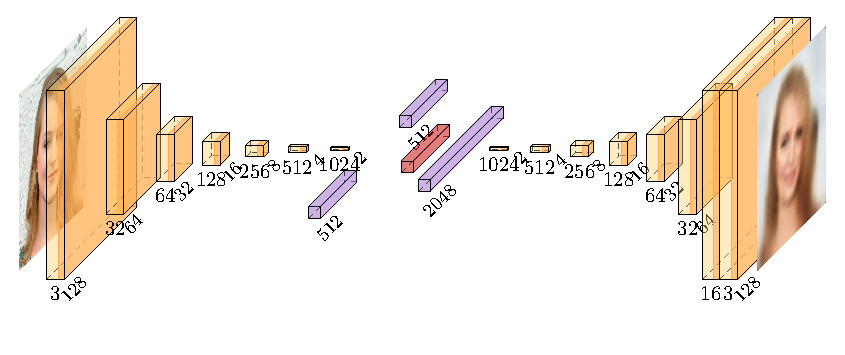
\includegraphics[width=\textwidth]{figs/vae.pdf}
    \caption{Encoder-Decoder Architecture used for this work}\label{fig:vae}
\end{figure*}
We learn a $512$-dimensional representation of the $128\times 128$ images and encode all the \texttt{CACD2000} images.
Once all the images have been encoded in $\mathbb{R}^{512}$ it is possible to use the local linear estimator of the gradient studied in this work to derive the gradient of the age with respect to the latent variable, making it possible to produce a new version of the input image that appears either older or younger as done in Figure~\ref{fig:age}. By computing a local estimate of the gradient, we are able to derive a more meaningful change when the age is not perfectly disentangled.
\begin{figure}[H]
    \centering
    \begin{tikzpicture}
        \node[inner sep=0pt] (encoded) at (0,0)
            {
\includegraphics[width=.1\textwidth]{figs/encoded.jpg}};
        \node[inner sep=0pt] (aged) at (6,0)
            {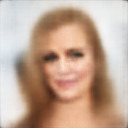
\includegraphics[width=.1\textwidth]{figs/aged.jpg}};
        \draw[->,thick] (encoded.east) -- (aged.west)
            node[midway,fill=white] {$z + 0.1 \times \nabla m(z)$};
    \end{tikzpicture}
    \caption{Extracting the direction of interest for aging.}\label{fig:age}
\end{figure}
Note that the quality of the image reconstruction and generation is here solely limited by the choice of the encoding and decoding model and is not related to the methods introduced in this paper, significant advances in the quality of the decoding have been made in the recent years and if a better quality and less blurry decoded output is desired we encourage the reader to replace the decoder with a \texttt{PixelCNN} architecture such as presented in~\cite{salimansPixelCNNImprovingPixelCNN2017}. The quality of the gradient is also significantly impacted by the quality of the annotations as \texttt{CACD200} is an automatically annotated and noisy dataset. 

Using our estimator it is possible to estimate the gradient $\nabla m$ of $\mathbb{E} [ Y \mid Z = z ]$ with respect to the latent variable $Z$ (illustrated in the Appendix). It is then possible to analyse the sparsity of $\nabla m$ to quantify the quality of the disentanglement for varying level of $\beta$ by quantifying how far from a single dimension the gradient for the age is concentrated. As the true dimension is unknown, we instead measure the angular distance to all dimensions reweighted by the magnitudes of the partial derivatives:
\begin{equation}
    \begin{split}
        &\sum_i \frac{\lvert\hat \nabla_i m(x) \rvert}{\lvert \hat \nabla m(x) \rvert} \cos (e_i, \frac{1}{n} \sum_k \lvert \hat \nabla m(x) \rvert), \\
        \text{where} \quad &\cos (a, b) = \frac{a \cdot b}{\lVert a \rVert \lVert b \rVert}.
    \end{split}
\end{equation}
We observe in Figure~\ref{fig:disentangle} that as $\beta$ increases the age slowly become disentangled, as expected if one considers the age to be an important and independent characteristic of human faces.
\begin{figure}[H]
    \centering
    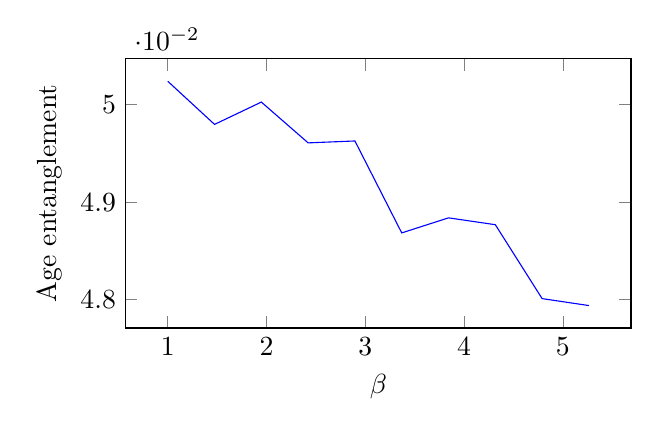
\begin{tikzpicture}
\begin{axis}[xlabel={$\beta$}, ylabel={Age entanglement},width=8cm,height=5cm]
    \addplot+[no marks]
        table[row sep={\\}]
        {
            x  y  \\
            1.0  0.05024031549692154  \\
            1.4736842  0.04979776591062546  \\
            1.9473684  0.05002676323056221  \\
            2.4210527  0.04960823431611061  \\
            2.8947368  0.049627795815467834  \\
            3.368421  0.04868478327989578  \\
            3.8421052  0.04883917048573494  \\
            4.3157897  0.048768892884254456  \\
            4.7894735  0.0480106882750988  \\
            5.263158  0.04793939366936684  \\
        }
        ;
\end{axis}
\end{tikzpicture}

    \caption{Quality of disentanglement with respect to the age} \label{fig:disentangle}
\end{figure}

While not an entirely adequate metric for disentanglement, not only because disentanglement does not necessarily require the dimensions to be the one an observer expected but more importantly because this metric requires an annotated dataset; we believe this metric can be useful for practitioners. By measuring how close the estimated gradients are to the axis, with respect to an annotated dataset of characteristics of interest, a practitioner can ensure his model is sufficiently disentangled for downstream tasks such as face manipulation by a user. We also believe it is possible to design an end-to-end differentiable framework in order to force disentanglement to consider the characteristics of interest: our estimator is the solution to a convex optimization program and as such admits an adjoint; it is therefore possible to fit a local linear estimator inside an automatic differentiation framework such as done in~\cite{agrawalDifferentiableConvexOptimization2019}.
